% !TeX spellcheck = cs_CZ
%{\tikzset{external/prefix={tikz/MAI/}}
% \tikzset{external/figure name/.add={ch10_}{}}
%---------------------------------------------------------------------------------------------------
% file ppst.tex
%---------------------------------------------------------------------------------------------------
\chapter{Počet Pravděpodobnosti}\label{mai:IchapIII}
\minitoc
  Slovo pravděpodobnost používáme velmi často. Jaký však je jeho přesný význam? Jsme přesvědčeni, 
  že pravděpodobnost výhry ve sportce je velmi malá. Ani pravděpodobnost, že se vyplní předpověď 
  počasí, nepovažujeme mnohdy za výraznou. Přesto je mezi oběma příklady obrovský kvantitativní 
  rozdíl. Zkusme význam pojmu pravděpodobnost ukázat pomocí konkrétních číselných příkladů.
  
  \begin{itemize}
    \item \textbf{Příklad se střelcem}: Sportovní střelec střílí na terč série \num{100} ran. 
          Předpokládejme, že podmínky při střelbě jsou stále stejné. Stejná je zbraň, terč, 
          vzdálenost, povětrnostní podmínky i momentální zdravotní stav střelce. Při hodnocení 
          střelcova „mistrovství“ někdo řekne, že střelec zasáhne terč s pravděpodobností 
          \num{92}\%. Jak tomu rozumět? Znamená to, že v souboru sérií výstřelů jsou velmi časté 
          ty, v nichž zasáhl střelec terč \num{92}-krát. Samozřejmě, není řídké, že se objeví i 
          série s \num{93} nebo \num{94} zásahy, ale také s \num{91} nebo \num{90}. Vyloučen není 
          ani případ s úspěšností \num{96} či \num{88}, a dokonce i stovku bychom mohli zaznamenat. 
          Situace výrazně odlišné od \num{92} zásahů však budou řídké, a to tím více, čím více se 
          úspěšnost série liší od \num{92} oběma směry.
    \item \textbf{Příklad se zmetky}: Koupíte si výrobek u firmy, o které je známo, že vyrábí 
          zmetky s pravděpodobností 0,16\%? Situaci lze posuzovat obdobně jako úspěšnost střelce. 
          Budeme-li například zkoumat série obsahující 1000 výrobků, bude každá z nich obsahovat „v 
          průměru“ 16\% zmetků. Z příkladu se střelcem již zhruba víme, jak posuzovat slovo v 
          průměru.
  \end{itemize}
  
  V této kapitole se budeme pravděpodobnostmi zabývat podrobněji. Zjistíme, že i když se týkají 
  náhodných jevů, platí i pro ně jisté zákonitosti.
    
  \section{Pravděpodobnost}\label{mai:IchapIIIsecI}
    V úvodních příkladech jsme si vyložili, jak intuitivně chápat pojem pravděpodobnost. Jednalo se 
    v nich o posouzení průměrné úspěšnosti ve velkém souboru operací či úkonů prováděných za 
    stejných podmínek, šlo tedy o jakousi „průměrnou“ pravděpodobnost. Nyní definujeme 
    pravděpodobnost matematicky.
    
    \subsection{Co se pravdě podobá - definice pravděpodobnosti}
      Pro definici pravděpodobnosti použijeme pojmu \emph{náhodný pokus}, jehož význam si ukážeme 
      na příkladu. Dobrým příkladem náhodných pokusů je třeba házení mincí, hraní kostkou, výběr 
      karet z balíčku, vidíme-li pouze jejich rub, apod. Budeme třeba házet kostkou. Abychom si 
      situaci zbytečně nekomplikovali, budeme předpokládat, že všechny výsledky hodu kostkou 
      (náhodné pokusy) jsou stejně časté, žádný z nich není nijak preferován\footnote{Kostka by 
      tedy měla být homogenní, plocha, na kterou po hodu dopadne, vodorovná, kvalita povrchu všech 
      stěn kostky stejná (žádná stěna by třeba neměla být natřena lepidlem), apod.}. Počet možných 
      výsledků jednotlivého hodu je \(N = 6\) (kostka má \num{6} stěn, na každé je vyznačen odlišný 
      počet ok, tedy \num{1} až \num{6}). Jednotlivé situace, které mohou nastat, nazýváme 
      náhodnými jevy. Náhodným jevem \(A\) tak může být situace \emph{„padne číslo \num{2}“}, jiným 
      náhodným jevem \(B\) situace \emph{„padne číslo dělitelné třemi“}, apod. Počet situací, kdy 
      výsledek hodu lze hodnotit tak, že určitý jev nastal, označíme \(M\). Například pro jev \(A\) 
      \emph{„padne číslo \num{2}“} je \(M(A)= 1\), pro jev \(B\) \emph{„padne číslo dělitelné 
      třemi“} je \(M(B) = 2\) (počet ok \num{3} nebo \num{6}). Můžeme také definovat jev \(O\) 
      \emph{„nepadne žádné číslo“} (\(M(0) = 0\)) nebo jev \(J\) \emph{„padne jakékoli číslo“} 
      (\(M(J) = 6\)).
      
      \begin{definition}
        Pravděpodobností jevu rozumíme podíl
        \begin{equation}\label{mai:eq011}
          p = \frac{M}{N} = \frac{\text{počet případů příznivých}}{\text{počet případů možných}}.
        \end{equation}  
        Počtem případů možných jsme zkráceně nazvali počet všech možných výsledků náhodného 
        pokusu, počtem případů příznivých pak počet všech takových výsledků pokusu, při nichž daný 
        jev nastal.
      \end{definition}
      Je zřejmé, že hodnota pravděpodobnosti jakéhokoli jevu je nezáporná a může nabývat hodnoty 
      nejvýše \num{1}, tj. \(0 <p< 1\). Jev s \emph{nulovou pravděpodobností} se nazývá 
      \textbf{nemožný}, jev s \emph{jednotkovou pravděpodobností} je \textbf{jistý}. V našem 
      příkladu s kostkou tak dostáváme
      \begin{equation*}
        p(A) = \frac{1}{6}, \qquad p(B) = \frac{2}{6} = \frac{1}{3}, \qquad
        p(O) = 0, \qquad p(J) = 1.
      \end{equation*}  

      %--Barevné ponožky----------------------------------------------
      % !TeX spellcheck = cs_CZ
\begin{example}
 \label{mai:exam006}
  \textbf{Barevné ponožky}:\newline\small
  V zásuvce jsou ponožky tří barev. Červené (\textbf{Č}), zelené (\textbf{Z}) a modré (\textbf{M}). 
  Je jich tam od každé barvy hodně. Student jde na schůzku a chce si vzít čisté ponožky. Náhle 
  zhasne světlo. Student vytáhne potmě dvě ponožky. Jaká je pravděpodobnost, že ponožky budou mít 
  stejnou barvu? Vyjmenujme případy, které mohou při vytažení dvou ponožek nastat: (\textbf{Č+Č}), 
  (\textbf{Č+Z}), (\textbf{Z+Č}), (\textbf{Č+M}), (\textbf{M+Č}), (\textbf{Z+Z}), (\textbf{Z+M}), 
  (\textbf{M+Z}), (\textbf{M+M}). Je tedy \(n = 9\). Příznivé situace jsou tří, (\textbf{Č+Č}), 
  (\textbf{Z+Z}), (\textbf{M+M}). Pravděpodobnost je tedy 1/3. (Převzato z 
  \cite[s.~200]{Musilova2009MA1}) 
\normalsize
\end{example}
      %---------------------------------------------------------------
    \subsection{Cifry, kostky, karty - kombinatorické opakování}
      Příklad s ponožkami byl velmi jednoduchý. Podařilo se nám vyjmenovat všechny případy možné i 
      všechny případy příznivé, neboť obojího bylo docela málo. Daleko běžnější jsou však situace, 
      kdy výčet případů není schůdný. A tehdy potřebujeme \textbf{kombinatoriku}.
      
      Nechť \(\mathcal{M}\) je \(n\)-prvková množina, z níž budeme provádět výběry \(k\) prvků 
      podle určitých pravidel. Prvky množiny \(\mathcal{M}\) nemusíme nijak konkretizovat. Abychom 
      si však o výběrech a pravidlech pro jejich tvorbu dokázali udělat nějakou názornou představu, 
      je taková konkretizace vhodná. Prvky množiny \(\mathcal{M}\): mohou být třeba žáci ve třídě, 
      barvy, hrací karty, apod. Výběry mohou představovat třeba družstva pro odbíjenou, signály 
      tvořené barevnými praporky, možnosti rozdání karet při mariáši, apod. Jednotlivé typy výběrů 
      získaly své názvy právě na základě pravidel stanovených pro jejich vytváření. Rozhodující 
      jsou dvě základní kritéria:
      \begin{itemize}\addtolength{\itemsep}{-0.5\baselineskip}
        \item Je pro tvorbu výběru podstatné pořadí prvků ve výběru či nikoliv?
        \item Mohou se prvky ve výběru opakovat či nikoliv?
      \end{itemize}
      
      Typy výběrů shrnuje následující diagram:
      \begin{figure}[ht!] %\ref{mai:fig021}
        \centering
        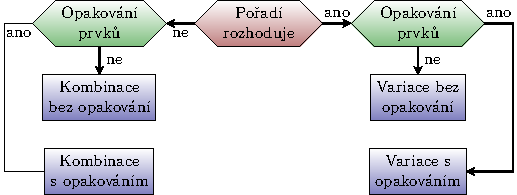
\includegraphics[width=0.7\linewidth]{mai_fig021.pdf}
        \caption{Typy výběrů. \cite[s.~201]{Musilova2009MA1}}
        \label{mai:fig021}
      \end{figure}

      Představuje-li daný výběr například volejbalové družstvo osmi děvčat (šest hráček a dvě 
      náhradnice), které bude reprezentovat v soutěži třídu osmou bé, do níž chodí \num{25} děvčat 
      a \num{18} chlapců, jedná se o výběr \(k - 8\) prvků z počtu \(n = 25\) prvků. Chlapce nelze 
      postavit do družstva volejbalistek. Každý výběr možného družstva bude představovat 
      \emph{kombinaci bez opakování}, neboť pořadí hráček nehraje roli a třeba Aničku Novákovou 
      máme ve třídě jen jednu. Budeme-li však chtít vytvářet z deseti cifer \(0, 1, \ldots, 9\) 
      trojciferná čísla, pak tyto výběry tří prvků z deseti (\(k = 3\), \(n = 10\)) jsou 
      \emph{variacemi s opakováním}. Čísla \num{125}, \num{512}, \num{251}, \num{215}, \num{521} a 
      \num{152} jsou totiž různá, a například \num{222} je také trojciferné číslo. Kombinace s 
      opakováním bychom mohli vytvářet třeba i při výběru různobarevných ponožek ze zásuvky a 
      konečně \emph{variacemi bez opakování} by mohly být dejme tomu trojbarevné signály (\(k = 
      3\)) tvořené trojicemi barevných hadříků vybíraných z \(n\) barev (pro \(n = 3\) třeba zrovna 
      z těch ponožek). Nyní bychom však rádi věděli, jak pro zadané hodnoty \(n\) a \(k\) určit 
      počet všech možných výběrů předepsaného typu. Ukážeme si to na příkladech.

      %--Šance milion-------------------------------------------------
      % !TeX spellcheck = cs_CZ
\begin{mdframed}[style=mdexam]
  \begin{example}\label{mai:exam007}
    \textbf{Šance milion}:\newline
    „Znáte nějakou jinou hru, kde můžete denně vyhrát milion?“ Tento nebo jiný, obdobně nepříliš
    vtipný reklamní slogan propaguje v televizi hru, jejímž cílem je uhodnout šestici tažených cifer
    ve správném pořadí. (Hru raději nehrajte, pravděpodobnost výhry je mizivá.) Tah se provádí
    následovně: V každém ze šesti bubnů, očíslovaných pořadovými čísly \num{1} až \num{6}, je
    připraveno deset míčků opatřených ciframi \(0, 1, \ldots, 9\). Z prvního bubnu se náhodně
    vylosuje jedna cifra (deset možností). Poté se náhodně vylosuje jedna cifra z druhého bubnu
    (opět deset možností). Možností vzniku uspořádané dvojice cifer (jedna cifra z prvního a druhá z
    druhého bubnu) je již sto (každou možnost výsledku u prvního bubnu lze kombinovat s každou
    možností výsledku z druhého bubnu). Losování pokračuje u třetího, čtvrtého, pátého a šestého
    bubnu. Celkový počet možností je \num{1e6}, tedy \textbf{milion}. (Šance získat výhru, tedy
    vyhrát milion, je ovšem pouze jedna milióntina, neboť z milionu možností je pouze jedna skutečně
    tažena.) 
  \end{example}
\end{mdframed}
      %---------------------------------------------------------------
      
      Zobecněním předchozího příkladu získáváme vzorec pro počet \textbf{variací s opakováním} 
      \emph{k}-té třídy z \(n\) prvků. Při tahu totiž záleží na pořadí bubnů a každý buben obsahuje 
      všechny cifry. Výsledky tahů z jednotlivých bubnů se tedy mohou opakovat. Pokud by bubnů bylo 
      \(k\) a v každém \(n\) různých cifer, dostali bychom pro \textbf{variace s opakováním 
      \(k\)-té třídy z \(n\) prvků} celkový počet
      \begin{equation}\label{mai:eq007}
        \boxed{V_k' = n^k}\, .
      \end{equation}

      %--Modifikovaná šance milion------------------------------------
      % !TeX spellcheck = cs_CZ
\begin{example}\label{mai:exam008}
  \textbf{Modifikovaná šance milion}:\newline
  Představme si hru z předchozího příkladu upravenou takto: K dispozici bude jen jeden buben s 
  ciframi \(0, 1, \ldots, 9\), každá cifra je v bubnu obsažena pouze jednou. Opět máme losovat 
  uspořádanou \textbf{šestici cifer}. Nyní se však jedná o \textbf{variace šesté třídy z deseti 
  prvků bez opakování}. S jediným bubnem musíme totiž provést šest losování, přičemž při každém 
  losování ubude z bubnu jedna cifra. Při prvním tahu je deset možností, při druhém již jen devět, 
  atd., při šestém již pouze pět možností. Celkem je tedy \(10 \cdot 9 \cdots 5 = \num{151200}\) 
  možností.
\end{example}
      %---------------------------------------------------------------
      
      Uvážíme-li, že v předchozím příkladu je \(n = 10\) a \(k = 6\), dostáváme pro \textbf{počet 
      variací bez opakování \(k\)-té třídy z \(n\) prvků} obecný vztah
      \begin{align}
        V_k(n) &= n(n-1)(n-2)\cdots(n-k+1)  \nonumber \\
        \shortintertext{neboli}
        V_k(n) &= \frac{n!}{(n-k)!}\, .    \label{mai:eq008}
      \end{align}
      Poznamenejme, že \(n!\) značí \textbf{faktoriál}, \(n! = n(n - 1)\cdots 3 \cdot 2 \cdot 1\). 
      Pro nulu definujeme \(0! = 1\). Je zřejmé, že při vytváření variací bez opakování musí být 
      \(k\leqq n\). Variace bez opakování \(n\)-té třídy z \(n\) prvků se nazývají 
      \textbf{permutace}. Každá z nich představuje určité uspořádání těchto \(n\) prvků. Platí
      \begin{equation}\label{mai:eq009}
        \boxed{P(n) = V_n(n) = n!}\, .
      \end{equation}
      
      Nyní odvodíme vzorec pro počet \textbf{kombinací \(k\)-té třídy z \(n\) prvků bez opakování}. 
      Již jsme si řekli, že \emph{kombinací} rozumíme takový výběr z celkového počtu \(n\) prvků, 
      který obsahuje určitých \(k\) prvků nezávisle na jejich pořadí. Představme si, že máme k 
      dispozici všechny variace bez opakování \(k\)-té třídy ze zmíněných \(n\) prvků. Vezměme 
      kteroukoli z nich. Soubor všech variací \(k\)-té třídy z \(n\) prvků však obsahuje i další 
      variace, lišící se od té naší jen pořadím prvků. Celkem je takových variací (i s tou první) 
      \(k!\) a z hlediska kombinací představují totéž. Soubor variací se tak rozpadá na podsoubory, 
      z nichž každý obsahuje \(k!\) variací lišících se navzájem pouze pořadím prvků. Každý z 
      těchto podsouborů představuje však jedinou kombinaci. Počet kombinací \(k\)-té třídy z \(n\) 
      prvků bez opakování je tedy
      \begin{equation}\label{mai:eq010}
        \boxed{C(k) = \frac{V_k(n)}{P(k)} = \frac{n!}{(n-k)!\,k!} = 
               \begin{pmatrix}
                n \\
                k
               \end{pmatrix}}\, .
      \end{equation}
      
      Pro odvození vzorce pro \textbf{kombinace s opakováním} použijeme opět příkladu.
      %--Kuličky v přihrádkách----------------------------------------
      % !TeX spellcheck = cs_CZ
\begin{mathexam}{Kuličky v přihrádkách}{exam009}
  Máme kuličky \(n\) různých barev, v každé barvě máme tolik kuliček, kolik bude potřeba. Naším
  úkolem je vytvářet výběry \(k\) kuliček. Na \textbf{pořadí barev nezáleží}, kuliček jedné barvy
  může být ve výběru libovolný počet \(0\leqq s \leqq k\). Výběry budeme vytvářet tak, že budeme
  kuličky dávat do \(n\) přihrádek, z nichž každá bude vyhrazena pro určitou barvu. Pokud tedy v
  daném výběru zrovna nebude třeba modrá kulička, bude přihrádka vyhrazená pro modrou barvu prázdná.
  Budou-li v daném výběru právě tři červené kuličky, budou umístěny v přihrádce vyhrazené pro
  červenou barvu. Vidíme, že pokud konkrétním přihrádkám přisoudíme konkrétní barvy, samotné kuličky
  by již barevné být nemusely, stačily by třeba kuličky skleněné, bezbarvé. Zůstane-li například
  přihrádka pro modrou barvu prázdná, víme, že daný výběr neobsahuje modrou barvu. Budou-li v
  přihrádce pro červenou barvu tři (bezbarvé) kuličky, víme, že daný výběr obsahuje červenou barvu
  třikrát. Příklad takové situace ukazuje následující schéma:
  
  {\centering
    \luafigure[0.9]{mai_fig033.pdf}
    \par}

  Náš úkol můžeme přeformulovat takto: Je třeba rozmístit \(k\) kuliček do \(n\) přihrádek. V každé
  přihrádce může být obecně \(s\) kuliček, kde \(0\leqq s \leqq k\), přitom celkový počet kuliček
  musí být samozřejmě stále \(k\). Můžeme si představit, že \(k\) kuliček máme položených v řadě na
  polici mezi dvěma pevnými stěnami (krajní svislé čáry v předchozím schématu) a různé způsoby
  rozmístění kuliček do přihrádek provádíme přemísťováním pohyblivých přepážek. Kdybychom například
  v předchozím schématu přesunuli druhou svislou čáru, počítáno zleva, až za první kuličku v
  přihrádce na červenou barvu, dostaneme uspořádání, při němž je v přihrádce na modrou barvu jedna
  kulička a v přihrádce na červenou barvu dvě kuličky. Tedy takto:

  {\centering
    \luafigure[0.9]{mai_fig034.pdf}
  \par}

  Mezi dvěma krajními pevnými stěnami máme tedy k dispozici \(k\) pozic pro kuličky a \((n - 1)\)
  pozic pro pohyblivé přepážky. Celkem tedy \((n + k - 1)\) pozic, na které můžeme libovolně
  rozmísťovat \(k\) kuliček a \((n - 1)\) přepážek. Do těchto \((n + k - 1)\) pozic můžeme umístit
  \(k\) kuliček \(C_k'(n)\) způsoby, kde
  \begin{equation}\label{MAI:eq011}
    \boxed{C_k'(n) =  \binom{n + k - 1}{k} = \binom{n + k - 1}{n -1}}\, .
  \end{equation}
  Na zbylé pozice již musíme umístit přepážky. Nebo naopak, nejprve umístíme \((n - 1)\) přepážek a
  potom kuličky. Výsledek je stejný, jak je vidět z předchozího vzorce. Protože jsme vytváření
  kombinací s opakováním \(k\)-té třídy z \(n\) prvků převedli na úlohu o rozmísťování kuliček do
  přihrádek, udává získaný vzorec právě počet takových kombinací. Aby měl vzorec smysl, musí platit
  \(n + k - 1 \geqq k\), tedy \(n \geqq 1\).

  Komu nevyhovuje představa kuliček v přihrádkách a má raději čísla, může uvažovat následovně: Tak
  jako je každé číslo v desítkové soustavě zapsáno pomocí cifer \(0, 1, 2, \ldots , 8, 9\), je k
  jeho zápisu ve dvojkové soustavě potřeba pouze dvou cifer, nuly a jedničky. Představme si nyní
  přepážku jako jedničku a kuličku jako nulu. Náš úkol zjistit počet všech možných způsobů rozdělení
  \(k\) kuliček do \(n\) přihrádek, ohraničených \((n+1)\) přepážkami, můžeme převést na
  ekvivalentní problém: Kolik dokážeme najít čísel, která jsou ve dvojkové soustavě zapsána právě
  \(k\) nulami a \((n + 1)\) jedničkami, požadujeme-li, aby první i poslední cifrou byla jednička?
  Odpověď je jednoduchá. Máme k dispozici \((n+k+1)\) pozic pro cifry. První a poslední pozice jsou
  pevně obsazeny jedničkami, volných pozic je tedy pouze \((n + k - 1)\). Počet všech různých
  způsobů, kterými na \(k\) z těchto pozic můžeme umístit nuly, je roven počtu kombinací \(k\)-té
  třídy z \((n + k - 1)\) prvků. Na zbylé pozice již musíme umístit jedničky. Komplementárně,
  budeme-li hledat počet všech možných způsobů, jak na \((n-1)\) pozic umístit jedničky, dostaneme
  shodný výsledek, v souhlasu se vzorcem (\ref{mai:eq010}).
\end{mathexam}
      %---------------------------------------------------------------
      
      %--Obsazování kvantových stavů----------------------------------
      % !TeX spellcheck = cs_CZ
\begin{example}\label{mai:exam010}
  \textbf{Obsazování kvantových stavů}:\newline\small
  Úloha o kuličkách a přihrádkách má přímou aplikaci v \textbf{kvantové fyzice}. Představme si, že 
  fyzikální soustava je tvořena \(k\) částicemi. Každá částice se nachází v určitém stavu, v němž 
  jí můžeme přisoudit fyzikální charakteristiky, které jsou s tímto stavem spojeny (třeba energii, 
  moment hybnosti, apod.). Jednotlivé stavy jsou pak rozlišitelné právě pomocí těchto 
  charakteristik. Dejme tomu, že přípustných stavů je \(n \geqq 1\). Problémem kvantové fyziky je 
  to, že kvantové částice jsou nerozlišitelné. Nepoznáme jednu od druhé. Je to stejné, jako bychom 
  měli \(k\) naprosto stejně vypadajících kuliček, které nemáme nijak očíslovány. Záměna dvou 
  částic (nerozlišitelných kuliček) se nepozná, nevede tedy ke změně stavu fyzikální soustavy. Pro 
  hodnoty fyzikálních charakteristik soustavy jako celku je tedy důležité jen to, kolik částic je v 
  každém z přípustných stavů. Musíme se tedy zajímat o to, kolika způsoby lze našich \(k\) 
  \textbf{nerozlišitelných částic} (kuliček) umístit do \(n\) \textbf{stavů} (přihrádek). Kvantové 
  částice jsou však dvojího druhu, \textbf{fermiony} (například elektrony, neutrony, protony, jádra 
  s lichým počtem nukleonů) a \textbf{bosony} (například fotony, mezony, jádra se sudým počtem 
  nukleonů). Rozdíl mezi nimi je ten, že bosony se „dobře snášejí“, a proto jich může být v jednom 
  stavu i více. 
  \begin{itemize}\addtolength{\itemsep}{-0.5\baselineskip}
    \item Počet možností, jak rozmístit \(k\) \textbf{bosonů} po \(n\) stavech je tedy
          \begin{equation*}
            N_{\text{boson}} = 
              \begin{pmatrix}
                n + k - 1 \\
                    k
               \end{pmatrix}
          \end{equation*}
    \item S \textbf{fermiony} je tomu jinak. \textbf{Pauliho vylučovací princip} jim zakazuje, 
          aby v daném stavu byl více než jeden fermion. Stav může být buď prázdný, nebo obsazen 
          jedním fermionem. V takovém případě musí být \(n \geqq k\) a v každé přihrádce může být 
          nejvýše jedna kulička. Situace tak odpovídá \textbf{kombinacím bez opakování \(k\)-té 
          třídy z \(n\) prvků}, tj.
          \begin{equation*}
            N_{\text{fermion}} = 
              \begin{pmatrix}
                n  \\
                k
              \end{pmatrix}
          \end{equation*}
  \end{itemize}
\normalsize
\end{example}
      %---------------------------------------------------------------
      
      Získané kombinatorické vzorce nyní použijeme při řešení základních úloh o pravděpodobnostech. 
      V každé úloze bude důležité
      \begin{itemize}
        \item definovat jev \(A\), jehož pravděpodobnost počítáme,
        \item určit počet \(N\) případů možných, tj. počet všech možných výsledků pokusu, při 
              kterém sledujeme, zda jev \(A\) nastal či nenastal,
        \item určit počet \(M\) případů příznivých, tj. počet těch výsledků daného pokusu, při 
              kterých jev \(A\) nastal.
      \end{itemize}

      %--Výhra ve sportce---	----------------------------------------
      % !TeX spellcheck = cs_CZ
\wikitextrule
\begin{example}\label{mai:exam052}
  \textbf{Výhra ve sportce}\newline\small
  Jaká je pravděpodobnost hlavní výhry ve sportce? Všichni víme, že malá, ale máme představu, jak 
  malé toto číslo je? Při sportce se losuje \(k = 6\) čísel a jedno dodatkové z celkového počtu \(n 
  = 49\) čísel. (Dříve byla čísla spojena s názvy sportů, odtud název „sportka“ .) Na pořadí čísel 
  ve výběru nezáleží, vytažené číslo se do hry nevrací. Jde tedy o \textbf{kombinace bez 
  opakování}. Hlavní výhra požaduje uhodnout všech \num{6} tažených čísel. Jev \(A\) je tedy 
  definován takto:
  
  \begin{itemize}
    \item Jev \(A\): Bude taženo právě oněch \num{6} čísel, která jsem vsadil.
          Počet možností, které při tahu sportky mohou nastat (počet případů možných), je \(N = 
          \begin{pmatrix} n \\ k\end{pmatrix} =  \begin{pmatrix} 49 \\ 6 \end{pmatrix} \). Hlavní 
          výhru představuje jediná kombinace, počet příznivých případů je proto \(M = 1\). 
          Pravděpodobnost hlavní výhry ve sportce, tj. pravděpodobnost jevu \(A\), je
          \begin{equation*}
            p(A) = \dfrac{M}{N} = \dfrac{1}{\begin{pmatrix} 49 \\ 6 \end{pmatrix}} 
                 = \dfrac{43!6!}{49!} = \dfrac{720}{49\cdot48\cdot47\cdot46\cdot45\cdot44} \simeq 
                 \num{7e-8}
                 = \SI{7e-6}{\percent}
          \end{equation*}
          Pravděpodobnost hlavní výhry je velmi malá, sedm milióntin procenta. 
    \item A o kolik lepší to bude s pravděpodobností některé z vedlejších výher? Tak třeba pátá 
          cena znamená, že je nutné ze šesti tažených čísel uhodnout libovolné tři. Jev \(A\) je 
          tedy: Ze šesti čísel, která jsme vsadili, budou v tažené kombinaci obsažena právě tři 
          libovolná z nich. Počet \(N\) zůstává stejný jako v předchozí části úlohy. Je třeba jen 
          určit \(M\). Každý příznivý případ vzniká tak, že trojice správných čísel (výběry tří ze 
          šesti) je doplněna trojicí chybných čísel (výběry tří ze čtyřiceti tří). Tedy \(M = 
          \begin{pmatrix}6 \\ 3\end{pmatrix}\begin{pmatrix} 49 - 6 \\ 3\end{pmatrix} =  
          \begin{pmatrix} 6 \\ 3\end{pmatrix}\begin{pmatrix} 43 \\ 3 \end{pmatrix}\),
          \begin{align*}
            p(A) &= \dfrac{M}{N} 
                  = \dfrac{\begin{pmatrix} 6 \\ 3\end{pmatrix}
                           \begin{pmatrix} 43 \\ 3 \end{pmatrix}}
                          {\begin{pmatrix} 49 \\ 6\end{pmatrix} }                
                  =\left(\dfrac{6!}{3!\cdot3!}\right)\left(\dfrac{43!}{40!\cdot3!}\right)
                   \left(\dfrac{43!6!}{49!}\right)                                            \\
                 &=\dfrac{120\cdot43\cdot42\cdot41\cdot720}
                         {49\cdot48\cdot47\cdot46\cdot45\cdot44\cdot36} 
                  \simeq\num{0.018}.
          \end{align*}
          Tato pravděpodobnost již zanedbatelná není, na rozdíl od finanční částky, jíž bývá 
          ohodnocena pátá cena. Sázení sportky může domácímu rozpočtu spíše ublížit.
    \item Třetí, resp. čtvrtá cena jsou, podobně jako první a pátá, definovány velmi jednoduše. Je 
          třeba uhodnout pět, resp. čtyři ze šesti tažených čísel. V případě druhé ceny hraje roli
          dodatkové číslo. Druhou cenu získává ten, kdo uhodl pět ze šesti čísel vylosovaných v 
          prvním tahu a ještě navíc číslo dodatkové, které se losuje ze zbylých \num{43} čísel, jež 
          zůstala po prvním tahu v osudí. Jev \(A\) je tedy definován takto:
          
          Ze šesti čísel, která jsem vsadil, bude při prvním tahu vylosováno libovolných pět a v 
          druhém tahu bude vylosováno právě to dodatkové číslo, které jsem vsadil. Počet případů 
          příznivých je pouze \(M = \begin{pmatrix}6 \\ 5\end{pmatrix}\), neboť šestým číslem 
          nemůže být libovolné ze \num{43} čísel, která nebyla v prvním tahu vylosována, ale 
          musí to být právě číslo dodatkové. Pravděpodobnost jevu \(A\) je
          \begin{equation*}
            p(A)  = \dfrac{M}{N} 
                  = \dfrac{\begin{pmatrix} 6  \\ 5\end{pmatrix}}
                          {\begin{pmatrix} 49 \\ 6\end{pmatrix}}
                  \simeq\num{4.2e-17}.
          \end{equation*}
          
          Pokud bychom jako jev \(A\) označili výhru jakékoliv ceny, dostaneme
          \begin{align*}
            M &= \sum_{6}^{k=3}\begin{pmatrix} 6  \\   k  \end{pmatrix}
                               \begin{pmatrix} 43 \\ 6 - k\end{pmatrix}  +
                               \begin{pmatrix} 6  \\   5  \end{pmatrix}                      \\
              &= \begin{pmatrix} 6 \\ 3\end{pmatrix}\begin{pmatrix} 43 \\ 3\end{pmatrix} +
                 \begin{pmatrix} 6 \\ 4\end{pmatrix}\begin{pmatrix} 43 \\ 2\end{pmatrix} +
                 \begin{pmatrix} 6 \\ 5\end{pmatrix}\begin{pmatrix} 43 \\ 1\end{pmatrix} +
                 \begin{pmatrix} 6 \\ 6\end{pmatrix}\begin{pmatrix} 43 \\ 0\end{pmatrix} +
                 \begin{pmatrix} 6 \\ 5\end{pmatrix},                                        \\
           p(A) &= \dfrac{\begin{pmatrix}  6 \\ 3\end{pmatrix}
                          \begin{pmatrix} 43 \\ 3\end{pmatrix}  +
                          \begin{pmatrix}  6 \\ 4\end{pmatrix}
                          \begin{pmatrix} 43 \\ 2\end{pmatrix}  +
                          \begin{pmatrix}  6 \\ 5\end{pmatrix}
                          \begin{pmatrix} 43 \\ 1\end{pmatrix}  +
                          \begin{pmatrix}  6 \\ 6\end{pmatrix}
                          \begin{pmatrix} 43 \\ 0\end{pmatrix}  +
                          \begin{pmatrix}  6 \\ 5\end{pmatrix}}
                         {\begin{pmatrix} 49 \\ 6\end{pmatrix}} =\simeq\num{0.019}.
          \end{align*}
          Všimněte si, že tento výsledek je roven součtu pravděpodobností výhry páté, čtvrté, 
          třetí, druhé a hlavní ceny. Později si tento závěr ještě připomeneme.
  \end{itemize}  
  \normalsize
\end{example}
      %---------------------------------------------------------------

      %--Losování karet-----------------------------------------------
      % !TeX spellcheck = cs_CZ
\wikitextrule
\begin{example}\label{mai:exam053}
  \textbf{Losování karet}\newline\small
    Máme karetní hru mariáš, která obsahuje celkem \num{32} karet osmi hodnot \num{7}, \num{8}, 
    \num{9}, \num{10}, J (kluk), Q (dáma), K (král), A (eso), každá hodnota je ve čtyřech barvách, 
    červené barvy jsou \(\heartsuit\) (srdce) a \(\lozenge\) (kára), černé barvy jsou \(\spadesuit\)
    (piky) a \(\clubsuit\) (kříže). Jaká je pravděpodobnost, že při náhodném vylosování deseti 
    karet budou 
    mezi nimi:
    \begin{enumerate}[label=\Alph*]
      \item právě dvě esa,
      \item alespoň dvě esa,
      \item nejvýše dvě esa,
      \item alespoň šest karet stejné barvy,
      \item právě dvě dámy a alespoň jeden kluk,
      \item právě dvě dámy nebo alespoň jeden kluk?
    \end{enumerate}

    Písmena (A) až (F) představují různé části úlohy a také zároveň definují jevy, jejichž 
    pravděpodobnost počítáme. Jedná se opět o kombinace. Nezáleží totiž na pořadí, v jakém karty 
    vytahujeme. Důležité je jen to, zda jsou vyjmenované karty ve výběru obsaženy. Počet možných 
    výsledků náhodného vylosování deseti karet z dvaatřiceti, tj. počet případů možných, je pro 
    všechny části úlohy stejný,
    \begin{equation*}
      N = \begin{pmatrix} 32 \\ 10\end{pmatrix} 
        = \dfrac{32\cdot31\cdots24\cdot23}{10\cdot9\cdots2\cdot1} = \num{64512240}.
    \end{equation*}
    
    Počítejme nyní případy příznivé pro jednotlivé jevy \(A\) až \(F\) a pravděpodobnosti těchto 
    jevů:
    \begin{equation*}
      M(A) = \begin{pmatrix} 4 \\ 2\end{pmatrix}\begin{pmatrix} 32 - 4 \\ 10 - 2\end{pmatrix}
           = \begin{pmatrix} 4 \\ 2\end{pmatrix}\begin{pmatrix} 28 \\ 8\end{pmatrix}
           = 6\cdot\dfrac{28\cdot27\cdots1}{8\cdot7\cdots2\cdot1} = \num{18648630}.
    \end{equation*}
    Jak jsme k tomuto výsledku došli? Příznivý pro daný jev je každý výběr, v němž jsou obsažena 
    právě dvě esa (libovolných barev) a žádná další esa (význam slova „právě“). Počet výběrů dvou 
    es z celkového počtu čtyř es je \(C_2(4)\), počet výběrů dalších libovolných osmi karet ze 
    zbývající části hry, která vznikne po odstranění es (nechceme, aby v příznivém výběru byla 
    další esa), je \(C_{(10-2)}(32 - 4) = C_8(28)\). Každý výběr dvojice es lze kombinovat s každým 
    výběrem zbývajících osmi karet ze zbytku hry, tj. \(M(A) = C_2(4)\cdot C_8(28)\). A to je právě
    náš předchozí výsledek. Potom:
    \begin{equation*}
      p(A) = \dfrac{M(A)}{N} 
           = \dfrac{\begin{pmatrix} 4 \\ 2\end{pmatrix}\begin{pmatrix} 28 \\ 8\end{pmatrix}}
                   {\begin{pmatrix} 32 \\ 10\end{pmatrix}}
           = \dfrac{\num{18648630}}{\num{64512240}} \simeq \num{0.29}
    \end{equation*}
    
    Aby nastal jev \(B\), požadujeme, aby v náhodném výběru deseti karet z dvaatřiceti byla alespoň 
    dvě esa. To znamená, že výběr považujeme za příznivý, obsahuje-li dvě esa libovolné barvy a osm 
    libovolných karet jiné hodnoty, nebo obsahuje tři esa libovolné barvy a sedm libovolných karet 
    jiné hodnoty, nebo obsahuje všechna čtyři esa a šest libovolných karet jiné hodnoty, \(k\) es 
    (pro \(k = 2, 3, 4\)) můžeme ze čtyř es vybrat \(\begin{pmatrix} 4 \\ k\end{pmatrix}\) způsoby.
    \(10 - k\) karet jiné hodnoty pak musíme vybírat pouze z \num{28} karet (esa je nutno 
    odstranit, aby bylo zaručeno, že „doplňkové“ karty budou mít jinou hodnotu než eso). Výběr 
    zbývajících karet lze učinit \(\begin{pmatrix} 28 \\ 10 - k\end{pmatrix}\) způsoby. Nakonec 
    tedy dostáváme
    \begin{align*}
      M(B) &=  \begin{pmatrix} 4 \\ 2\end{pmatrix}\begin{pmatrix} 28 \\ 8\end{pmatrix}
              +\begin{pmatrix} 4 \\ 3\end{pmatrix}\begin{pmatrix} 28 \\ 7\end{pmatrix}
              +\begin{pmatrix} 4 \\ 4\end{pmatrix}\begin{pmatrix} 28 \\ 6\end{pmatrix}         \\
           &=  6\cdot\dfrac{28\cdot27\cdots22\cdot21}{8\cdot7\cdots2\cdot1}
              +4\cdot\dfrac{28\cdot27\cdots23\cdot22}{7\cdot6\cdots2\cdot1}
              +1\cdot\dfrac{28\cdot27\cdots24\cdot23}{6\cdot5\cdots2\cdot1} = \num{23761530},  \\
      P(B) &= \dfrac{M(B)}{N} = \dfrac{\num{23761530}}{\num{64512240}} \simeq\num{0.37}.
    \end{align*}
    Pozn.: Někomu se předchozí výpočet může zdát příliš složitý. Nelze jej nějak zjednodušit? Co 
    kdybychom uvažovali třeba takto: Výběr dvou es již zajistí splnění požadavku. Doplňkové karty 
    tedy již pak můžeme vybírat ze třiceti karet - nebudeme tedy odstraňovat esa, protože budou-li 
    vybrána mezi doplňkovými kartami, požadavek „alespoň dvou es ve výběru“ to nenaruší. Při takové 
    interpretaci bychom dostali
    \begin{equation*}
      M(B) = \begin{pmatrix} 4 \\ 2\end{pmatrix}\begin{pmatrix} 30 \\ 8\end{pmatrix}   
           = 6\cdot\dfrac{30\cdot29\cdots24\cdot23}{8\cdot7\cdots2\cdot1}
           = \num{35117550}.
    \end{equation*}
    Vidíme, že vyšlo číslo vyšší než při předchozí úvaze. Co je tedy správně? Správně je první 
    úvaha vedoucí k nižšímu počtu příznivých případů. Při druhé úvaze jsme některé případy 
    započetli vícekrát. Zkuste přijít na to, jak se to stalo. V každém případě vidíme, že 
    kombinatorické úvahy, ať již vypadají jakkoli jednoduše, mohou být zrádné a je třeba dát si na 
    ně pozor. 
    
    Jev \(C\) podle zadání nastane, obsahuje-li náhodný výběr deseti karet nejvýše dvě esa. Znamená 
    to, že výběr je příznivý, neobsahuje-li žádné eso a obsahuje deset karet jiné hodnoty, nebo 
    obsahuje-li jedno eso a devět karet jiné hodnoty, nebo obsahuje-li dvě esa a osm karet jiné 
    hodnoty. Počet \(M(C)\) určíme analogicky jako \(M(B)\), ale pro \(k= 0, 1, 2\):
    \begin{align*}
      M(C) &=  \begin{pmatrix} 4 \\ 0\end{pmatrix}\begin{pmatrix} 28 \\ 10\end{pmatrix}
              +\begin{pmatrix} 4 \\ 1\end{pmatrix}\begin{pmatrix} 28 \\ 9\end{pmatrix}
              +\begin{pmatrix} 4 \\ 2\end{pmatrix}\begin{pmatrix} 28 \\ 8\end{pmatrix}         \\
           &=   \cdot\dfrac{28\cdot27\cdots20\cdot19}{10\cdot9\cdots2\cdot1}
              +4\cdot\dfrac{28\cdot27\cdots21\cdot20}{ 9\cdot8\cdots2\cdot1}
              +6\cdot\dfrac{28\cdot27\cdots22\cdot21}{ 8\cdot7\cdots2\cdot1} = \num{59399340}, \\
      P(C) &= \dfrac{M(C)}{N} = \dfrac{\num{59399340}}{\num{64512240}} \simeq\num{0.92}.
    \end{align*}
    
    Jev \(D\) znamená alespoň šest karet stejné barvy (připomeňme, že barvou rozumíme jednu z 
    možností \(\heartsuit\), \(\lozenge\), \(\spadesuit\), \(\clubsuit\)). Hra obsahuje osm karet 
    od každé barvy. Současně je tedy zřejmé, že karet stejné barvy může být ve výběru nejvýše osm. 
    Výběr je příznivý pro \(k = 6, 7, 8\). Obdobnou úvahou jako v předchozích případech dostáváme
    \begin{equation*}
      M = 4\cdot\sum^{8}_{k=6}
          \begin{pmatrix} 8 \\ k \end{pmatrix}\begin{pmatrix} 32 - 8 \\ 10 - k\end{pmatrix}
        = \num{1255984}.
    \end{equation*}
    
    Faktor \num{4} před celou sumou se objevuje proto, že nebylo specifikováno, která ze čtyř barev 
    má být zastoupena alespoň šesti kartami. Všechny čtyři možnosti volby barvy jsou tedy příznivé. 
    Pravděpodobnost jevu \(D\) je
    \begin{equation*}
      p(D)  = \dfrac{M(D)}{N}
            = \dfrac{4\cdot\sum^{8}_{k=6}\dfrac{8!}{k!(8-k)!}\dfrac{24!}{(10-k)!(14+k)!}}
                    {\begin{pmatrix} 32 \\ 10 \end{pmatrix}}                               
            = \dfrac{\num{1255984}}{\num{64512240}} \simeq \num{0.019}.
    \end{equation*}
    
    Případy (\(E\)) a (\(F\)) v zadání se liší pouze slůvkem „a“ a „nebo“. Uvidíme, že nejde o 
    slovíčka, ale o podstatný rozdíl. 
    
    Aby nastal jev \(E\), požadujeme, aby náhodný výběr deseti karet obsahoval právě dvě dámy a 
    alespoň jednoho kluka. Znamená to, že výběr je příznivý, obsahuje-li dvě dámy libovolné barvy a 
    současně alespoň jednoho kluka libovolné barvy. Příznivé možnosti tedy jsou:
    \begin{enumerate}
    \item  dvě dámy libovolné barvy, jeden kluk libovolné barvy, \num{7} libovolných karet, které 
           nemají hodnotu dámy ani kluka, celkem 
           \(\begin{pmatrix} 4 \\ 2 \end{pmatrix}
             \begin{pmatrix} 4 \\ 1\end{pmatrix}
             \begin{pmatrix} 32-2\cdot4 \\ 7 \end{pmatrix} = \num{8306496}\) možností,
    \item dvě dámy libovolné barvy, dva kluci libovolné barvy, \num{6} libovolných karet, které 
          nemají hodnotu dámy ani kluka, celkem 
          \(\begin{pmatrix} 4 \\ 2 \end{pmatrix}
            \begin{pmatrix} 4 \\ 2\end{pmatrix}
            \begin{pmatrix} 32-2\cdot4 \\ 6 \end{pmatrix} = \num{4845456}\) možností,
    \item dvě dámy libovolné barvy, tři kluci libovolné barvy, \num{5} libovolných karet, které 
          nemají hodnotu dámy ani kluka, celkem 
          \(\begin{pmatrix} 4 \\ 2 \end{pmatrix}
            \begin{pmatrix} 4 \\ 3\end{pmatrix}
            \begin{pmatrix} 32-2\cdot4 \\ 5 \end{pmatrix} = \num{1020096}\) možností,
    \item dvě dámy libovolné barvy, všichni čtyři kluci, \num{4} libovolné karty, které nemají 
          hodnotu dámy ani kluka, celkem 
          \(\begin{pmatrix} 4 \\ 2 \end{pmatrix}
            \begin{pmatrix} 4 \\ 4\end{pmatrix}
            \begin{pmatrix} 32-2\cdot4 \\ 4 \end{pmatrix} = \num{63756}\) možností.
    \end{enumerate}
    \begin{align*}
      M(E) &= \begin{pmatrix} 4 \\ 2 \end{pmatrix}\cdot\sum^{4}_{k=1}
              \begin{pmatrix} 4 \\ k \end{pmatrix}\begin{pmatrix} 24 \\ 8 - k \end{pmatrix}
            = 6\left[ 
                  4\begin{pmatrix} 24 \\ 7 \end{pmatrix} +
                  6\begin{pmatrix} 24 \\ 6 \end{pmatrix} +
                  4\begin{pmatrix} 24 \\ 5 \end{pmatrix} +
                   \begin{pmatrix} 24 \\ 4 \end{pmatrix}
                \right]                                                      \\ 
      M(E) &= \num{14235804},                                                \\
      p(E) &= \dfrac{M(E)}{N} = \dfrac{\num{14235804}}{\num{64512240}} \simeq \num{0.22}.
    \end{align*}
    
    Aby nastal jev \(F\), požadujeme, aby náhodný výběr deseti karet obsahoval právě dvě dámy nebo 
    alespoň jednoho kluka. Znamená to, že výběr je příznivý, obsahuje-li dvě dámy libovolné barvy a 
    jakékoli další karty, nebo obsahuje alespoň jednoho kluka a jakékoli další karty. Nyní je nutno 
    o všech možnostech pečlivě rozvažovat, abychom některé nezapočítali vícekrát. Pozor, slůvko 
    \uv{nebo} zde nemá vylučovací význam, připouští se, že mohou být splněny obě podmínky jevu 
    \(F\), tj. jak právě dvě dámy, tak alespoň jeden kluk. Příznivé možnosti jsou
    \begin{enumerate}
      \item dvě dámy libovolné barvy, žádný kluk, \num{8} libovolných karet, které nemají 
            hodnotu dámy ani kluka, celkem
            \begin{equation*}
              \begin{pmatrix} 4  \\ 2 \end{pmatrix}
              \begin{pmatrix} 4  \\ 0 \end{pmatrix}
              \begin{pmatrix} 32 - 2\cdot4 \\ 8 \end{pmatrix} = 6
              \begin{pmatrix} 24 \\ 8 \end{pmatrix},
            \end{equation*}
      \item žádná dáma, \(k\) kluků libovolné barvy pro \(k = 1, 2, 3, 4\) (alespoň jeden kluk), 
            \(10 - k\) karet, které nemají hodnotu dám y ani kluka, celkem
            \begin{equation*}
              \begin{pmatrix} 4  \\ 0 \end{pmatrix}
              \sum^{4}_{k=1}\begin{pmatrix} 4  \\ k \end{pmatrix}
                            \begin{pmatrix} 32 - 2\cdot4 \\ 10 - k \end{pmatrix} =
              \sum^{4}_{k=1}\begin{pmatrix} 4  \\ k \end{pmatrix}
                            \begin{pmatrix} 24 \\ 10 - k \end{pmatrix},
            \end{equation*}
      \item jedna dáma libovolné barvy, \(k\) kluků libovolné barvy pro \(k = 1,2, 3, 4\) (alespoň 
            jeden kluk), \(10 - k - 1\) karet, které nemají hodnotu dámy ani kluka, celkem
            \begin{equation*}
              \begin{pmatrix} 4  \\ 1 \end{pmatrix}
              \sum^{4}_{k=1}\begin{pmatrix} 4  \\ k \end{pmatrix}
                            \begin{pmatrix} 32 - 2\cdot4 \\ 10 - k - 1 \end{pmatrix} =
              4\sum^{4}_{k=1}\begin{pmatrix} 4  \\ k \end{pmatrix}
                            \begin{pmatrix} 24 \\ 9 - k \end{pmatrix},
            \end{equation*}
      \item dvě dámy libovolné barvy, \(k\) kluků libovolné barvy pro \(k = 1, 2, 3, 4\) (alespoň 
            jeden kluk), \(10 - 2 - k = 8 - k\) karet, které nemají hodnotu dámy ani kluka, celkem
            \begin{equation*}
              \begin{pmatrix} 4  \\ 2 \end{pmatrix}
              \sum^{4}_{k=1}\begin{pmatrix} 4  \\ k \end{pmatrix}
                            \begin{pmatrix} 32 - 2\cdot4 \\ 10 - k - 2 \end{pmatrix} =
              6\sum^{4}_{k=1}\begin{pmatrix} 4  \\ k \end{pmatrix}
                            \begin{pmatrix} 24 \\ 8 - k \end{pmatrix},
            \end{equation*}
      \item tři dámy libovolné barvy, k kluků libovolné barvy pro \(k = 1, 2, 3, 4\) (alespoň jeden 
            kluk), \(10 - k - 3\) karet, které nemají hodnotu dámy ani kluka, celkem
            \begin{equation*}
              \begin{pmatrix} 4  \\ 3 \end{pmatrix}
              \sum^{4}_{k=1}\begin{pmatrix} 4  \\ k \end{pmatrix}
                            \begin{pmatrix} 32 - 2\cdot4 \\ 10 - k - 3 \end{pmatrix} =
              4\sum^{4}_{k=1}\begin{pmatrix} 4  \\ k \end{pmatrix}
                            \begin{pmatrix} 24 \\ 7 - k \end{pmatrix},
            \end{equation*}
      \item všechny čtyři dámy, k kluků libovolné barvy pro \(k = 1, 2, 3, 4\) (alespoň jeden 
            kluk), \(10 - k - 4\) karet, které nemají hodnotu dámy ani kluka, celkem
            \begin{equation*}
              \begin{pmatrix} 4  \\ 4 \end{pmatrix}
              \sum^{4}_{k=1}\begin{pmatrix} 4  \\ k \end{pmatrix}
                            \begin{pmatrix} 32 - 2\cdot4 \\ 10 - k - 4 \end{pmatrix} =
              \sum^{4}_{k=1}\begin{pmatrix} 4  \\ k \end{pmatrix}
                            \begin{pmatrix} 24 \\ 6 - k \end{pmatrix},
            \end{equation*}
    \end{enumerate}
    
    Počet příznivých případů \(M(F)\) je dán součtem všech těchto možností, tedy
    \begin{equation*}
      M(F) = \begin{pmatrix}  4 \\ 2 \end{pmatrix}\begin{pmatrix} 4  \\ 0 \end{pmatrix}
             \begin{pmatrix} 24 \\ 8 \end{pmatrix} + 
              \sum^{4}_{s=0}\begin{pmatrix} 4  \\ s \end{pmatrix}
              \left[\sum^{4}_{k=1}\begin{pmatrix}  4 \\ k \end{pmatrix}
                    \begin{pmatrix} 24 \\ 10 - k - s \end{pmatrix}
              \right].
    \end{equation*}
    Všimněme si nyní výsledku. Výraz s dvojitou sumou můžeme přepsat jak
    \begin{equation*}
      \sum^{4}_{k=1}\begin{pmatrix} 4  \\ k \end{pmatrix}
        \left[\sum^{4}_{s=0}\begin{pmatrix}  4 \\ s \end{pmatrix}
              \begin{pmatrix} 24 \\ 10 - k - s \end{pmatrix}
        \right].
    \end{equation*}
    V učebnicích můžeme najít různé vzorce pro kombinační čísla, mezi nimi i vzorec
    \begin{equation*}
      \sum^{p}_{s=0}\begin{pmatrix} p \\ s \end{pmatrix}\begin{pmatrix} r \\ q - s \end{pmatrix}
        = \begin{pmatrix} r + p \\ q \end{pmatrix} \qquad\text{pro}\qquad r\geq q,\,q \geq p.
    \end{equation*}
    (Nebo si jej můžeme sami odvodit — pokuste se o to!) Pro \(p = 4\), \(r = 24\), \(q = 10 - k\), 
    \(1 \leq k \leq 4\) máme právě náš případ, takže
    \begin{equation*}
      \sum^{4}_{k=1}\begin{pmatrix} 4  \\ k \end{pmatrix}
        \left[\sum^{4}_{s=0}\begin{pmatrix}  4 \\ s \end{pmatrix}
              \begin{pmatrix} 24 \\ 10 - k - s \end{pmatrix}
        \right] = 
        \sum^{4}_{k=1}\begin{pmatrix}  4 \\ k \end{pmatrix}
                      \begin{pmatrix} 28 \\ 10 - k \end{pmatrix}.
    \end{equation*}
    Jak můžeme tento výsledek interpretovat? Jedná se o počet případů, kdy náhodný výběr deseti 
    karet z mariášové hry dvaatřiceti karet obsahuje alespoň jednu kartu pevně zvolené hodnoty (v 
    našem případě kluka), bez ohledu na to, kolik obsahuje karet ostatních hodnot. Přidáme-li počet 
    případů, kdy výběr neobsahuje žádného kluka a právě dvě dámy, dostaneme právě počet případů 
    příznivých pro jev \(F\). Pň úpravě použijeme ještě jednou vzorce
    \begin{equation*}
      \sum^{4}_{k=1}\begin{pmatrix} 4 \\ k \end{pmatrix}\begin{pmatrix} 28 \\ 10 - k\end{pmatrix}
        = \sum^{4}_{k=0}\begin{pmatrix}  4 \\ k     \end{pmatrix}
                        \begin{pmatrix} 28 \\ 10 - k\end{pmatrix} -
                        \begin{pmatrix}  4 \\ 0     \end{pmatrix}
                        \begin{pmatrix} 28 \\ 10    \end{pmatrix} =
                        \begin{pmatrix} 32 \\ 10    \end{pmatrix} -
                        \begin{pmatrix} 28 \\ 10    \end{pmatrix},
    \end{equation*}
    \begin{align*}
      M(F) &= \begin{pmatrix}  4 \\ 2 \end{pmatrix}\begin{pmatrix}  4 \\ 0 \end{pmatrix} 
              \begin{pmatrix} 24 \\ 8 \end{pmatrix} + 
              \sum^{4}_{k=1}\begin{pmatrix} 4  \\ k \end{pmatrix}
                      \left[\sum^{4}_{s=0}\begin{pmatrix}  4 \\ s \end{pmatrix}
                            \begin{pmatrix} 24 \\ 10 - k - s \end{pmatrix}
                      \right]                                                                   \\
           &= \begin{pmatrix}  4 \\ 2 \end{pmatrix}\begin{pmatrix} 24 \\ 8 \end{pmatrix} +
              \sum^{4}_{k=1}\begin{pmatrix}  4 \\ k \end{pmatrix}
                            \begin{pmatrix} 28 \\ 10 - k \end{pmatrix}                          \\
           &= \begin{pmatrix}  4 \\ 2 \end{pmatrix}\begin{pmatrix} 24 \\ 8 \end{pmatrix} + 
              \left[\begin{pmatrix}  32 \\ 10 \end{pmatrix} - 
                    \begin{pmatrix}  28 \\ 10 \end{pmatrix}
              \right]
            = \begin{pmatrix} 32 \\ 10 \end{pmatrix} - 
              \left[\begin{pmatrix} 28 \\ 10 \end{pmatrix} - 
                    \begin{pmatrix}  4 \\  2 \end{pmatrix}
                    \begin{pmatrix} 24 \\  8 \end{pmatrix}
              \right],                                                                          \\
      p(F) &= 1 - \dfrac{\begin{pmatrix} 28 \\ 10 \end{pmatrix} -
                         \begin{pmatrix}  4 \\  2 \end{pmatrix}
                         \begin{pmatrix} 24 \\  8 \end{pmatrix}
                        }
                        {\begin{pmatrix} 32 \\ 10 \end{pmatrix}}
            = 1 - \dfrac{\num{8710284}}{\num{64512240}} \simeq \num{0.86}.
    \end{align*}
    Zamysleme se ještě nad interpretací posledního výrazu pro \(M(F)\). Od počtu všech možných 
    případů se odečítá hodnota \(\begin{pmatrix} 28 \\ 10 \end{pmatrix}\) představující počet 
    situací, kdy ve výběru nebude žádný kluk, zmenšená o hodnotu \(\begin{pmatrix} 4 \\ 2 
    \end{pmatrix}\begin{pmatrix} 24 \\ 8 \end{pmatrix}\), která představuje počet situací, kdy ve 
    výběru budou právě dvě dámy a žádný kluk.
  \normalsize
\end{example}
      %---------------------------------------------------------------

      %--Sestavování čísel z cifer------------------------------------
      % !TeX spellcheck = cs_CZ
\wikitextrule
\begin{example}\label{mai:exam054}
  \textbf{Sestavování čísel z cifer}\newline\small
   Máme k dispozici libovolný počet cifer \(0, 1, \ldots, 9\). Kolik \(k\)-ciferných čísel z nich 
   můžeme sestavit? Odpověď na tuto otázku každý zná. Dvojciferná jsou čísla od \num{10} do 
   \num{99} včetně, je jich tedy \((99 - 10 + 1) = 90\). Trojciferná jsou od \(100\) do \(999\) 
   včetně, jejich počet je \((999 - 100 + 1) = 900\), \(k\)-ciferná jsou čísla od \(100\ldots0 = 
   1\cdot10^{k-1}\) do \(999\ldots9\) včetně (\(k\) devítek), jejich počet je \(9\cdot10^{k-1}\). 
   Tento výsledek bychom však měli získat i kombinatorickými úvahami. Čísla totiž dostáváme tak, že 
   z deseti cifer \(0, 1,\ldots, 9\) vytváříme variace \(k\)-té třídy s opakováním, musíme však 
   vyjmout ty možnosti, které začínají nulami. Dostáváme
   \begin{align*}
     10^k - 
       \left(
         9\cdot10^{k-2} + 9\cdot10^{k-3} + \cdots + 9\cdot10^1 + + 9\cdot10^0 + 1 
       \right)
        &= 10^k - 9\cdot\dfrac{10^{k-1} - 1}{10 - 1} - 1     \\
        &= 10^k - 10^{k-1} = 9\cdot10^{k-1}
   \end{align*}
   Jak jsme dostali odečítaný výraz v závorce? Hodnota \(9\cdot10^{k-2}\) představuje počet těch 
   výběrů cifer (s opakováním), které mají na první pozici pevnou nulu, na druhé pozici kteroukoli 
   nenulovou cifru (\num{9} možností) a na dalších \((k - 2)\) pozicích kteroukoli cifru 
   (\(10^{k-2}\) možností). Hodnota \(9\cdot10^{k-3}\) je počet těch výběrů cifer (s opakováním), 
   které mají na prvních dvou pozicích pevné nuly, na třetí pozici kteroukoli nenulovou cifru 
   (\num{9} možností) a na dalších \((k - 3)\) pozicích kteroukoli cifru (\(10^{k-2}\) možností). A 
   tak dále. Nakonec odečítáme ještě jedničku, která reprezentuje jediný výběr \(k\) cifer tvořený 
   samými nulami. Kdybychom se nyní zeptali, jaká je pravděpodobnost, že při náhodném výběru ze 
   souboru jednociferných až \(n\)-ciferných čísel vylosujeme třeba \(k\)-ciferné číslo, odpovíme 
   si již snadno: Počet případů možných je
   \begin{equation*}
     N(n) =9 + 90 + \cdots + 9\cdot10^{n-1} = 9\dfrac{10^n-1}{10 - 1} = 10^n - 1
   \end{equation*}
   počet případů příznivých je  \(M(n,k) = 9\cdot10^{k-1}\). Hledaná pravděpodobnost je tedy
   \begin{equation*}
     p(n,k) = \dfrac{9\cdot10^{k-1}}{10^n-1}.
   \end{equation*}
   Zkontrolujme si platnost získaného vzorce pro jednoduché případy, kdy ji snadno určíme přímo. 
   Pro \(n = 1\) a \(k = 1\) je vylosování jednociferného čísla jevem jistým. A skutečně, náš 
   vzorec dává
   \begin{equation*}
     p(1,1) = \dfrac{9\cdot10^0}{10^1-1} = 1.
   \end{equation*}
   Pro \(n = 2\) máme celkem \num{99} jednociferných a dvojciferných čísel, z nich jednociferných 
   je devět a dvojciferných \num{90}. Pravděpodobnost vylosování jednociferného čísla by tedy měla 
   vyjít \(9/99=1/11\) a pravděpodobnost vylosování čísla dvojciferného \(90/99=10/11\). Z našeho 
   obecného vzorce dostáváme
   \begin{equation*}
     p(2,1) = \dfrac{9\cdot10^0}{10^2-1} = \frac{9}{99} = \frac{1}{11}. \qquad
     p(2,2) = \dfrac{9\cdot10^1}{10^2-1} = \frac{90}{99} = \frac{10}{11}.
   \end{equation*}
   Jistým jevem je, že vylosujeme nějaké číslo. Skutečně také
   \begin{equation*}
     \sum_{k=1}^{n}p(n,k) = \dfrac{9}{10^n - 1}\dfrac{10^n - 1}{10 - 1} =1.
   \end{equation*}
  \normalsize
\end{example}
      %---------------------------------------------------------------

    \subsection{Sčítání a násobení - základní počty s pravděpodobnostmi}
      Někdy je třeba určit pravděpodobnosti jevů, které jsou nějakým způsobem „složeny“ z jevů
      jednodušších. Uvažujme například o jevech \(A\) a \(B\), jejichž pravděpodobnosti známe a 
      označíme je \(p(A)\) a \(p(B)\). Definujme nové jevy \(C\) a \(D\) takto:
      \begin{equation*}
        C = A \text{ a } B, \qquad D = A \text{ nebo } B.
      \end{equation*}
      Vzniká přirozená otázka, zda můžeme na základě znalosti pravděpodobností \(p(A)\) a \(p(B)\) 
      určit pravděpodobnosti \(p(C)\) a \(p(D)\). Ukazuje se, že za jistých předpokladů ano. Jako 
      obvykle nám napoví příklady.

      %--Hody kostkou a mincí - jev \(C\)-----------------------------
      % !TeX spellcheck = cs_CZ
\wikitextrule
\begin{example}\label{mai:exam055}
  \textbf{Hody kostkou a mincí - jev \(C\)}\newline\small
  Označme jako jev \(A\) „Při náhodném hodu kostkou padne šestka.“ a jako jev \(B\) \uv{Při	
  náhodném hodu mincí padne hlava.} Platí
  \begin{alignat*}{3}
    N(A) &= 6\qquad   M(A) &&=1 \qquad \Rightarrow \qquad p(A) &&= \frac{1}{6}  \\
    N(B) &= 2\qquad   M(B) &&=1 \qquad \Rightarrow \qquad p(B) &&= \frac{1}{2}  \\
  \end{alignat*}
  Jev \(C\) je definován jako \(A\) \textbf{a} \(B\), tj. „Při náhodném provedení současného hodu 
  kostkou a mincí padne na kostce šestka a na minci hlava.“ Počítejme pravděpodobnost \(p(C)\). 
  Jevy \(A\) a \(B\) jsou \textbf{nezávislé}, to znamená, že výsledek hodu kostkou neovlivní 
  výsledek hodu mincí a naopak. Počet možných výsledků současného hodu kostkou a mincí je
  \begin{equation*}
    N(C) = N(A \text{ a } B) = N(A)N(B) = 12.
  \end{equation*}
  Každý možný výsledek hodu kostkou je totiž možno kombinovat s každým možným výsledkem hodu mincí.
  Označme výsledky hodu mincí jako \(\mathcal{A}\) (hlava neboli avers) a opačný výsledek jako 
  \(\mathcal{R}\). (orel neboli revers). Výčet možných výsledků současného hodu kostkou a mincí je

  \begin{table}[h]
    \centering
    \begin{tabular}{c|rrrrrrrrrrrr}
      \textbf{kostka} & 1 & 2 & 3 & 4 & 5 & 6 & 1 & 2 & 3 & 4 & 5 & 6 \\ \hline
      \textbf{mince}  & \(\mathcal{A}\) & \(\mathcal{A}\) & \(\mathcal{A}\) & \(\mathcal{A}\) & 
                        \(\mathcal{A}\) & \(\mathcal{A}\) & \(\mathcal{R}\) & \(\mathcal{R}\) & 
                        \(\mathcal{R}\) & \(\mathcal{R}\) & \(\mathcal{R}\) & \(\mathcal{R}\) 
    \end{tabular}
    % \caption{ }
  \end{table}
  
  Příznivý případ je pouze jeden, tj. situace, kdy se výsledek \num{6} na kostce kombinuje s 
  výsledkem \(\mathcal{A}\) na minci
  
  \begin{equation*}
    M(C) = M(A)M(B) = 1.
  \end{equation*}
  \begin{equation*}
    p(C) = \dfrac{M(C)}{N(C)} = \dfrac{M(A)M(B)}{N(A)N(B)} 
         = \dfrac{M(A)}{N(A)}\cdot\dfrac{M(B)}{N(B)} = p(A)p(B).
  \end{equation*}
  \normalsize
\end{example}
      %---------------------------------------------------------------
      
      Z příkladu intuitivně chápeme, co jsou to nezávislé jevy, a usuzujeme, že obecně platí
      \begin{lemma}\label{mai:lemma003}
        \textbf{(Násobení pravděpodobností)}: Pravděpodobnost současného výskytu dvou nezávislých 
        jevů \(A\) a \(B\) (jev \(C\)) je rovna součinu jejich pravděpodobností, tj.
        \begin{equation}\label{mai:eq052}
           p(A \text{ a } B)= p(A)p(B)\qquad \text{pro } A \text{ a } B \text{ neslučitelné}
        \end{equation}
      \end{lemma}
      
      Pokusme se o přesnější definici nezávislých jevů a o odvození vztahu (\ref{mai:eq052}). 
      Označme jako \(N_A\) množinu všech možných výsledků pokusu, při němž může nastat jev \(A\), a 
      obdobně \(N_B\) množinu všech možných výsledků pokusu, při němž může nastat jev \(B\). V 
      předchozím příkladu je \(N_A = \{1, 2, 3, 4, 5, 6\}\) a \(N_B = \{\mathcal{A}, 
      \mathcal{B}\}\). Jako \(N_C\) označme množinu všech možných výsledků pokusu, při němž může 
      nastat současně jev \(A\) i jev \(B\). Jevy \(A\) a \(B\) nazveme nezávislé, jestliže
      platí \(N_C = N_A \times N_B\) (kartézský součin množin). Označíme-li obdobně \(M_A \subseteq 
      N_A\) a, \(M_B \subseteq N_B\) a \(M_C \subseteq N_C\) podmnožiny příznivých výsledků pro 
      jednotlivé jevy, je zřejmé, že také \(M_C = M_A \times M_B\). Počty prvků jednotlivých množin 
      označíme \(N(A)\), \(N(B)\), \(N(C)\) (počty možných případů) a \(M(A)\), \(M(B)\), \(M(C)\) 
      (počty příznivých případů). O konečných množinách víme, že mohutnost (počet prvků) 
      kartézského součinu množin je rovna součinu mohutností jednotlivých
      činitelů v tomto kartézském součinu. Proto
      \begin{align*}
        N(C) &= N(A)N(B),\qquad M(C) = M(A)M(B). \\
        \shortintertext{Odtud}
        p(C) &= \dfrac{M(C)}{N(C)} = \dfrac{M(A)M(B)}{N(A)N(B)} = p(A)p(B).
      \end{align*}
      Platnost tohoto vzorce lze zobecnit na nezávislé jevy \(A_1\), \(A_2\) až \(A_k\) s 
      pravděpodobnostmi \(p(A_1)\), \(p(A_2)\) až \(p(A_k)\). Pravděpodobnost jevu \(C = (A_1\text{ 
      a }A_2\text{ a }...\text{ a }A_K)\) pak je
      \begin{equation*}
        p(C) = p(A_1)p(A_2)\cdots p(A_k).
      \end{equation*}
 
      %--Hody kostkou trochu jinak - jev \(D\)------------------------
      % !TeX spellcheck = cs_CZ
\begin{mdframed}[style=mdexam]
  \begin{example}\label{mai:exam056}
    \textbf{Hody kostkou trochu jinak - jev \(D\)}\newline
    Označme nyní jako jev \(A\) „Při hodu kostkou padne šestka.“ a jako jev \(B\) „Při hodu kostkou 
    padne pětka.“ Jev \(D\) nechť je definován jako \(D = (A\text{ nebo }B)\), tj. „Při hodu kostkou 
    padne šestka nebo pětka.“ Pravděpodobnosti jevů \(A\) a \(B\) jsou \(p(A) = p(B) = 1/6\). Jevy 
    \(A\) a \(B\) jsou přitom \textbf{neslučitelné} (též vylučující se ). Nemůže
    totiž padnout pětka a šestka současně. Platí
    \begin{align*}
      N(A) &= N(B) = N(D) = N = 6                                                              \\
      M(A) &= M(B) = 1                                                                         \\
      M(D) &= M(A) + M(B) = 2,                                                                 \\
      p(D) &= \dfrac{M(D)}{N(D)} = \dfrac{M(A) + M(B)}{N}                                      \\
           &= \dfrac{M(A)}{N} + \dfrac{M(B)}{N}                                                \\
           &= p(A) + p(B) = \dfrac{2}{6} = \dfrac{1}{3}.
    \end{align*}
  \end{example}
\end{mdframed}
      %---------------------------------------------------------------
      
      Je vidět, že opět směřujeme k obecnému tvrzení:
      \begin{lemma}\label{mai:lemma004}
        \textbf{(Sčítání pravděpodobností)}: Pravděpodobnost jevů \(A\) nebo \(B\) (jev \(C\)) 
        pro neslučitelné (vylučující se) jevy \(A\) a \(B\) rovna součtu pravděpodobností jevů 
        \(A\) nebo \(B\).
        \begin{equation}\label{mai:eq053}
           p(A \text{ nebo } B)= p(A) + p(B)\qquad \text{pro } A \text{ a } B \text{ nezávislé}
        \end{equation}
      \end{lemma}
      
      Opět se pokusme o přesnější definici neslučitelných jevů a o odvození vztahu 
      (\ref{mai:eq053}). Označme, obdobně jako v předchozí úvaze o nezávislých jevech, množiny 
      \(N_A\), \(N_B\), \(N_D\) možných výsledků, při nichž mohou nastat jevy \(A\), \(B\), \(D\). 
      Předpokládejme, že \(N_A = N_B\). Pak \(N_A = N_B = N_D\), a tedy \(N(A) = N(B) = N(D) = N\). 
      Jako \(M_A\), resp. \(M_B\), resp. \(M_D\) označme podmnožiny výsledků, při nichž nastane jev 
      \(A\), resp. \(B\), resp. \(D\). Zřejmě \(M_D = M_A \cup M_B\). Pro počet prvků množiny 
      \(M_D\) platí 
      \begin{align*}
        M(D) &= M(A) + M(B) - M(A\text{ a }B).                                    \\
        \shortintertext{Pravděpodobnost jevu \(D\) je pak}
        p(D) &= \dfrac{M(D)}{N(D)} = \dfrac{M(A) + M(B) - M(A\text{ a }B)}{N} 
              = p(A) + p(B) - p(A\text{ a }B).
      \end{align*}
      
      Jevy \(A\) a \(B\) se nazývají \textbf{neslučitelné}, neboli \emph{vylučující se}, je-li 
      \(M_A \cap M_B = 0\). V takovém případě je ovšem \(M(A\text{ a }B) = 0\), a tedy
      \begin{equation*}
        p(A\text{ nebo }B) = p(A) + p(B).
      \end{equation*}
      Zobecněním na \(k\) jevů \(A_1\) až \(A_k\) po dvou neslučitelných dostáváme
      \begin{equation*}
        p(A_1\text{ nebo }\cdots\text{ nebo }A_k) = p(A_2) + p(A_2) + \cdots + p(A_k).
      \end{equation*}
      Mají-li po dvou neslučitelné jevy \(A_1\) až \(A_k\) tu vlastnost, že při daném pokusu musí 
      nastat právě jeden z nich, říkáme, že tvoří \textbf{úplný systém jevů}. Součet jejich 
      pravděpodobností je roven jedné.
      
      Jev \(\overline{A}\) se nazývá \textbf{opačný} k jevu \(A\), jestliže nastává právě tehdy, 
      když jev \(A\) nenastává. Z této definice je vidět, že jevy \(\overline{A}\) a \(A\) jsou 
      \emph{neslučitelné}. Na druhé straně je zřejmé, že jev (\(A\) nebo \(\overline{A}\)) je jevem 
      \textbf{jistým}, nastává vždy. Jeho pravděpodobnost je tedy \num{1}. Odtud
      \begin{equation}\label{mai:eq054}
        p(\overline{A}) = 1 - p(A).
      \end{equation}
      Jev \(A\) a jev \(\overline{A}\) k němu opačný tvoří úplný systém.
      
      Na závěr odstavce ještě jeden prakticky důležitý příklad.
      
      %--Bernoulliův pokus--------------------------------------------
      % !TeX spellcheck = cs_CZ
\wikitextrule
\begin{example}\label{mai:exam057}
  \textbf{Bernoulliův pokus}\newline\small
  Bernoulliův pokus spočívá v tom, že \(n\)-krát nezávisle provedeme určitý pokus, například hod 
  mincí. (V terminologii teorie pravděpodobnosti nazýváme každé takové provedení opakováním 
  pokusu.) Sledujeme, v kolika případech z těchto \(n\) opakování nastal daný jev (například jev 
  \(A\) — padne hlava). Výsledek opakování pokusu, při kterém daný jev nastal, nazveme zdarem, 
  výsledek, kdy nastal jev opačný, nezdarem. Dejme tomu, že pravděpodobnost zdaru je \(p\). (Pro 
  případ padnutí hlavy na minci je \(p = 1/2\).) Pravděpodobnost nezdaru je pak \((l - p)\).
  (V případě hodů mincí je \((1 — p) = 1/2\).) Zajímáme se o to, jaká je pravděpodobnost \(P(x)\), 
  že při \(n\) opakováních pokusu docílíme \(x\)-krát zdaru, \(x\) přitom můžeme předem volit 
  libovolně v rozmezí \(0 \leq x \leq n\). V případě hodů mincí jistě dokážeme předem odhadnout, 
  že pravděpodobnosti \(P(0)\) a \(P(n)\), tj. pravděpodobnosti toho, že nepadne hlava vůbec nebo 
  že padne hlava vždy, budou při větším počtu opakování pokusu malé a budou se blížit nule tím 
  více, čím větší bude \(n\). Naopak bychom se mohli domnívat, že pravděpodobnost \(P(n/2)\), 
  tj. že padne hlava v polovině opakování pokusu, by měla být při velkém počtu \(n\) blízká 
  \SI{100}{\percent}. Správnost tohoto našeho předběžného odhadu však posoudíme teprve poté, co si 
  odvodíme obecný vzorec pro \(P(x)\). Budeme možná překvapeni. Zvolme nejprve pevně, při kterých 
  konkrétních opakováních pokusu má dojít ke zdaru  (například při prvních \(x\)). Při ostatních 
  pak požadujeme nezdar. Protože jevy
  \begin{align*}
    A_1                &: \text{Při prvním opakování dojde ke zdaru.}                  \\
    A_2                &: \text{Při druhém opakování dojde ke zdaru.}                  \\
    \ldots             &: \ldots\ldots\ldots\ldots\ldots\ldots\ldots\ldots\ldots\ldots \\
    A_x                &: \text{Při \(x\)-tém opakování dojde ke zdaru.}               \\
    \overline{A}_{x+1} &: \text{Při \((x + 1)\)-tém opakování dojde k nezdaru.}        \\
    \ldots             &: \ldots\ldots\ldots\ldots\ldots\ldots\ldots\ldots\ldots\ldots \\
    \overline{A}_n     &: \text{Při posledním \(n\)-tém opakování dojde k nezdaru,}
  \end{align*}
  jsou nezávislé, je pravděpodobnost jevu
  \begin{itemize}
    \item \(B_1\): Při každém z prvních \(x\) opakování dojde ke zdaru a současně při každém z 
          dalších \((n — x)\) opakování dojde k nezdaru, rovna součinu pravděpodobností
          \begin{equation*}
            p(B_1) = p(A_1)p(A_2)\cdots p(A_x)p(\overline{A}_{x+1})\cdots p(\overline{A}_n) 
                   = p^x (1 - p)^{n-x}.
          \end{equation*}
  \end{itemize}
  Nám však jde o pravděpodobnost následujícího jevu
  \begin{itemize}
    \item \(B\): Právě při \(x\) opakováních pokusu (bez ohledu na to, kterých) dojde ke zdaru a 
          současně při každém ze zbývajících opakování pokusu dojde k nezdaru.
  \end{itemize}
  
  Možností výběru \(x\) opakování, při kterých dojde ke zdaru, je \(N(x) = \begin{pmatrix} n \\ 
  x\end{pmatrix}\). Pokud bychom očíslovali jednotlivé výběry \(j = 1, 2, \cdots, N(x)\), dostaneme 
  odpovídající jevy \(B_1, \cdots, B_{N(x)}\) Pravděpodobnost každého z nich je stejná a rovna 
  pravděpodobnosti jevu \(B_1\), který jsme popsali před chvílí. Tyto jevy jsou po dvou 
  neslučitelné a jev \(B\) znamená, že nastane právě jeden (kterýkoli) z nich. Pro jeho 
  pravděpodobnost tedy platí, podle pravidla pro součet pravděpodobností po dvou neslučitelných 
  jevů,
  \adjustbox{minipage=[c]{\textwidth}}{%
    \begin{equation}\label{mai:eq055}
      p(B) = P(x) = \begin{pmatrix} n \\ x\end{pmatrix}p^x (1 - p)^{n-x}.
    \end{equation}
    }
   
  Zkusme nyní prověřit správnost našeho odhadu týkajícího se hodů mincí:
  \begin{equation*}
    P(0) = \begin{pmatrix} n \\ 0\end{pmatrix} 
           \left(\dfrac{1}{2}\right)^0\left(\dfrac{1}{2}\right)^{n-0} 
         = \dfrac{1}{2^n}            \qquad
    P(n) = \begin{pmatrix} n \\ n\end{pmatrix} 
           \left(\dfrac{1}{2}\right)^n\left(\dfrac{1}{2}\right)^{n-n} 
         = \dfrac{1}{2^n}     
  \end{equation*}
  Vidíme, že náš odhad byl správný. Obě pravděpodobnosti klesají s rostoucím počtem opakování 
  pokusu k nule.  Pro jediné opakování pokusu, tj. \(n = 1\), jsou obě rovny jedné polovině, a to 
  bychom jistě také měli očekávat. 
  
  Pro \(n\) sudé nyní počítejme \(P(n/2)\). Položme \(n = 2m\):
  \begin{equation*}
    P(m) = \begin{pmatrix} 2m \\ m\end{pmatrix} 
           \left(\dfrac{1}{2}\right)^m\left(\dfrac{1}{2}\right)^{2m-m} 
         = \dfrac{(2m)!}{m!m!}\left(\dfrac{1}{2}\right)^{2m}     
  \end{equation*}

  \begin{table}[ht!]
    \centering
    \begin{tabular}{c|rrrrr}
      \(m\)    & 1 & 2 & 3 & 5 & 10  \\ \hline
      \(P(m)\) & \num{0.500} & \num{0.375} & \num{0.313} & \num{0.246} & \num{0.176}
    \end{tabular}
    % \caption{ }
  \end{table}
  
  Tady se zdá, že nás naše intuice při odhadu pravděpodobnosti \(P(n/2)\) zklamala. Tendence hodnot 
  \(P(n/2)\) je pro rostoucí \(n\) klesající. Pravděpodobnost je největší pro \(n = 2\), a to právě 
  padesátiprocentní! Zkusme ještě odhad pro velká \(n\) pomocí \textbf{Stirlingova vzorce}. Podle 
  něj pro velká \(n\) platí
  
  \begin{equation}\label{mai:eq056}
    n! \doteq \left(\dfrac{n}{e}\right)^n\sqrt{2\pi n}
  \end{equation}
  Použijeme-li jej pro výpočet P(m), dostáváme
  \begin{equation*}
    P(m)\doteq \dfrac{\left(\dfrac{2m}{e}\right)^{2m}\sqrt{4\pi m}}
     {\left(\dfrac{m}{e}\right)^m\left(\dfrac{m}{e}\right)^m\left(\sqrt{2\pi m}\right)^2}
     \left(\dfrac{1}{2}\right)^{2m} = \dfrac{1}{\sqrt{\pi m}} \longrightarrow 0
  \end{equation*}
  pro velká \(m\). Kde jsme se tedy zmýlili? Ze zkušenosti víme, že budeme-li házet mincí 
  mnohokrát, je prakticky jisté, že hlava skutečně padne zhruba v polovině případů! Problém spočívá 
  ve slovíčku zhruba. Pravděpodobnost \(P(m)\) pro \(n = 2m\) se však týká jevu, kdy hlava padne 
  přesně v polovině případů. A ta samozřejmě bude tím menší, čím větší je počet posuzovaných hodů 
  mincí. Při zvyšujícím se počtu \(n\) opakování pokusu totiž roste i počet jednotlivých možností 
  volby \(x\) a \(n\) a každou z nich tak „připadne“ menší pravděpodobnost. (Součet  
  pravděpodobností přes všechna přípustná \(x\) musí být roven jedné.) Později, v odstavci 
  \ref{mai:IchapIIIsecII}, uvidíme, že jsme nevědomky místo pravděpodobnosti odhadovali střední 
  hodnotu náhodné veličiny.
  
  Položme si ještě poslední otázku v souvislosti s Bernoulliovým pokusem: Jaká je pravděpodobnost, 
  že alespoň při jednom z \(n\) opakování pokusu nastane zdar? Pokud si po předchozím neúspěchu s 
  intuitivními odhady ještě trochu věříme, můžeme předpovídat, že tato pravděpodobnost poroste s 
  počtem opakování pokusu \(n\) a pro velmi velká \(n\) se bude blížit jedné. Musíme ji ale 
  spočítat. Někdo, kdo nečetl předchozí text příliš pečlivě, by mohl navrhnout jednoduchou úvahu: 
  Pravděpodobnost zdaru při každém opakování pokusu je \(p\), pravděpodobnost, že nastane zdar při 
  alespoň jednom z nich tedy musí být, podle pravidla pro sčítání pravděpodobností, \(np\).
  Úvaha je sice jednoduchá, ale zcela chybná. Vidíme to již ze skutečnosti, že při pevné hodnotě 
  \(p\) a dostatečně velkém \(n\) může hodnota \(np\) překročit jedničku, a to nemůže žádná 
  pravděpodobnost udělat. Kde se málo pozorný čtenář dopustil chyby, když chtěl sčítat 
  pravděpodobnosti zdaru při jednotlivých opakováních? Neuvědomil si, že pravidlo součtu 
  pravděpodobností jednotlivých jevů \(A_1\) až \(A_k\) při výpočtu pravděpodobnosti jevu 
  (\(A_1\) nebo \(A_2\) nebo \(\cdots\) nebo \(A_k\)) může použít jedině pro jevy po dvou 
  neslučitelné. Zdar při některém z opakování pokusu však nevylučuje možnost zdaru při jiném 
  pokusu. Pravidlo tedy bylo použito nesprávně. Pravděpodobnost zdaru při alespoň jednom opakování 
  pokusu snadno vypočteme pomocí jevu opačného. Opačný jev znamená, že nenastane zdar ani při 
  jednom opakování pokusu. Jednotlivá opakování jsou nezávislá, proto je pravděpodobnost nezdarů
  při všech opakováních rovna součinu pravděpodobností při jednotlivých z nich, tj. \((1 - p)^n\) . 
  Pravděpodobnost zdaru při alespoň jednom opakováni je pak doplňkem do jedničky, tedy \(1 - (1 - 
  p)^n\). Je vidět, že je tím větší, čím je větší \(n\), a její limita pro \(n\rightarrow \infty\) 
  je rovna jedné. A to je výsledek, který jsme předpověděli.
  \normalsize
\end{example}
      %---------------------------------------------------------------

    \subsection{Pravděpodobnější, než bychom čekali - podmíněná pravděpodobnost}
      Kdysi se objevila, jako nepříliš dobrý vtip, úvaha o pravděpodobnosti bomby na palubě letadla:
      Řekněme, že pravděpodobnost, že některý z pasažérů letadla má s sebou bombu, je jedna
      tisícina. Pravděpodobnost, že dva pasažéři nezávisle na sobě budou mít bombu, je pak pouze
      jedna milióntina (\(\num{e-3}\cdot\num{e-3}= \num{e-6}\)). Vezmu-li si tedy s sebou do 
      letadla svou vlastní bombu, kterou ovšem nehodlám uvést do chodu, snížím tím pravděpodobnost 
      druhé bomby na palubě na onu jednu milióntinu. Nezabývejme se nyní tím, že již první úvaha o 
      jedné milióntině je v podstatě nesprávná, i když pro případ, že pravděpodobnost \(p\), že 
      konkrétní pasažér bude mít bombu, je velmi malá, dává správný přibližný výsledek. Klíčová 
      chyba je v úvaze, že snížení pravděpodobnosti bomby na palubě můžeme napomoci vlastní bombou 
      v zavazadle. Tato úvaha nerespektuje totiž \textbf{pojem podmíněné pravděpodobnosti}, který 
      si nyní na příkladu vyložíme.
      
      %--Jak nekoupit zmetek------------------------------------------
      % !TeX spellcheck = cs_CZ
\wikitextrule
\begin{example}\label{mai:exam058}
  \textbf{Jak nekoupit zmetek}\newline\small
    Do finále soutěže o „šmejd roku“ se dostaly dva podniky, „Hvizd, s.r.o.“ a „Svist, a.s.“, které 
    zásobují trh zábavnou pyrotechnikou. První z nich kryje požadavky trhu ze \SI{70}{\percent}, 
    druhý ze zbývajících \SI{30}{\percent}. “Zjistilo se, že \SI{83}{\percent} ze všech výrobků 
    Hvizdu je vadných (nebouchají, když je to třeba, zejména však bouchají, když se to
    nejméně očekává). V případě Svistu je zmetků pouze \SI{63}{\percent}. Porota soutěže rozhodla, 
    že cenu dostane ten z obou podniků, jehož ředitel zodpoví správně následující otázky:
    \begin{enumerate}
     \item Jaká je pravděpodobnost, že náhodně zakoupená rachejtle bude fungovat tak, jak má?
     \item Jaká je pravděpodobnost, že náhodně zakoupená rachejtle, o níž se na obalu píše, že byla 
     vyrobena podnikem Hvizd, není zmetek?
     \item Jaká je pravděpodobnost, že náhodně zakoupená rachejtle, kterou se podařilo úspěšně 
     odpálit, byla vyrobena podnikem Svist?
    \end{enumerate} 
    Postupně jednotlivé úkoly vyřešíme.
    V případě a) posuzujeme pravděpodobnost jevu \(A\): „Náhodně zakoupený výrobek je funkční.“ bez 
    dalších podmínek. Jedná se o nepodmíněnou pravděpodobnost. Dejme tomu, že na trhu je v dané 
    chvíli ke koupi \(n\) rachejtlí. Z nich \SI{70}{\percent}, tj. \(\num{0.7}n\), bylo vyrobeno v 
    Hvizdu a zbytek, \(\num{0.3}n\), ve Svistu. Víme, že \SI{17}{\percent} výrobků Hvizdu je 
    funkčních, v případě Svistu je to \SI{37}{\percent}. Na trhu je tedy v tuto chvíli
    \begin{equation*}
      m = \num{0.17} - \num{0.7}n + \num{0.37}\cdot\num{0.3}n = \num{0.23}n
    \end{equation*}
    funkčních raket. Pravděpodobnost zakoupení funkční rakety je tedy
    \begin{equation*}
      p(A) = \dfrac{m}{n} = \num{0.23}.
    \end{equation*}
    Výsledek lze snadno zobecnit. Označíme-li \(p_1\) pravděpodobnost zmetku ve firmě Hvizd a 
    \(p_2\) pravděpodobnost zmetku ve firmě Svist, je pravděpodobnost funkčního výrobku ve Hvizdu 
    \((1 - p_1)\) a ve Svistu \((1 - p_2)\). Označme \(q\) podíl Hvizdu na celkové produkci. Podíl 
    Svistu je pak \((1 - q)\). Pravděpodobnost koupě funkčního výrobku je
    \begin{equation*}
      p(A) = (1 - p_1)q + (1 - p_2)(l - q) = (1 - p_2) + q(p_2 - p_1).
    \end{equation*}
    
    V úloze b) se již jedná o \textbf{podmíněnou pravděpodobnost}. Koupíme v obchodě raketu, 
    podíváme se na obal a zjistíme, že byla vyrobena ve Hvizdu. S touto dodatečnou informací chceme 
    zjistit pravděpodobnost, že až raketu rozbalíme a odpálíme, bude skutečně fungovat. Označme 
    jako jev \(B\) „Raketa byla vyrobena ve Hvizdu.“ Naším úkolem je tedy zjistit pravděpodobnost 
    jevu \(A\) (raketa bude funkční) za podmínky, že nastal jev \(B\) (byla vyrobena ve Hvizdu). 
    Tuto pravděpodobnost značíme \(p_B(A)\). Víme, že na trhu je \(qn = \num{0.7}n\) raket 
    vyrobených ve Hvizdu. To představuje pro náš další výpočet počet případů možných. Pouze \((1 - 
    p_1) = \num{0.17}\) z nich je však funkčních, počet případů příznivých je tedy \((1 - p_1)qn = 
    \num{0.17}\cdot\num{0.7}n = \num{0.119}n\). Hledaná pravděpodobnost je
    \begin{equation*}
      p_B(A) = \dfrac{(1 - p_1)qn}{qn} = 1 - p_1 = \num{0.17}
    \end{equation*}
    Všimněme si výpočtu podrobněji. \((1 - p_1)q\) představuje pravděpodobnost jevu \((A\text{ a 
    }B)\), že náhodně zakoupená raketa bude funkční a zároveň bude vyrobena ve Hvizdu. Skutečně, na 
    trhu je v dané chvíli \(n\) raket, z nich \(qn\) bylo vyrobeno ve Hvizdu a z těchto \(qn\) 
    výrobků Hvizdu je \((1 - p_1)qn\) funkčních. Proto 
    \begin{equation*}
      p(A\text{ a }B) = \dfrac{(1 - p_1)qn}{n} = (1 - p_1)q = \num{0.119}
    \end{equation*}
    (Divíte se, že tato pravděpodobnost není součinem \(p(A)p(B)\)? Nedivte se, jevy \(A\) a \(B\) 
    nejsou totiž nezávislé!). Vidíme, že platí
    \begin{equation*}
      p(A\text{ a }B) = p(B)p_B(A),
    \end{equation*}
    neboť \(q = p(B)\). Získáváme tedy vztah pro výpočet podmíněné pravděpodobnosti:
    \adjustbox{minipage=[c][32pt][c]{406pt}}{%
      \begin{equation}\label{mai:eq057}
        p_B(A) = \dfrac{p(A\text{ a }B)}{p(B)} \qquad\text{a obdobně}\qquad
        p_A(B) = \dfrac{p(A\text{ a }B)}{p(A)}.
      \end{equation}
      }
    Vzorec (\ref{mai:eq057}) jsme získali pro konkrétní příklad. Abychom byli korektní, odvoďme jej 
    obecně. Označme \(p(A)\) a \(p(B)\) pravděpodobnost jevu \(A\) a pravděpodobnost jevu \(B\), 
    \(p_B(A)\) podmíněnou pravděpodobnost jevu \(A\) za podmínky, že nastal jev \(B\), a \(p_A(B)\) 
    podmíněnou pravděpodobnost jevu \(B\) za podmínky, že nastal jev \(A\). \(p(A\text{ a }B)\) je 
    pravděpodobnost současného nastoupení jevů \(A\) a \(B\). Dejme tomu, že v celkovém počtu \(n\) 
    opakování pokusu nastal jev \(B\) \(s\)-krát. Nechť v \(t\) případech z těch, kdy nastal jev 
    \(A\), nastal také jev \(B\). Pro pravděpodobnosti pak platí
    \begin{align*}
      p(B) &= \dfrac{s}{n}, \qquad p_B(A) = \dfrac{l}{s}, \qquad p(A\text{ a }B) = \dfrac{l}{n}  \\
      p(A\text{ a }B) &= \dfrac{sp_B(A)}{n} = \dfrac{np(B)p_B(A)}{n} = p(B)p_B(A).
    \end{align*}
    Získali jsme tak obecně první část formule (\ref{mai:eq057}). Záměnou jevů \(A\) a \(B\) 
    dostaneme její druhou část. Poznamenejme, že v případě nezávislých jevů \(A\) a \(B\) je 
    samozřejmě \(p_B(A) = p(A)\) a \(p_A(B) = p(B)\). Vzorec (\ref{mai:eq057}) tak přejde v 
    pravidlo pro součin pravděpodobností nezávislých jevů.
    
    Zbývá vyřešit soutěžní úkol c). Koupili jsme raketu a odpálili ji. Fungovala. Jaká je 
    pravděpodobnost, že když se nyní podíváme na obal, zjistíme, že šlo o výrobek Svistu? Můžeme 
    již využít vztahu (\ref{mai:eq057}). Máme totiž počítat pravděpodobnost jevu \(B\) za podmínky, 
    že nastal jev \(A\). (Poznamenejme, že je-li jev \(B\) definován jako „Náhodně koupená raketa 
    pochází z Hvizdu.“, je jev „Náhodně koupená raketa pochází ze Svistu.“ jevem opačným k \(B\).) 
    Platí
    \begin{equation*}
      p_A(\overline{B}) = \dfrac{p(A\text{ a }\overline{B})}{p(A)}
                        = \dfrac{p_{\overline{B}}(A)p(\overline{B})}{p(B)}
                        = \dfrac{(1 - p_2)(1 - q)}{(1 - p_2) + q(p_2 - p_1)}
                        = \dfrac{\num{0.37}\cdot\num{0.3}}{\num{0.37} + \num{0.7}\cdot(\num{-0.2})}
                        \simeq\num{0.483}
    \end{equation*}
    Kdo chce, může snadno dospět k výsledku přímou úvahou: Na trhu je \(n\) raket, z nich funkčních 
    je \(\num{0.17}\cdot\num{0.7}n + \num{0.37} - \num{0.3}n = \num{0.23}n\). Tato hodnota je při 
    výpočtu \(p(A\text{ a }B)\)  počtem případů možných. Počet funkčních raket vyrobených Svistem 
    je \(\num{0.37}\cdot\num{0.3}n = \num{0.111}n\). To je počet případů příznivých. Hledaná 
    pravděpodobnost je tedy podílem
    \begin{equation*}
      p(A\text{ a }\overline{B}) = \dfrac{\num{0.111}n}{\num{0.23}n}\simeq\num{0.483}.
    \end{equation*}
\normalsize
\end{example}
      %---------------------------------------------------------------
      
      Nyní již snadno dokážeme přijít na chybu v úvaze o bombě v letadle, kterou jsme tento 
      odstavec uvedli. Pravděpodobnost další bomby v letadle za podmínky, že jsme tam jednu sami 
      donesli, je podmíněnou pravděpodobností. Proto je rovna podílu pravděpodobnosti, že v letadle 
      budou dvě bomby, a pravděpodobnosti, že tam bude jedna bomba, tj. \(\num{e-6}/\num{e-3} = 
      \num{e-3}\). Pocit bezpečí bychom si tedy vlastní bombou nezvýšili. Ještě abychom se báli, že 
      bouchne, zejména pokud by byla vyrobená ve Hvizdu.
      
      %--Kolika let se dožijeme?--------------------------------------
      % !TeX spellcheck = cs_CZ
\wikitextrule
\begin{example}\label{mai:exam059}
  \textbf{Kolika let se dožijeme?}\newline\small
  V rámci evidence obyvatelstva se často sledují různé údaje, které slouží k odhadům vývoje 
  mohutnosti populace. Dejme tomu, že v jihomoravském regionu zjistili, že ze statisíce dětí, které 
  se dožily pěti let, se v průměru dožije dvaceti let \num{93} tisíc a osmdesáti let \num{36} 
  tisíc. Jaká je pravděpodobnost, že vy, kteří jste se již dvaceti let dožili, se dožijete 
  osmdesátky? Označme jako jev \(A\) „Pětileté dítě se dožije osmdesáti let.“ a jako jev \(B\) 
  „Pětileté dítě se dožije dvaceti let.“ Je zřejmé, že v tomto případě platí \(p(A) = p(A\text{ a 
  }B)\) (jestliže se někdo dožil osmdesáti let, s jistotou se předtím dožil dvaceti let). My 
  posuzujeme pravděpodobnost nastoupení jevu \(A\) za podmínky, že nastal jev \(B\), tj. podmíněnou 
  pravděpodobnost \(p_B(A)\). Platí
  \begin{equation*}
    p(A)   = p(A\text{ a }B) = \num{0.36}, p(B) = \num{0.93}\Rightarrow 
    p_B(A) = \dfrac{p(A\text{ a }B)}{p(B)} = \dfrac{\num{0.36}}{\num{0.93}} \simeq \num{0.39},
  \end{equation*}
  Že ta pravděpodobnost není velká? Nezoufejte. Čísla byla fiktivní a předpovědi říkají, že již v 
  roce \num{2015} bude u nás průměrný věk žen \num{83} let, u mužů, bohužel, o něco nižší. Ještě 
  zpřesněme úvahu, která nás vede k závěru \(p(A\text{ a }B) = p(A)\). Pravděpodobnost nastoupení 
  jevu \(B\) za podmínky, že nastal jev \(A\), je v našem případě rovna jedné. Jak jsme totiž již 
  konstatovali, každý, kdo se dožil osmdesátky, se s jistotou dožil i dvacítky. Platí
  pravděpodobnost \(p_B(A)\). Platí
  \begin{equation*}
    p_A(B) = \dfrac{p(A\text{ a }B)}{p(A)} = 1 \Rightarrow p(A\text{ a }B) = p(A),
  \end{equation*}
\normalsize
\end{example}
      %---------------------------------------------------------------
      
      %--Ještě jednou bomba v letadle---------------------------------
      % !TeX spellcheck = cs_CZ
\begin{mdframed}[style=mdexam]
  \begin{example}\label{mai:exam060}
    \textbf{Ještě jednou bomba v letadle}\newline
    V úvodu odstavce jsme uvažovali o pravděpodobnosti dvou bomb v letadle jako o pravděpodobnosti
    současného nastoupení dvou nezávislých jevů s komentářem, že tato úvaha není tak docela v
    pořádku. Někdo je možná zvědavý, proč, a tak se tomuto problému budeme ještě chvíli věnovat.
    (Kdo zvědavý není, může příklad přeskočit.)
    
    Nebudeme nyní posuzovat situaci, kdy jsme do letadla přinesli bombu my sami. Zabývejme se
    přesnější odpovědí na otázku, jaká je pravděpodobnost, že v letadle budou bomby dvě, aniž bychom
    tomu sami napomáhali. Taková situace odpovídá Bernoulliovu pokusu. Samozřejmě, je třeba udělat
    jisté předpoklady, které nemusejí být zcela realistické, ale v průměru budou fungovat.
    Předpokládejme, že v letadle je \(n\) pasažérů, kteří se nijak neliší pokud jde o sklon „vzít
    bombu do letadla“. Pravděpodobnost, že daný pasažér vezme s sebou bombu, je tedy u všech stejná
    a označme ji \(p\). (To je právě ten předpoklad, který u jednotlivce není příliš realistický,
    neboť venkovská tetička jistě nemá takové nutkání vzít si spolu s husou do košíku bombu, jako
    fanatický terorista.) Hodnota \(p\) zde tedy představuje jistou „zprůměrovanou zkušenost“. Co
    přesně znamená otázka, jaká je pravděpodobnost, že v letadle je bomba? Je tím myšlena
    pravděpodobnost jevu „V letadle je alespoň jedna bomba.“ Pravděpodobnost \(P\) tohoto jevu jsme
    zadali jako jednu tisícinu (dejme tomu, že je to zase údaj odpovídající „zprůměrované zkušenosti
    “u letadel s velkým počtem cestujících). Také jsme již \(P\) počítali v závěru kapitoly
    \ref{mai:IchapIVsecIIssecIV}. Platí pro ni
    \begin{equation*}
      P = 1 - (1 - p)^n,
    \end{equation*}
    kde \(n\) je počet opakování pokusu. V našem případě nastoupení jednotlivého pasažéra do letadla
    představuje jedno opakování pokusu, takže je tento počet roven počtu pasažérů v letadle. Můžeme
    tedy určit pravděpodobnost \(p\) týkající se jednotlivého pasažéra,
    \begin{equation*}
      p = 1 - \sqrt[n]{1 - P}
    \end{equation*}
    Nyní potřebujeme znát pravděpodobnost, že v letadle jsou dvě bomby, myšleno alespoň dvě bomby.
    Označme tento jev jako \(B\). Znamená, že alespoň při dvou opakováních Bernoulliova pokusu
    nastane zdar. Jev \(\overline{B}\) k němu opačný znamená, že nastanou buď samé nezdary
    (pravděpodobnost je \((1 - p)^n\) a odpovídá hodnotě \(x = 0\) ve vzorci (\ref{mai:eq055})),
    nebo nastane právě \((n - 1)\) nezdarů a jeden zdar (pravděpodobnost je \(np(1 - p)^{n-1}\) a
    odpovídá hodnotě \(x = 1\) ve vzorci (\ref{mai:eq055})). Výsledky Bernoulliova pokusu pro různá
    \(x\) se ovšem navzájem vylučují, takže pravděpodobnost jevu \(\overline{B}\) je
    \begin{equation*}
      \boxed{p(\overline{B}) = (1 - p)^n + np(1 - p)^{n-1}}.
    \end{equation*}
    Pravděpodobnost alespoň dvou bomb v letadle (posuzovaný jev \(B\)) je pak
    \begin{equation*}
      p(B) = 1 - (1 - p)^n - np(1 - p)^{n-1}.
    \end{equation*}
    Zbývá dosadit za \(p\) pomocí známé hodnoty \(P\). Je-li \(P\) velmi malé, lze získat přibližný
    výsledek pomocí odhadů. Vzpomeneme-li si na odhady pomocí diferenciálu v odstavci
    \ref{mai:IchapVsecIII}, zjistíme, že pro hodnoty \(P\) mnohonásobně menší než \(1\) (a to je i
    náš případ) dostaneme
    \begin{equation*}
      p \simeq 1 - \left(1 - \dfrac{1}{n}P\right) = \dfrac{P}{n}.
    \end{equation*}
    Obdobně provedeme odhad pro \(p(B)\),
    \begin{align*}
      p(B) &= 1 - (1 - np) - np\left[1 - (n - 1)p\right]     \\
           &= n(n - 1)p^2\simeq \dfrac{n-1}{n}P^2\simeq P^2 = \num{e-6}.
    \end{align*}
  \end{example}
\end{mdframed}
      %---------------------------------------------------------------
      
      Nakonec ještě odvodíme obecný případ takzvané Bayesovy formule. Předpokládejme, že při
      každém opakování jistého pokusu může nastat právě jeden z \(k\) různých výsledků. Jevy \(A_1,
      A_2,\cdots, A_k\), z nichž \(j\)-tý znamená, že při pokusu byl zaznamenán \(j\)-tý výsledek, 
      jsou po dvou neslučitelné a tvoří úplný systém. Platí tedy
      \begin{equation*}
        p(A_1) + p(A_2) + \ldots  + p(A_k) = 1.
      \end{equation*}
      Označme jako \(B\) libovolný jev, který popisuje celkový výsledek pokusu. Vzhledem k 
      neslučitelnosti jevů \(A_1\) až \(A_k\) jsou neslučitelné i jevy (\(A_1\) a \(B\)) až 
      (\(A_k\) a \(B\)). Zároveň je zřejmé, že jev \(B\) lze zapsat jako
     \begin{equation*}
       B = (A_1\text{ a }B) \quad\text{nebo}\quad (A_2\text{ a }B) \qquad\ldots
       \quad\text{nebo}\quad (A_k\text{ a }B),
     \end{equation*} 
      a tedy
      \begin{equation*}
        p(B) = \sum_{j=1}^{k}p(A_j\text{ a }B) = \sum_{j=1}^{k}p(A_j)\cdot p_{A_j}(B),
      \end{equation*}
      s využitím vztahu (\ref{mai:eq057}). Současně, podle téhož vztahu, platí 
      \begin{equation*}
        p(A_j\text{ a }B) = p(B)\cdot  p_B(A_j).
      \end{equation*}
      Pomocí dvou předchozích vztahů dostáváme:
      
      \adjustbox{minipage=[c]{\textwidth}}{%
        \begin{lemma}\label{mai:lemma005}
          \textbf{(Bayesova formule):}
          \begin{equation}\label{mai:eq058}
            p_B(A_j) = \dfrac{p(A_j\text{ a }B)}{\sum_{i=1}^{k}p(A_i)\cdot p_{A_i}(B)} 
                     = \dfrac{p(A_j)\cdot p_{A_j}(B)}{\sum_{i=1}^{k}p(A_i)\cdot p_{A_i}(B)} .
          \end{equation}
        \end{lemma}
      }
      
      Bayesova formule pro výpočet podmíněné pravděpodobnosti má řadu užitečných aplikací
      
      %--Potřebují lékaři pravděpodobnost?----------------------------
      % !TeX spellcheck = cs_CZ
\begin{mdframed}[style=mdexam]
  \begin{example}\label{mai:exam061}
    \textbf{Potřebují lékaři pravděpodobnost?}\newline
    U pacienta je podezření, že trpí právě jednou ze tří chorob \(A_1\), \(A_2\) a \(A_3\).
    Pravděpodobnosti, že pacient má danou chorobu, jsou
    \begin{equation*}
      p(A_1) = \frac{1}{2},\; p(A_2) = \frac{1}{6},\; p(A_3) = \frac{1}{3},
    \end{equation*}
    tj.
    \begin{equation*}
      p(A_1) + p(A_2) + p(A_3) = 1.
    \end{equation*}
    
    Proto je předepsán ještě doplňující test, jehož výsledek bude pozitivní s pravděpodobností
    \num{0.1} v případě diagnózy \(A_1\), s pravděpodobností \num{0.2} v případě diagnózy \(A_2\) a
    \num{0.9} v případě diagnózy \(A_3\). Doplňující test byl pozitivní. Jaké jsou pravděpodobnosti
    jednotlivých nemocí \(A_1\), \(A_2\) a \(A_3\) po provedení testu?

    Označme jako jev \(B\) to, že výsledek testu je pozitivní. V zadání úlohy jsou uvedeny tyto
    podmíněné pravděpodobnosti:
    \begin{align*}
      p_1 &= p_{A_1}(B) = \num{0.1}, \\
      p_2 &= p_{A_2}(B) = \num{0.2}, \\ 
      p_3 &= p_{A_3}(B) = \num{0.9}.
    \end{align*}
    Označili jsme si je zvláštními symboly \(p_1\), \(p_2\) a \(p_3\), neboť se na ně budeme v
    dalších částech úlohy odvolávat. Podmíněné pravděpodobnosti \(p_B(A_j)\), jejichž zjištění je
    naším úkolem, jsou dány \textbf{Bayesovou formulí} (\ref{mai:eq058}). Pro \(j= 1, 2, 3\) platí
    \begin{align*}
      p_B(A_j) &= \dfrac{p(A_j)\cdot p_{A_j}(B)}{\sum_{i=1}^{k}p(A_i)\cdot p_{A_i}(B)}  \\
               &= \dfrac{p(A_j)\cdot p_{A_j}(B)}{\frac{1}{2}\cdot\num{0.1} + 
                                                \frac{1}{6}\cdot\num{0.2} + 
                                                \frac{1}{3}\cdot\num{0.9}}              \\
               &= p(A_j)\cdot p_{A_j}(B)\cdot\frac{60}{23},                             \\
      p_B(A_1) &= \frac{60}{23} \cdot\frac{1}{2}\cdot\num{0.1}                   
                = \frac{3}{23}\simeq\num{0.130},                                        \\
      p_B(A_2) &= \frac{60}{23} \cdot\frac{1}{6}\cdot\num{0.2}                   
                = \frac{2}{23}\simeq\num{0.087},                                        \\
      p_B(A_3) &= \frac{60}{23} \cdot\frac{1}{3}\cdot\num{0.9}                   
                = \frac{18}{23}\simeq\num{0.783}.
    \end{align*}
    Všimněme si, že součet získaných podmíněných pravděpodobností je roven jedné. Překvapuje nás to?
    Nemělo by, podíváte-li se, jak by dopadl součet výrazů daných Bayesovou formulí
    (\ref{mai:eq058}) přes všechna \(j\).
    
    Je vidět, že výsledek testu velmi napomohl k určení diagnózy. Pokud lékař potřebuje ještě
    spolehlivější informace, může doplňkový test provést opakovaně. Dejme tomu, že test byl proveden
    pětkrát, ve čtyřech případech byl pozitivní a v jednom negativní. Jaké jsou nyní
    pravděpodobnosti jednotlivých diagnóz \(A_1\), \(A_2\), \(A_3\)? Tento výsledek můžeme
    interpretovat jako jev \(C\): Při pětkrát opakovaném dodatečném testu bude výsledek ve čtyřech
    případech pozitivní (zdar) a v jednom případě negativní (nezdar).
    
    Vida, opět Bernoulliův pokus. Podmíněné pravděpodobnosti \(p_{A_1}(C)\), \(p_{A_2}(C)\) a
    \(p_{A_3}(C)\) jsou dány vztahem (\ref{mai:eq055}) pro pravděpodobnost výsledku Bernoulliova
    pokusu:
    \begin{align*}
      p_{A_1}(C) &= \binom{5}{4}\cdot p_1^4\cdot(1-p_1)^1   \\
                 &= 5(\num{0.1})^4(1 - \num{0.1}) = \num{4.5e-4},                   
    \end{align*}
    \begin{align*}
      p_{A_2}(C) &= \binom{5}{4}\cdot p_2^4\cdot(1-p_2)^1   \\
                 &= 5(\num{0.2})^4(1 - \num{0.2}) = \num{6.40e-3},                 
    \end{align*}
    \begin{align*}
      p_{A_3}(C) &= \binom{5}{4}\cdot p_3^4\cdot(1-p_3)^1   \\
                 &= 5(\num{0.9})^4(1 - \num{0.9}) = \num{3.2805e-1}. 
    \end{align*}
    Bayesovu formuli nyní aplikujeme na případ jevu \(C\). Pro \(j = 1, 2, 3\) je
    \begin{gather*}
      \begin{aligned}
        p_C(A_j) &= \dfrac{p(A_j)\cdot p_{A_j}(C)}{\sum_{i=1}^{k}p(A_i)\cdot p_{A_i}(C)}  \\
                 &= \dfrac{p(A_j)\cdot p_{A_j}(C)}{\frac{1}{2}\cdot\num{4.5e-4} + 
                                                  \frac{1}{6}\cdot\num{6.40e-3} + 
                                                  \frac{1}{3}\cdot\num{0.32805}}         \\
                 &= \dfrac{p(A_j)\cdot p_{A_j}(C)}{\num{0.11064}},
      \end{aligned}
    \end{gather*}
    \begin{align*}
      p_C(A_1) &= \frac{1}{2} \cdot\frac{\num{0.00045}}{\num{0.11064}}\simeq\num{0.002},     \\
      p_C(A_2) &= \frac{1}{6} \cdot\frac{\num{0.00640}}{\num{0.11064}}\simeq\num{0.010},     \\
      p_C(A_3) &= \frac{1}{3} \cdot\frac{\num{0.32805}}{\num{0.11064}}\simeq\num{0.988}.
    \end{align*}
    Nyní je o diagnóze \(A_3\) rozhodnuto v podstatě s jistotou, přestože na začátku úlohy byla její
    pravděpodobnost pouze třetinová.
  \end{example}
\end{mdframed}
      %---------------------------------------------------------------
      
      A na závěr ještě hádanky:

      %--Pohádka o Honzovi--------------------------------------------
      % !TeX spellcheck = cs_CZ
\begin{mdframed}[style=mdexam]
  \begin{example}\label{mai:exam062}
    \textbf{Pohádka o Honzovi}\newline
    Honza se vydal ke zlému černokněžníkovi vysvobodit princeznu. Černokněžník se zachechtal a
    pravil: „Princezna je za jedním z těchto tří závěsů. Uhodneš-li, za kterým, můžeš si ji odvést.
    Ne-li, zkameníš.“ Honza tentokrát neměl na pomoc hodné mravenečky ani mazanou lišku Ryšku, a tak
    se rozhodl použít svých znalostí o pravděpodobnosti. Když zjistil, že mu nepomohou, protože
    pravděpodobnosti, že princezna je za jednotlivými závěsy, jsou stejné a rovny jedné třetině,
    zvolil závěs A. Černokněžníka napadlo, že se na Honzovy znalosti o pravděpodobnostech podívá
    lépe, a aniž závěs A odhrnul, řekl: „Mám už na zahradě kamení dost, a proto ti dám jednu
    nápovědu. Ze dvou zbývajících závěsů, B a C, odhrnu ten, za kterým princezna není.“ A odhrnul
    závěs B. Princezna tam opravdu nebyla. Černokněžník řekl: „Teď se teprve rozhodni, budeš-li
    trvat na závěsu A, nebo změníš své rozhodnutí a označíš C.“ Honza přemýšlel, až se mu z hlavy
    kouřilo, a snažil se určit pravděpodobnosti, že princezna je za závěsem A, resp. C. Napadly ho
    dvě úvahy, které vypadaly docela dobře, ale vedly k různým výsledkům:
    \begin{itemize}[noitemsep]
    \item Úvaha prvá: Za závěsem B princezna není a závěsy A a C jsou rovnocenné. Pravděpodobnost,
          že je moje vyvolená ze kterýmkoli z nich, je proto \num{0.5}. Černokněžník mi tedy nijak
          nepomohl. (Nic jiného se od něj taky čekat nedalo.)
    \item Úvaha druhá: Pravděpodobnost, že princezna je za závěsem A, který jsem předem zvolil, byla
          rovna jedné třetině. Tím, že černokněžník odkryl závěs B, se však nemohla změnit. Proto
          pravděpodobnost, že najdu princeznu za závěsem C, je nyní rovna dvěma třetinám.
    \end{itemize}
    
    Poradíme Honzovi, který ze závěsů A a C má zvolit? Vzpomeneme-li si na to, co jsme před chvílí
    zjistili o podmíněných pravděpodobnostech, určitě mu poradit můžeme: Označme jako \(A\), \(B\),
    \(C\) jevy
    \begin{itemize}
      \item Jev \(A\) : Princezna je za závěsem A.
      \item Jev \(B\) : Princezna je za závěsem B.
      \item Jev \(C\) : Princezna je za závěsem C.
    \end{itemize}
    Jejich pravděpodobnosti jsou
    \begin{equation*}
      p(A) = \dfrac{1}{3}, \qquad p(B) = \dfrac{1}{3}, \qquad p(C) = \dfrac{1}{3}.
    \end{equation*}
    Víme, že Honza vybral závěs A, černokněžník tedy může odhrnout závěs B nebo C. Označme jako
    \(B'\) a \(C'\) tyto jevy.
    \begin{itemize}
      \item Jev \(B'\) : Černokněžník odhrne závěs B.
      \item Jev \(C'\) : Černokněžník odhrne závěs C.
    \end{itemize}
    Pravděpodobnosti jevů \(B'\) i \(C'\) jsou shodné a rovny jedné polovině, tj. \(p(B') = p(C') =
    1/2\) . Podle vztahu (\ref{mai:eq057}) platí
      \begin{gather*}
        \begin{aligned}
        p(A\text{ a }B') &= p(B')\cdot p_{B'}(A) = p(A)\cdot p_{A}(B') 
                          = \dfrac{1}{3}\cdot\dfrac{1}{2} = \dfrac{1}{6},  \\
        p(A\text{ a }C') &= p(C')\cdot p_{C'}(A) = p(A)\cdot p_{A}(C')
                          = \dfrac{1}{3}\cdot\dfrac{1}{2} = \dfrac{1}{6},  \\
        \shortintertext{Obdodně je}
        p(C\text{ a }B') &= p(B')\cdot p_{B'}(C) = p(C)\cdot p_{C}(B')
                          = \dfrac{1}{3}\cdot1 = \dfrac{1}{3},              \\
        p(C\text{ a }C') &= p(C')\cdot p_{C'}(C) = p(C)\cdot p_{C}(C') = 0  \\
      \end{aligned}
    \end{gather*}
    Použijeme-li těchto výsledků, dostaneme podmíněné pravděpodobnosti, že princezna je za závěsem
    A, resp. C za podmínky, že černokněžník odhrnul B:
    \begin{align*}
      p_{B'}(A) &= \dfrac{p(A\text{ a }B')}{p_{B'}} = \dfrac{1}{6}:\dfrac{1}{2} = \dfrac{1}{3},  \\
      p_{B'}(C) &= \dfrac{p(C\text{ a }B')}{p_{B'}} = \dfrac{1}{6}:\dfrac{1}{2} = \dfrac{1}{3}    
    \end{align*}
    Správná je tedy druhá Honzova úvaha. Můžeme ještě provést její kontrolu pomocí podmíněných
    pravděpodobností: Pro jev (\(A\) a \(B'\)) nebo (\(A\) a \(C'\)), utvořený ze dvou
    neslučitelných jevů pomocí spojky „nebo“, je tedy
    \begin{equation*}
      p\left((A\text{ a }B')\text{ nebo }(A\text{ a }C')\right) = \dfrac{1}{6} + \dfrac{1}{6} 
        = \dfrac{1}{3}.
    \end{equation*}
    Poslední výsledek představuje skutečnost, že princezna je za závěsem A stále s pravděpodobností
    rovnou jedné třetině, ať se černokněžník chystá odhrnout kterýkoli ze zbývajících závěsů.
  \end{example}
\end{mdframed}
      %---------------------------------------------------------------
      
      %--Může se člověk živit sázením?--------------------------------
      % !TeX spellcheck = cs_CZ
\wikitextrule
\begin{example}\label{mai:exam063}
  \textbf{Může se člověk živit sázením?}\newline\small
  Sázením sportky nebo návštěvami kasina jistě ne! To snad každý po přečtení předchozích odstavců 
  pochopil. Je však možné docela dobře „vydělat“ sázením se s lidmi. Při odhadu pravděpodobností 
  některých jevů nás často intuice zklame a výpočtem získáme hodnoty, které bychom vůbec 
  neočekávali. Tak například odhadněte bez výpočtu, jaká je pravděpodobnost, že alespoň dva lidé ve 
  vaší třídě (čítající například \(k = 23\) studentů) mají narozeniny ve stejný den. Až tento odhad 
  učiníte, zkuste počítat: Uvažme, že rok má \(n = 365\) dní. Spočítejme nejprve pravděpodobnost 
  \(P'\), že každý ze třídy má narozeniny v jiný den. Počet možných případů odpovídá variacím s 
  opakováním \(n^k\), počet případů příznivých odpovídá variacím bez opakování 
  \(\dfrac{n!}{(n-k)!}\) Máme tedy \(P'=\dfrac{n!}{(n-k)!n^k}\). Jev, který nás zajímá (tj., že 
  alespoň dva mají narozeniny ve stejný den), je jevem opačným. Hledanou pravděpodobností bude
  \begin{equation*}
    P  = 1 - P' = 1 - \dfrac{n!}{(n - k)!n^k} \simeq \num{0.5}.
  \end{equation*}
  Vsadíte-li se na večírku s třiceti a více lidmi, že se mezi vámi najdou dva s narozeninami ve 
  stejný den, je vaše vítězství již téměř zaručeno.
\normalsize
\end{example}
      %---------------------------------------------------------------
      
  \section{Náhodné veličiny}\label{mai:IchapIIIsecII}
    Hodnota některých veličin je určena jednoznačně a „jednou provždy“. Kdykoli budeme její hodnotu 
    zjišťovat, tehdy dostaneme totéž - takže ji ani opakovaně zjišťovat nemusíme. Příkladem může 
    být skoro prázdná peněženka, ve které jsou třeba tři koruny. Dokud nebudeme pracovat a do 
    peněženky něco nepřidáme, bude hodnota veličiny \(X\) (počet korun v peněžence) stále rovna 
    \num{3}. Nemá smysl se do peněženky vůbec dívat. Pokud budeme do peněženky přidávat každý den 
    dvě koruny, také budeme vědět, jak se veličina \(X\) mění, aniž bychom se do peněženky dívali. 
    Po \(n\) dnech bude hodnota \(X = 3 + 2n\). Většina veličin, se kterými se setkáváme, se však 
    takto nechová. Jejich hodnoty se totiž často řídí náhodnými vlivy, takže při každém
    měření veličiny \(X\), tj. zjišťování její hodnoty, můžeme získat odlišný výsledek než při 
    měřeních předchozích. Uveďme některé příklady náhodných veličin.
    
    \begin{itemize}
      \item \textbf{Příklad s novorozenci}: Nechť jé veličinou \(X\) počet chlapců ve stovce 
            novorozených dětí. Zkušenost říká, že tento počet je v průměru o něco větší než 
            \num{50}, avšak pro různé skupiny po stovce novorozených dětí bude počet chlapců 
            kolísat. V jedné skupině bude \num{52}, v jiné \num{54}, někde třeba \num{60}, nebo 
            také \num{45}.
      \item \textbf{Příklad s meteoroidy a meteority}: Pro astronomy může být důležitou veličinou 
            \(X\) počet meteoroidů, které za rok dopadnou do zemské atmosféry. Jinou veličinou, 
            třeba \(K\), může být roční počet meteoritů, tj. těch meteoroidů, které v atmosféře 
            neshořely zcela, ale jejich část dopadla na povrch Země. Také tyto hodnoty budou pro 
            každý roční interval poněkud odlišné, neboť i počet dopadnuvších meteoroidů a 
            meteoritů podléhá vlivům, které se nedají přesně předvídat.
      \item \textbf{ Příklad s tlakoměrem}: Bude-li lékař měřit pacientovi tlak několikrát po 
            sobě, určitě také naměří několik různých hodnot. Krevní tlak je citlivý na náhodné 
            vlivy, třeba i na vnitřní rozrušení pacienta vyplývající ze strachu z bílého pláště.
      \item \textbf{Opakovaná měření fyzikální veličiny}: Chceme-li změřit třeba odpor elektrického
            vodiče (drátu), jedná se o měření nepřímé. Nemůžeme odpor změřit přímo, třeba jako      
            to můžeme udělat pro délku. Většinou měříme napětí \(U\) na vodiči a proud \(I\), který 
            jím protéká. Odpor pak zjišťujeme jako podíl \(R = U/I\). Změříme-li napětí i proud 
            jednou, dostaneme konkrétní hodnotu \(R\). Budeme-li měření napětí a proudu provádět 
            opakovaně, budeme dostávat poněkud odlišné hodnoty \(U\) a \(I\), a tedy i odlišné 
            hodnoty \(R\). Sledované veličiny se chovají jako náhodné. Je to způsobeno řadou 
            náhodných vlivů jak na veličiny samotné, tak na jejich měření (nepřesnost odečítání 
            údajů na stupnicích, apod.).
    \end{itemize}
  
    Při každém fyzikálním (a vlastně i nefyzikálním) experimentu máme co do činění s náhodnými 
    veličinami. Při chemických analýzách je náhodnou veličinou třeba koncentrace dané látky
    v roztoku, při experimentech biologických třeba počet uhynuvších rostlin ve stovce sazenic, 
    počet pozorovaných prvoků v zorném poli mikroskopu, výskyt vzácných ptáků ve sledované 
    lokalitě, apod. V následujících odstavcích definujeme náhodné veličiny přesněji a naučíme se s 
    nimi zacházet. Uvidíme, že zjištění určité hodnoty náhodné veličiny je otázkou jisté 
    pravděpodobnosti. Také lépe objasníme, co znamená vyjádření „v průměru“, které jsme občas v 
    předchozím textu použili a intuitivně mu jistě rozuměli.
  
    \subsection{Jak dobrý je to střelec - diskrétní rozdělení}
      Mimořádně vhodnou ukázkou náhodné veličiny je příklad se sportovním střelcem, kterým jsme
      uvedli celou kapitolu o pravděpodobnostech.
  
      %--Ještě jednou střelba, tentokrát přesněji---------------------
      % !TeX spellcheck = cs_CZ
\begin{mdframed}[style=mdexam]
  \begin{example}\label{mai:exam064}
    \textbf{Ještě jednou střelba, tentokrát přesněji}\newline
    Názvem pochopitelně nemyslíme přesnější střelbu, ale přesnější komentář, který již bude založen
    na našich znalostech o pravděpodobnosti. Dejme tomu, že podmínky střelby jsou pevně dány a
    nemění se. Patří k nim zcela jistě typ zbraně, typ terče, vzdálenost stanoviště střelce od
    terče, základní povětrnostní podmínky. Výsledky jsou pak závislé na zručnosti střelce, avšak
    jsou ovlivněny náhodným i vlivy (foukne nenadálý vítr, střelec se lekne, zatřese se mu ruka,
    náhodně se mírně pozmění vzdálenost ústí hlavně od terče nebo její sklon, apod.). Počty
    dosažených bodů daného střelce při jednom výstřelu, nebo při sérii deseti výstřelů, atd., jsou
    tedy náhodnými veličinami. Pokusme se posoudit zručnost střelce přesněji. Označme jako náhodnou
    veličinu \(X\) počet bodů dosažených při jednom výstřelu. Nejprve určeme, jakých hodnot může
    nabývat. Všichni víme, jak vypadá běžný střelecký terč. Aby však naše počty nebyly příliš
    komplikované a zdlouhavé, uvažujme o terči mnohem jednodušším. Bude tvořen vnitřním černým
    kruhem s hodnotou \(3\) body, dále středním šedivým mezikružím s hodnotou \(2\) body a vnějším
    bílým mezikružím s hodnotou \(1\) bod. Střelba do terče mimo vnější kružnici nebo zcela mimo
    terč představuje bodovou hodnotu \(0\). Při jednom výstřelu tedy může střelec docílit v principu
    jakékoli z možných hodnot

    {\centering
      \captionsetup{type=figure}
      \luafigure[0.6]{mai_fig070.pdf}
      \captionof{figure}{Ilustrace k příkladu \ref{mai:exam064}}
      \label{mai:fig070}
    \par}
    \vspace{0.5em}
    \begin{equation*}
      X\in\{x_1, x_2, x_3,x_4\} = \{0,1,2,3\}.
    \end{equation*}
    Informace, jakých hodnot může náhodná veličina nabývat, je jistě nejen cenná, ale je pro
    jakékoli další úvahy nezbytná. Sama o sobě je však nepostačující. O střelcově zručnosti se na
    základě konstrukce terče nic nedovídáme. Kvalitativně jinou informaci získáme, víme-li, že
    možných hodnot zásahu dociluje střelec s následujícími pravděpodobnostmi:

    {\centering
      \begin{tabular}{c|rrrr}
        \(x_i\)    &      0     &      1     &      2     &      3       \\
        \hline
        \(p_i\)    & \num{0.03} & \num{0.28} & \num{0.52} & \num{0.17} 
      \end{tabular}
    \par}

    Můžeme tak třeba zjistit, kolika bodů střelec zhruba docílí s vysokou pravděpodobností při pěti
    výstřelech. Tento počet je
    \begin{gather*}
      5\cdot(\num{0.03}\cdot0 + \num{0.28}\cdot1 + \num{0.52}\cdot2 + \num{0.17}\cdot3) = 
      5\cdot\num{1.83} = \num{9.15} \simeq 9.
    \end{gather*}
    Pro každou pětici výstřelů může být počet dosažených bodů samozřejmě poněkud odlišný. Veličina
    \(Y\) představující počet dosažených bodů na pět výstřelů je rovněž veličinou náhodnou. Je nám
    však jasné, že hodnota dosažených bodů v každé pětici výstřelů je s vysokou pravděpodobností
    blízká číslu 9. Co to znamená „s vysokou pravděpodobností“? Dokážeme ji spočítat? Pokusme se o
    to. Především bychom museli určit, o kolik bodů se smí dosažený počet lišit od hodnoty 9,
    abychom jej ještě považovali za „blízký číslu 9“ . Tato volba závisí čistě na naší vůli a bude
    jí odpovídat i vypočtená pravděpodobnost. Dejme tomu, že zvolíme tento interval od 7 do 11 bodů
    včetně. Jev, jehož pravděpodobnost hledáme, je tedy
    \begin{itemize}
      \item \(A\) : Při pěti výstřelech získá střelec \num{7} nebo \num{8} nebo \num{9} nebo \num{10} 
            nebo \num{11} bodů.
      \item[] Jevy
      \item \(A_j\) : Střelec získá při pěti výstřelech \(j\) bodů.
    \end{itemize}
    jsou po dvou neslučitelné, pravděpodobnost jevu \(A\) tedy bude rovna součtu pravděpodobností
    \begin{equation*}
      p(A) = \sum_{j=7}^{11} p(A_j).
    \end{equation*}
   
    Pozor! Pravděpodobnosti \(p(Aj)\) jsou odlišné od pravděpodobností zadaných v první tabulce. Ta
    se totiž týká pěti výstřelů, zatímco tabulka \ref{mai:tab004} je pro jeden výstřel. Musíme tedy
    určit pravděpodobnosti \(p(A_j)\). K tomu je třeba zjistit všechny možnosti, jak docílit součtu
    bodů \(j\) pomocí pěti sčítanců nabývajících hodnot \num{0} až \num{3}. Soupis je v následující
    tabulce. Tabulka uvádí různé rozklady součtu na sčítance, počet případů, jak se tento rozklad
    realizuje (různé pořadí dosažených bodů při jednotlivých výstřelech) a pravděpodobnosti
    jednotlivých rozkladů zaokrouhlené na tři platná místa.

    Jak jsme spočítali pravděpodobnosti jednotlivých rozkladů? Dejme tomu, že počet bodů dosažených
    při pěti výstřelech je \(j\). Nechť \(j = j_1 + j_2 + j_3 + j_4 + j_5\) je rozklad hodnoty \(j\)
    na součet pěti sčítanců. Čísla \(j_1\) až \(j_5\) se pohybují od \num{0} do \num{3}, mohou být i
    shodná. Například jeden z možných rozkladů bodového součtu \(j = 9\) je \(9 = 3 + 2 + 2 + 1 +
    1\). Pravděpodobnost, že při pěti nezávislých výstřelech budou jednotlivé zásahy činit \(j_1\),
    \(j_2\), \(j_3\) , \(j_4\)a \(j_5\) bodů, je
    \begin{equation*}
      p_{j1}p_{j2}p_{j3}p_{j4}p_{j5}.
    \end{equation*}
    Pro případ zvoleného konkrétního rozkladu čísla \num{9} je to \(p_3p_2^2p_1^2\) - Zásahy s
    bodovým ziskem \(j_1\) až \(j_5\) mohou být realizovány v různých pořadích (například \(\num{3}
    + \num{2} + \num{2} + \num{1} + \num{1} = \num{2} + \num{3} + \num{2} + \num{1} + \num{1}
    =\ldots\), atd.). Označme počet všech takových pořadí \(n_{j_1\ldots j_5}\). (Pro \(j = \num{3}
    + \num{2} + \num{2} + \num{1} + \num{1}\) je \(n_{32211} = \binom{5}{2}\binom{3}{2} = 30\): Dvě
    z pěti pozic pro umístění dvou dvojek lze vybrat \(\binom{5}{2}\) způsoby, ze zbývajících tří
    pozic lze dvě pro umístění jedniček vybrat \(\binom{3}{2}\) způsoby a na trojku zbude poslední
    pozice.) Pravděpodobnost \(p_{j_1\ldots j_5}\) daného rozkladu čísla \(s\) pak je
    \begin{equation*}
      p_{j_1\ldots j_5} = n_{j_1\ldots j_5}p_{j_1}p_{j_2}p_{j_3}p_{j_4}p_{j_5}
    \end{equation*}

    {\centering
    \resizebox{1\textwidth}{!}{%
    \begin{tabular}{c|rrrr}
      součet \(j\)& sčítance   &    počet   & ppst rozkladu & \(p(A_j)\) \\ \hline
            7     & 3+3+1+0+0  & \num{30}   & \num{2.18e-4} & \num{0.102} \\
                  & 3+2+2+0+0  & \num{30}   & \num{1.24e-3} & \\
                  & 3+2+1+1+0  & \num{60}   & \num{1.25e-2} & \\
                  & 3+1+1+1+1  & \num{5}    & \num{5.22e-3} & \\
                  & 2+2+2+1+0  & \num{20}   & \num{2.36e-2} & \\
                  & 2+2+1+1+1  & \num{10}   & \num{5.94e-2} & \\ \hline
            8     & 3+3+2+0+0  & \num{30}   & \num{4.06e-4} & \num{0.185} \\
                  & 3+3+1+1+0  & \num{30}   & \num{2.04e-3} & \\
                  & 3+2+2+1+0  & \num{60}   & \num{2.32e-2} & \\
                  & 3+2+1+1+1  & \num{20}   & \num{3.88e-2} & \\
                  & 2+2+2+2+0  & \num{5}    & \num{1.10e-2} & \\
                  & 2+2+2+1+1  & \num{10}   & \num{1.10e-1} & \\ \hline
            9     & 3+3+3+0+0  & \num{10}   & \num{4.42e-5} & \num{0.238} \\
                  & 3+3+2+1+0  & \num{60}   & \num{7.57e-3} & \\
                  & 3+3+1+1+1  & \num{10}   & \num{6.34e-3} & \\
                  & 3+2+2+2+0  & \num{20}   & \num{1.43e-2} & \\
                  & 3+2+2+1+1  & \num{30}   & \num{1.08e-1} & \\
                  & 2+2+2+2+1  & \num{5}    & \num{1.02e-1} & \\ \hline
          10      & 3+3+3+1+0  & \num{20}   & \num{8.25e-4} & \num{0.215} \\
                  & 3+3+2+2+0  & \num{30}   & \num{7.03e-3} & \\
                  & 3+3+2+1+1  & \num{30}   & \num{3.53e-2} & \\
                  & 3+2+2+2+1  & \num{20}   & \num{1.34e-1} & \\
                  & 2+2+2+2+2  & \num{1}    & \num{3.80e-2} & \\ \hline
          11      & 3+3+3+2+0  & \num{20}   & \num{1.53e-3} & \num{0.133} \\
                  & 3+3+3+1+1  & \num{10}   & \num{3.85e-3} & \\
                  & 3+3+2+2+1  & \num{30}   & \num{6.56e-2} & \\
                  & 3+2+2+2+2  & \num{5}    & \num{6.21e-2} & \\ \hline
    \end{tabular}}
    \captionsetup{type=table} 
    \captionof{table}{Tabulka rozkladů pro daný součet bodů: ve sloupci \uv{počet} je uveden počet 
                      kombinací, které vedou ke stejnému nástřelu (sloupec \uv{součet}) a s daným
                      bodovým ohodnocením (sloupec \uv{sčítanec})}
    \label{mai:tab004}
    \par}
    \vspace{\baselineskip}

    Pro rozklad \(\num{9} = \num{3} + \num{2} + \num{2} + \num{1} + \num{1}\) je (výsledek viz také
    v tabulce)
    \begin{equation*}
      p_{32211} =30\cdot p_3p_2^2p_1^2 = \num{30}\cdot\num{0.17}\cdot\num{0.52}^2\cdot\num{0,282} 
                \simeq \num{0.108}.
    \end{equation*}
    Pravděpodobnost \(p(A_j)\) je součtem pravděpodobností jednotlivých rozkladů čísla \(j\).
    Konečně pravděpodobnost, že střelec dosáhne bodového výsledku \(y \in [7, 11]\), je rovna součtu
    pravděpodobností \(p(A_j)\) pro \(j = 7, 8, 9, 10, 11\). Tato hodnota je \num{0.873}, tedy
    opravdu poměrně vysoká, jak jsme očekávali. Také bychom mohli říci, že střelec dosahuje při
    každé pětici výstřelů „v průměru“ \num{9} bodů, a tedy při jednom výstřelu „v průměru“ \num{1.8}
    bodů. Pokud bychom „průměrnou hodnotu“ jednoho výstřelu počítali i pro jiný počet výstřelů než
    pro pět, budeme dostávat čísla, která budou hodnotě \num{1.8} velmi blízká.
  \end{example}
\end{mdframed}
      %---------------------------------------------------------------
    
    Položme si ještě otázku, jak můžeme zjistit pravděpodobnosti, se kterými střelec dosáhne při
    jednom výstřelu daného počtu bodů. Prakticky to lze provést jedině tak, že střelec mnohokrát
    vystřelí na terč a jeho zásahy budou při tom zaznamenávány. Dejme tomu, že vystřelil \(n\)-krát 
    a že počet výstřelů, při nichž byl bodový zisk \(j\) bodů ( \(j = 0, 1, 2, 3\)), byl \(n_j\). 
    Pak pro pravděpodobnost bodového zisku \(j\) bodů při jednom výstřelu je \(p_j = n_j/n\). 
    Kdybychom provedli skutečný experiment se střelcem a počítali pravděpodobnosti \(p_j\) znovu a 
    znovu po každém dalším výstřelu, viděli bychom, že pro malé hodnoty \(n\) nejprve kolísají a 
    pro rostoucí \(n\) se začínají ustalovat a již kolísají velmi málo. Tímto postupem bychom je 
    mohli určit tak, aby byly pro náš účel rozumně přesné - třeba s přesností na dvě platná místa. 
    Rozumnou přesností je zde myšlena skutečnost, že nemá smysl chtít zjišťovat pravděpodobnost 
    třeba na šest platných míst. Vzhledem k principiální přítomnosti náhodných vlivů se kolísání 
    pravděpodobností nikdy nezbavíme, takže platná místa na pozicích, kde se kolísání trvale 
    projevuje již bez ohledu na zvyšující se \(n\), nemají smysl.
    
    V příkladu \ref{mai:exam064} jsme se již velmi těsně přiblížili důležitým charakteristikám, 
    které určují náhodnou veličinu a jsou přitom matematicky korektně definovány. Viděli jsme, že 
    známe-li jen hodnoty, kterých může náhodná veličina nabývat, nemůžeme o ní říci již nic 
    dalšího. Známe-li však ještě pravděpodobnosti, se kterými jednotlivých hodnot nabývá, můžeme o 
    ní získat již velmi mnoho informací.

    \adjustbox{minipage=[c]{\textwidth}}{%
      \textbf{Náhodnou veličinou s diskrétním rozdělením} nazýváme takovou veličinu \(X\), která
      může nabývat konečně mnoha různých hodnot \((x_1, x_2, \ldots, x_k)\) s pravděpodobnostní
      \((p_1, p_2, \ldots, p_k)\) popřípadě spočetně mnoha hodnot \((x_1, x_2, \ldots)\) s 
      pravděpodobnostmi \((p_1, p_2, \ldots)\).
      }

    Jevy \(A_j\) \uv{Veličina \(X\) nabývá hodnoty \(x_j\)}, jsou po dvou neslučitelné. Platí
    \begin{equation*}
      \sum_{j=1}^{k}p_j = 1, \qquad\text{resp.}\qquad \sum_{j=1}^{k=\infty}p_j = 1
    \end{equation*}
    Pokud jde o druhý z obou případů, nebudeme se jím prozatím zabývat. Soubor všech dvojic
    \begin{equation*}
      \left\lbrace(x_j, p_j)\right\rbrace,\qquad j = 1, 2, \ldots, k,
    \end{equation*}
    se nazývá \textbf{rozdělení} náhodné veličiny \(X\). Můžeme je znázornit i graficky.

    %--Bernoulliovo (binomické) rozdělení---------------------------
    % !TeX spellcheck = cs_CZ
\begin{mdframed}[style=mdexam]
  \begin{example}\label{mai:exam065}
    \textbf{Bernoulliovo (binomické) rozdělení}\newline
    Představme si opět Bernoulliův pokus o \(n\) opakováních a pravděpodobností zdaru při jednom
    opakování rovnou \(p\) (kapitola \ref{mai:IchapIVsecIIssecIV}). Náhodnou veličinu \(X\)
    definujme jako počet zdarů při tomto pokusu. Tato veličina nabývá všech celočíselných hodnot
    \(x_j = j, 0 \leq j \leq n\), přitom hodnoty \(j\) nabývá s pravděpodobností určenou vztahem
    (\ref{mai:eq055}), v němž za \(x\) dosadíme \(j\). 
    
    {\centering
      \captionsetup{type=figure}
      \luafigure[1]{mai_fig044.pdf}
      \captionof{figure}{Bernoulliovo rozdělení
      \cite[s.~229]{Musilova2009MA1}
      \label{mai:fig044}}
    \par}
    
    Získané rozdělení je tedy
    \begin{equation*}
      \lbrace j,p_j\rbrace, \quad\text{kde}\quad p_j = \binom{n}{j}p^j(1 - p)^{n-j}.
    \end{equation*}
    Graf Bernoulliova rozdělení, které je často nazýváno také binomickým, je na obrázku 
    \ref{mai:fig044} pro \(n = 15\) a \(p = 1/2\) (červený asterisk).
    
    Z grafu je názorně vidět, co to znamená, že některé hodnoty veličiny \(X\) jsou více a jiné méně 
    pravděpodobné. Hodnota \(x_i\), veličiny \(X\), které odpovídá největší pravděpodobnost \(p_i\), 
    se nazývá nejpravděpodobnější hodnota. V případě Bernoulliova rozdělení na obrázku 
    \ref{mai:fig044} jsou takové hodnoty dvě, konkrétně \(x_7 = 7\) a \(x_8 = 8\).
    
      \begin{lstlisting}[style=luaCPPStyle, caption={PPST001.m}]
        citatel= factorial(n);
        jmenovatel= factorial(n-j).*factorial(j);
        binom = citatel./jmenovatel;
        f = binom.*p.^j.*(1-p).^(n-j);
      \end{lstlisting}
  \end{example}
\end{mdframed}
    %---------------------------------------------------------------
    
    Nyní definujeme další charakteristiky náhodné veličiny. Těmi základními jsou, kromě již 
    definované \emph{nejpravděpodobnější hodnoty}, ještě \textbf{střední hodnota}, \textbf{rozptyl} 
    (popřípadě jeho odmocnina, zvaná \textbf{střední kvadratická} nebo \textbf{směrodatná 
    odchylka}), \textbf{medián}, popřípadě \textbf{P-kvantil}. Pojem střední hodnoty jsme již v 
    podstatě vybudovali v příkladu se střelcem. Nyní postup zobecníme. Předpokládejme, že při 
    velkém počtu \(n\) měření náhodné veličiny \(X\) naměříme různé hodnoty \((x_1, x_2, \ldots, 
    x_k)\) tak, že hodnota \(x_1\) byla naměřena \(n_1\)-krát, hodnota \(x_2\) \(n_2\)-krát, atd., 
    až hodnota \(x_k\) \(n_k\)-krát. Je zřejmé, že součet četností \(n_1\), \(n_2\), až \(n_k\) 
    jednotlivých hodnot musí být roven celkovému počtu měření \(n\) a že podíly
    \begin{equation*}
    \end{equation*}
    představují pravděpodobnosti jednotlivých hodnot veličiny \(X\). Tím je zadáno její rozdělení,
    které ji plně charakterizuje. Položme si však otázku, zda by se veličina \(X\) přece jen nedala
    charakterizovat jedinou hodnotou, která by všechny různě pravděpodobné hodnoty v jistém
    smyslu „zastupovala“. Kdybychom třeba takto měřili délku stolu, jistě bychom na otázku „Kolik
    měří stůl?“ neodpovídali tím, že bychom tazateli předložili získané rozdělení, i když by taková
    odpověď byla nejvýstižnější. Určitě bychom uvedli jedinou hodnotu. Ale jakou? I laika napadne,
    že by takovou reprezentativní hodnotou mohl být aritmetický průměr naměřených hodnot \(x_1\) až
    \(x_k\). Bylo by ale správné vzít jen prostý aritmetický průměr těchto různých hodnot a nebrat 
    ohled na skutečnost, že některé byly naměřeny s větší a jiné s menší četností? Nikoliv. 
    Reprezentativní hodnota veličiny \(X\) nemá zastupovat jen naměřené hodnoty, ale celé 
    rozdělení. Určitá hodnota \(x_j\) bude mít tím větší vliv na reprezentativní hodnotu, s čím 
    větší četností byla naměřena. Protože byla naměřena \(n_j\)-krát, musíme ji také tolikrát do 
    aritmetického průměru započíst.Získáváme tak \textbf{vážený aritmetický průměr} naměřených 
    hodnot, neboli \emph{střední hodnotu}
    
    \adjustbox{minipage=[c]{\textwidth}}{%
      \begin{equation}\label{mai:eq059}
        \left\langle x \right\rangle = \dfrac{n_1x_1 + n_2x_2 + \cdots + n_kx_k}{n}
          = p_1x_1 + p_2x_2 + \cdots + p_kx_k 
          = \sum_{j=1}^{k}p_jx_j.
      \end{equation}
      }
      Součet všech pravděpodobností \(p_1 + p_2 + \cdots + p_k\) je pochopitelně \textbf{roven 
      jedné}.

    %--Střední hodnota Bernoulliova rozdělení-----------------------
    % !TeX spellcheck = cs_CZ
\begin{mdframed}[style=mdexam]
  \begin{example}\label{mai:exam066}
    \textbf{Bernoulliovo (binomické) rozdělení}\newline
    Pro střední hodnotu Bernoulliova rozdělení platí
    \begin{equation*}
      \langle j \rangle = \sum_{j=0}^{n}j\cdot p_j
        = \sum_{j=1}^{n}j\begin{pmatrix} n \\ j \end{pmatrix}p^j(1-p)^{n-j} = np.
    \end{equation*}
    
    Tento vztah lze dokázat matematickou indukcí vzhledem k proměnné \(n\). Na tomto místě nebudeme
    důkaz provádět pro jeho poměrnou zdlouhavost. Každý jej však může zvládnout. Vzpomeňme si v tuto
    chvíli na náš chybný intuitivní odhad v kapitole \ref{mai:IchapIVsecIIssecIV}, v níž jsme
    poprvé hovořili o Bernoulliově pokusu v souvislosti s hody mincí. Chybně jsme tam odhadli
    pravděpodobnost, že při \(n\) opakováních pokusu nastane v polovině z nich zdar. Tato chyba
    vznikla v důsledku naší zkušenosti, že když budeme mincí vícekrát házet, padne hlava (zdar)
    skutečně zhruba v polovině případů. Vidíme nyní, že \(n/2\) reprezentuje střední hodnotu náhodné
    veličiny \(X =\) \textbf{počet zdarů při \(n\) hodech mincí}. A to naší zkušenosti již odpovídá.
  \end{example}
\end{mdframed}
    %---------------------------------------------------------------
    
    Posuďme nyní situaci, kdy náhodná veličina \(Y\) je funkcí náhodné veličiny \(X, Y = f(X)\).
    V takovém případě má rozdělení veličiny \(Y\) tvar
    \begin{equation*}
      \left\lbrace (f(x_j), p_j)\right\rbrace, \qquad j = 1, 2, \ldots, k.
    \end{equation*}
    Pravděpodobnost hodnoty \(f(x_j)\) je stejná jako pravděpodobnost hodnoty \(x_j\). Pro výpočet
    střední hodnoty veličiny \(Y\) pak platí
    \begin{equation}\label{mai:eq060}
      \left\langle y \right\rangle = \sum_{j=1}^{k}f(x_j)p_j.
    \end{equation}
    (V obecnější situaci může být náhodná veličina \(Y\) funkcí několika náhodných veličin \(X_1\), 
    \(X_2\), až \(X_s\)).
    
    Může vzniknout oprávněná otázka, zda při výpočtu \(\left\langle y \right\rangle\), popřípadě 
    dalších charakteristik veličiny \(Y\), nevznikne nějaký problém, nebude-li funkce \(f(X)\) 
    prostá. V takovém případě by totiž některé hodnoty veličiny \(Y\) splynuly i pro různá \(x_j\). 
    Například pro \(Y = f(X) = X^2\) by pro hodnoty \(x_r\) a \(x_s\) vázané vztahem \(x_r = -x_s\) 
    (pokud by veličina \(X\) směla takových hodnot nabývat) platilo \(y_{rs} = y_r = y_s\). 
    Pravděpodobnost této společné hodnoty by pak přece byla \((p_r + p_s)\). Tato úvaha je 
    samozřejmě správná, avšak ve výpočtu střední hodnoty veličiny Y
    podle vztahu (\ref{mai:eq060}) je již obsažena. Do součtu totiž vstupují sčítance \(y_rp_r\) i 
    \(y_sp_s\), jejichž součet je při rovnosti \(y_r = y_s\) roven \(y_{rs}(p_r +p_s)\) Společná 
    hodnota \(y_{rs}\) je tedy započtena se správnou vahou.
    
    Uvažujme nyní o tom, jak „směrodatná“, tj. do jaké míry opravdu „reprezentativní“, je
    střední hodnota náhodné veličiny. Intuitivně cítíme, že střední hodnota bude reprezentovat
    rozdělení náhodné veličiny tím lépe, čím méně se od ní budou jednotlivé hodnoty odchylovat na 
    obě strany. Význam slova „odchylovat“ musíme ovšem nějak kvantitativně zachytit.
    \emph{Odchylkou} hodnoty \(x_j\) veličiny \(X\) od střední hodnoty \(\left\langle x 
    \right\rangle\) budeme celkem přirozeně rozumět rozdíl \((x_j - \langle x\rangle)\). Vzniká tak 
    náhodná veličina \(\Sigma = X - \langle x \rangle\) s rozdělením \(\{(x_j - \langle x\rangle, 
    p_j)\}\), \(j = 1, 2, \ldots, k\) . Bude tou správnou charakteristikou odchýlení hodnot 
    veličiny \(X\) od střední hodnoty střední hodnota \(\langle\sigma\rangle\)? Vypočtěme ji 
    (odhadněte předem, co asi tak vyjde):
    \begin{equation*}
      \langle\sigma\rangle = \sum_{j=1}^{k}(x_j - \langle x\rangle)p_j
        = \sum_{j=1}^{k}x_jp_j - \langle x\rangle\sum_{j=1}^{k}p_j
        = \langle x\rangle - \langle x\rangle = 0.
    \end{equation*}
    Čekali jste to? Nepochybně ano. Veličina \(X - \langle x\rangle \) nedává tedy žádný obraz o 
    tom, jak jsou hodnoty \(x_j\) „rozptýleny“ okolo střední hodnoty \(\langle x\rangle\). Kladné 
    odchylky jsou to tiž kompenzovány těmi zápornými. Aby k takové kompenzaci nedošlo, stačí vzít 
    v úvahu absolutní hodnotu veličiny \(\Sigma\), popřípadě její kvadrát. Vezměme v úvahu druhý z 
    obou námětů a vypočtěme \(\langle \sigma^2\rangle\), takzvaný \textbf{rozptyl veličiny} \(X\):
    \begin{align}\label{mai:eq061}
      D(X) &= \langle \sigma\rangle = \sum_{j=1}^{k}(x_j - \langle x\rangle)^2p_j
            = \sum_{j=1}^{k}x_j^2p_j - 2\langle x\rangle\sum_{j=1}^{k}x_jp_j 
            + \langle x\rangle^2\sum_{j=1}^{k}p_j                                     \nonumber \\
           &= \langle x^2\rangle - 2\langle x\rangle^2 + \langle x\rangle^2 
            = \langle x^2\rangle - \langle x\rangle^2.
    \end{align}
    hodnota
    \adjustbox{minipage=[c]{\textwidth}}{%
      \begin{equation}\label{mai:eq062}
        \sigma(x) = \sqrt{\langle \sigma^2\rangle} = \sqrt{\langle x^2\rangle - \langle x\rangle^2}
      \end{equation}
    }
    se nazývá \textbf{směrodatná odchylka} (v některých terminologiích též \emph{střední 
    kvadratická odchylka}) veličiny \(X\). Podíl \(\sigma(x)/ \langle x\rangle\) se nazývá 
    \textbf{relativní směrodatná odchylka} (v některé terminologii též \emph{variační koeficient}).

    \adjustbox{minipage=[c]{\textwidth}}{%
      Důležitým pojmem je \textbf{distribuční funkce}. Je to funkce \(F\) jedné reálné proměnné 
      \(x\) definovaná ve vztahu k náhodné veličině \(X\) takto: Předpokládejme, že hodnoty \(x_1\)
      až \(x_k\), jichž může náhodná veličina \(X\) nabývat, jsou seřazeny vzestupně, tj. \(x_1 <
      < x_2 < \ldots < x_k\). Pak
      \begin{equation}\label{mai:eq063}
        F: \realset\ni x\longleftrightarrow 
        F(x) = \sum_{\mathclap{\substack{j=1\\ x_s \leq x \leq x_{s+1}}}}^{s}p_j
      \end{equation}
    }

    Přestože je veličina \(X\) diskrétní, je distribuční funkce funkcí spojité proměnné. Její 
    funkční hodnoty se však mění skokem. Vidíme to z následující tabulky a z grafu na obrázku 
    \ref{mai:fig045}, v němž je distribuční funkce znázorněna pro případ střelby (příklad 
    \ref{mai:exam064})

    \begin{table}[ht!]
      \centering
      \begin{tabular}{c|c}
        \textbf{interval proměnné} \(x\)  &  \textbf{distribuční funkce}             \\ \hline
            \(-\infty, x_1\)              &    \(F(x) = 0 \)                         \\
            \(\left[x_1, x_2\right)\)     &    \(F(x) = p_1 \)                       \\
            \(\left[x_2, x_3\right)\)     &    \(F(x) = p_1 + p_2 \)                 \\
                    \(\ldots\)            &       \(\ldots\)                         \\
            \(\left[x_j, x_{j+1}\right)\) &    \(F(x) = p_1 + p_2 + \cdots + p_j \)  \\
                   \(\ldots\)             &       \(\ldots\)                         \\
            \(\left[x_k, \infty\right)\)  &    \(F(x) = p_1 + \cdots + p_k =1 \)     \\ \hline
            \end{tabular}
      % \caption{ }
    \end{table}

    \begin{figure}[ht!] %\ref{mai:fig045}
      \centering
      \caption{Distribuční funkce k příkladu \ref{mai:exam064}. \cite[s.~233]{Musilova2009MA1}}
      \label{mai:fig045}
    \end{figure}
    Zadáním distribuční funkce je naopak jednoznačně určeno rozdělení veličiny \(X\). Pro jednotlivé
    pravděpodobnosti totiž platí
    \begin{equation*}
      p_j = F(x_j) - F(x_{j-1})\qquad\text{pro}\qquad 2\leq j \leq k, \qquad p_1 = F(x_1).
    \end{equation*}
    
    Hledejme nyní hodnotu \(\overline{x}_P\) definovanou tak, že pravděpodobnost, že při náhodném 
    opakování pokusu nabude veličina \(X\) kterékoli z přípustných hodnot \(x_j \leq 
    \overline{x}_p\), je rovna \(P\). Znamená to, že pro \(x = \overline{x}_P\) má distribuční 
    funkce nabýt předepsané hodnoty \(P\). Abychom \(\overline{x}_P\), takzvaný 
    \(P\)\textbf{-kvantil}, určili, řešíme rovnici
    \begin{equation}\label{mai:eq064}
      \sum_{j=1}^{s}p_j = P
    \end{equation}
    vzhledem k neznámému počtu sčítanců \(s\). V případě veličiny s diskrétním rozdělením se ovšem
    může stát, že pro nevhodně zvolenou hodnotu \(P\) nebude mít rovnice řešení. To proto, že 
    veličina \(X\) může nabývat jen hodnot, které lze očíslovat přirozenými čísly, takže při každé 
    změně horní meze sumy \(s\) o jedničku se suma mění skokem. Vidíme to jak v předcházející 
    tabulce, tak v grafu na obrázku \ref{mai:fig045}. Pro \(P = \num{0.5}\) se \(P\)-kvantil 
    \(\overline{x}_p\), pokud je vůbec definován, nazývá \textbf{medián}. Značí se pouze 
    \(\overline{x}\).

    %--Ještě střelba------------------------------------------------
    % !TeX spellcheck = cs_CZ
\begin{mdframed}[style=mdexam]
  \begin{example}\label{mai:exam067}
    \textbf{Ještě střelba}\newline
    Problém s definici \(P\)-kvantilu u veličiny s diskrétním rozdělením snadno vidíme na příkladu
    střelby (příklad \ref{mai:exam064}). Pro \(s\) postupně 1, 2, 3, 4 nabývá součet na levé straně
    rovnice (\ref{mai:eq064}) hodnot
    
    \begin{equation*}
      p_1 = \num{0.003},\; p_1 + p_2 = \num{0.31},\; p_1 + p_2 + p_3 = \num{0.83}, 
    \end{equation*}
    \begin{equation*}
      p_1 + p_2 + p_3 + p_4 = 1.
    \end{equation*}
    Pojem \(P\)-kvantil je tedy definován jen pro \(P = 0\), \(P = \num{0.03}\), \(P = \num{0.31}\),
    \(P = \num{0.83}\) a \(P = 1\). (Pro \(P = 0\) a \(P = 1\) nemá žádný praktický význam.)
    Nenabývá-li \(P\) žádné z přípustných hodnot, tj. některé hodnoty z množiny \(\{\num{0.03},
    \num{0.31}, \num{0.83}, 1\}\), nemá rovnice pro s řešení a \(P\)-kvantil není vůbec definován.
    Je-li hodnotou \(P\) některý prvek této množiny, dostaneme z rovnice (\ref{mai:eq064}) sice
    jediné řešení \(s\), avšak která hodnota bude \(P\)-kvantilem? Z grafu je vidět, že pro každou
    přípustnou hodnotu \(P\) vyhovuje podmínce celý interval proměnné \(x\). Konkrétní výsledky
    shrnuje následující tabulka:
    
    {\centering
      \begin{tabular}{c|@{\hspace{3pt}}c@{\hspace{3pt}}c@{\hspace{3pt}}c@{\hspace{3pt}}c@{\hspace{3pt}}c}
        \(P\) & \num{0} & \num{0.03} & \num{0.31} & \num{0.83} & \num{1} \\ \hline
        \(F(x) = P\) & \((-\infty,\num{0})\) & \(\left[0, 1\right)\) &
        \(\left[1, 2\right)\) & \(\left[2, 3\right)\) & \(\left[3, \infty\right)\)
      \end{tabular}
    \par}
    
    Význam pojmu \(P\)-kvantil je tedy pro náhodnou veličinu s diskrétním rozdělením poněkud sporný.
    Uplatní se však velmi dobře u veličin s rozdělením spojitým, jak uvidíme později. Než však
    opustíme příklad se střelbou definitivně, spočtěme si ještě střední hodnotu a rozptyl veličiny
    \(X\), kterou jsme definovali jako počet dosažených bodů při jednom výstřelu:
    \begin{align*}
      \langle x \rangle 
          &= \sum_{j=1}^{4}x_jp_j                                                                \\
          &= 0\cdot\num{0.03} + 1\cdot\num{0.28}+ 2\cdot\num{0.52} + 3\cdot\num{0.17} = \num{1.83}, 
    \end{align*}
    \begin{align*}
      D(X)  &= \sum_{j=1}^{4}\left(x_j - \langle x \rangle \right)^2p_j                          \\
            &= (0-\num{1.83})^2\cdot\num{0.03}+(1-\num{1.83})^2\cdot\num{0.28}                   \\
            &+ (2-\num{1.83})^2\cdot\num{0.52}+(3-\num{1.83})^2\cdot\num{0.17}                   \\
                &\simeq\num{0.541},                                                              \\
      \sigma(x) &\simeq\num{0.736}.
    \end{align*}

    V příkladu \ref{mai:exam064} jsme odhadovali, kolika bodů dosáhne střelec při pěti výstřelech.
    Tato hodnota nám vyšla \(\num{5}\cdot\num{1.83} = \num{9.15} = 9\). Nyní vidíme je jí souvislost
    se střední hodnotou náhodné veličiny \(X\). Pokud totiž definujeme veličinu \(Y\) jako počet
    bodů dosažených při pěti výstřelech, je \(Y = 5X\) a \(\langle y \rangle = 5\langle x \rangle\).
    Uvažujme nyní o významu směrodatné odchylky. Zřejmě \(\sigma(y) = 5\sigma(x) = \num{3.68}\).
    Směrodatná odchylka \(\sigma(y)\) určuje interval \((\langle y \rangle - \sigma(y), \langle y
    \rangle + \sigma(y)) = (\num{5.32}, \num{12.68})\). Možnosti bodového zisku ležící v tomto
    intervalu jsou \num{6} až \num{12} bodů včetně. Pokud bychom doplnili tabulku z příkladu
    \ref{mai:exam064} ještě o rozklady a jejich pravděpodobnosti pro bodový součet při pěti
    výstřelech \(j = \num{6}\) a \(j = \num{12}\), dostaneme \(p(A_6) = \num{0.0400}\), \(p(A_{12})
    = \num{0.0550}\). Pravděpodobnost, že výsledek střelce leží při pěti výstřelech v intervalu
    \((\langle y \rangle - \sigma(y), \langle y \rangle + \sigma(y)) = (\num{5.32}, \num{12.68})\),
    je tedy
    \begin{align*}
      \sum_{j=6}^{12}p(A_j) &= p(A_6) + \sum_{j=7}^{11}p(A_j) + p(A_{12})                \\
                            &= \num{0.0400} + \num{0.873} + \num{0.0550} \simeq \num{0.97}.
    \end{align*}
    Při výpočtu jsme využili výsledku z příkladu \ref{mai:exam064}, kde jsme počítali
    pravděpodobnost, že střelec dosáhne bodového výsledku v rozmezí \num{7} až \num{11} bodů.
    Směrodatná odchylka \(\sigma(y)\) veličiny \(Y\) určuje tedy v tomto případě interval okolo
    střední hodnoty \(\langle y \rangle\), v němž leží střelcův bodový zisk s velmi vysokou
    pravděpodobností \SI{97}{\percent}. Tento výsledek lze velmi názorně interpretovat také takto:
    Vystřelí-li střelec pětkrát na terč, bude téměř s jistotou jeho bodový zisk ležet v intervalu
    určeném směrodatnou odchylkou, tj. bude ležet mezi šesti a dvanácti body. Není vyloučeno, že
    bodový zisk bude třeba pět bodů, nebo i nula, nebo naopak dokonce maximálních možných patnáct
    bodů. Všechny ty to možnosti dohromady jsou však vysoce nepravděpodobné, připadá na ně
    pravděpodobnost pouhé \SI{3}{\percent}!. Anebo ještě trochu jinak: Kdyby střelec při tréninku
    uskutečnil třeba sto sérií po pěti výstřelech, pak by skoro jistě bylo sedmadevadesát z nich v
    rozmezí bodového zisku \num{6} až \num{12} bodů a tři mimo. Toto konstatování ovšem opět
    nevylučuje možnost, že v rozmezí \num{6} až \num{12} bodů bude ležet jiný počet sérií než
    \num{97}. Může dokonce v principu dojít k tomu, že do této kategorie padnou série všechny nebo
    žádná. Takový výsledek je však opět vysoce nepravděpodobný.
    
    Není vyloučeno, že i po prostudování tohoto příkladu bude někdo stále nespokojen s tím, že je
    naše vyjadřování „málo přesné“. Vzhledem k pravděpodobnostnímu charakteru posuzovaných jevů
    však, bohužel, přesnější být nemůže.
  \end{example}
\end{mdframed}
    %---------------------------------------------------------------
    
    Příklad \ref{mai:exam067} názorně vypovídá o významu směrodatné odchylky. Viděli jsme, že 
    intervalu o šířce \(2\sigma(y)\) s hodnotou \(\langle y \rangle\) uprostřed odpovídá vysoká 
    pravděpodobnost, že v něm bude ležet bodový zisk střelce při každé pětici výstřelů. Čím bude 
    tento interval užší, tím v průměru blíže budou jednotlivé hodnoty bodového zisku ležet v 
    blízkosti střední hodnoty. Mohli bychom říci, že střelec, jehož výsledky vykazují malou 
    směrodatnou odchylku resp. malý rozptyl, míří přesněji. Směrodatná odchylka je tedy v jistém 
    smyslu jedním z parametrů charakterizujících kvalitu střelby - střelba s malou hodnotou  
    \(\sigma(y)\) je přesnější než střelba s velkou hodnotou \(\sigma(y)\). Druhým parametrem 
    kvality střelby, který je pro její hodnocení z hlediska možnosti vyhrávat soutěže jistě 
    podstatně důležitější, je samozřejmě samotná střední hodnota bodového zisku. Čím je větší, tím 
    je střelcovo pořadí při závodech lepší. Pro interpretaci směrodatné odchylky to ovšem není 
    podstatné. Kdybychom porovnávali dva střelce, jejichž střední bodový zisk při
    pěti výstřelech je třeba \num{12} bodů a \num{3} body, avšak směrodatná odchylka je u obou 
    stejná, musíme konstatovat, že oba jsou stejně přesní. Jeden z nich však systematicky dělá 
    nějakou chybu a přesně střílí do nesprávného místa. Význam pojmu přesnost z hlediska hodnocení 
    náhodných veličin je tedy oproti jeho běžnému chápání poněkud posunut.
    
    Všimněme si ještě jedné důležité obecné věci: Tvar vzorce pro výpočet rozptylu resp. směrodatné 
    odchylky je stejný pro všechny typy rozdělení. Konkrétní pravděpodobnost, že hodnota
    veličiny padne do intervalu určeného směrodatnou odchylkou, tj. do intervalu \((\langle y 
    \rangle - \sigma(y), \langle y \rangle + \sigma(y))\), však pochopitelně na konkrétním 
    rozdělení závisí.

    %--Poissonovo rozdělení-----------------------------------------
    % !TeX spellcheck = cs_CZ
\wikitextrule
\begin{example}\label{mai:exam068}
  \textbf{Poissonovo rozdělení}\newline\small
  Limitním případem Bernoulliova (binomického) rozdělení pro velké hodnoty \(n\), tj. \(n 
  \rightarrow \infty\), a pro \(j \ll n\) je \textbf{rozdělení Poissonovo}. Odvodíme je. Pro velká 
  \(n\) a \(j \ll n\) platí přibližný vzorec
  \begin{equation*}
    n! \simeq n^j(n-j)!,
  \end{equation*}
  a tedy
  \begin{equation*}
    P_j \simeq \lim\limits_{n\rightarrow\infty}\dfrac{n^j}{j!}p^j(1-p)^{n - j}
        \simeq \lim\limits_{n\rightarrow\infty}\dfrac{(np)^j}{j!}\left(1-\dfrac{np}{n}\right)^{n}.
  \end{equation*}
  Při vzpomínce na kapitolu o počítání i limitami a na \textbf{l’Hospitalovo pravidlo} snadno 
  provedeme následující výpočet. O testujte své předchozí znalosti a jednotlivé kroky výpočtu 
  proveďte:
  \begin{equation*}
    \lim\limits_{n\rightarrow\infty}\left(1 - \dfrac{A}{n}\right)^n = 
    \lim\limits_{x\rightarrow0}\left(1 - Ax\right)^\dfrac{1}{x} =
    \exp\left(\lim\limits_{x\rightarrow0}\dfrac{\ln(1 - Ax)}{x}\right) = e^{-A}.
  \end{equation*}
  V našem případě je \(A = np = \langle x \rangle\) (střední hodnota veličiny \(X\) při 
  Bernoulliově rozdělení), takže
  \begin{equation}\label{mai:eq065}
    p_j = \langle x \rangle^j\dfrac{e^{-\langle x \rangle}}{j!}.
  \end{equation}
  Možnost použití Bernoulliova rozdělení si již představit dokážeme. Přinejmenším jsou hody mincemi 
  a kostkami pěkné hříčky. K čemu však je dobré rozdělení Poissonovo? Ja k může vypadat praktická 
  situace, kdy provádíme obrovské množství opakování pokusu a zajímá nás pravděpodobnost pouze 
  malého počtu zdarů? Typickým příkladem takové situace je registrace částic vznikajících při 
  radioaktivním rozpadu. Taková měření jsou potřebná nejen ve fyzikálním výzkumu, ale i v 
  aplikovaných oborech, například v lékařství. Počet \(n\) radioaktivních rozpadů za jednotku času, 
  například za sekundu, je u běžných zdrojů obrovský, zatímco počet těch z nich, které jsou 
  zachycovány detektorem, může být při určitých experimentech malý. Částice se registrují
  pomocí Geigerova-Mullerova počítače, kterým je ionizační komora pracující ve vhodném režimu. 
  Pokud je počet částic \(j\) dopadajících za jednu sekundu do detektoru velmi malý, vyvolá každá z 
  nich měřitelný a dokonce slyšitelný pulz (v obvodu to „praská“). Po registraci částice potřebuje 
  detektor jistou \textbf{mrtvou dobu}, aby se vrátil do výchozího stavu, v němž je schopen 
  registrovat další částici. Tato doba se pohybuje kolem \SI{e-4}{s}. Aby byly jednotlivé pulzy 
  dobře odlišeny, je však třeba, aby do detektoru dopadlo za jednu sekundu mnohem a mnohem méně 
  částic, než jak by odpovídalo převrácené hodnotě mrtvé doby. Zejména pokud bychom chtěli pulzy 
  počítat sluchem, nemělo by jich být více než zhruba jeden až dva každou sekundu. Uvažujme o 
  radioaktivním rozpadu jader cesia \ce{Cs^137}. Jedná se o takzvaný \textbf{beta-rozpad}, který 
  probíhá následovně:
  \begin{itemize}
    \item \ce{Cs^137} \(\longrightarrow\) \ce{Ba^137} + elektron + neutrino, asi \SI{8}{\percent} 
          všech rozpadů
    \item \ce{Cs^137} \(\longrightarrow\) \ce{Ba^137}* + elektron + neutrino, asi \SI{92}{\percent} 
          všech rozpadů
  \end{itemize}
  Excitované baryum \ce{Ba^137}* (jádro má vyšší energii než atom \ce{Ba^137} v základním stavu 
  asi o \SI{0.66}{\mega\electronvolt}  - odpovídá energii \SI{1.1e-13}{\joule}) se pak dále rozpadá 
  podle vzorce
  \begin{itemize}
    \item \ce{Ba137}* \(\longrightarrow\) \ce{Ba137} + částice gama.
  \end{itemize}

  Ze všech částic, které při reakci vznikají, se v Geigerově-Můllerově detektoru registrují 
  elektrony a částice gama, nelze je však od sebe odlišit. Uvažujme o cesiovém zdroji s běžnou 
  hodnotou aktivity, například \SI{10}{\pico\coulomb} (mikrocurie). Jednotka aktivity 
  radioaktivních preparátů \num{1} curie představuje situaci, kdy se za jednu sekundu rozpadá 
  \num{3.7e10} jader. Počet rozpadů, které v průměru nastanou třeba za deset sekund v našem vzorku, 
  je \(n = \num{3700000}\). V Bernoulliově pokusu to odpovídá počtu jeho opakování \(n\). Ja k jsme 
  již řekli, je to obrovský počet. Nastavíme-li experiment tak, abychom registrovali každou sekundu 
  zhruba jednu částici (uslyšíme jeden „prásk“ ), bude počet zdarů \(j\) v Bernoulliově pokusu 
  velmi malý ve srovnání s \(n\). Jsou tedy splněny podmínky pro použití Poissonova rozdělení. 
  Zvolíme například desetisekundový interval měření a počítáme pulzy. Počet registrovaných pulzů 
  \(j\) v tomto intervalu je roven počtu zdarů. Takové měření provedeme třeba dvěstěkrát.
  Označme počet intervalů, v nichž jsme naměřili právě \(j\) pulzů, jako \(\nu(j)\). Celkem je v 
  \(\nu(1) + \cdots + \nu(j_{max}) = \num{200}\). Získáme tak tabulku nebo graf, z nichž pak lze 
  usuzovat na parametry Poissonova rozdělení:
  \begin{table}[ht!]
    \centering
    \resizebox{0.8\textwidth}{!}{%
    \begin{tabular}{c|crrrrrrrrrrrrrrrrr}
      \(j\)      & 0 & 1 & 2 & 3 & 4 & 5 & 6 & 7 & 8 & 9 & 10 & 11& 12& 13 & 14 & 15 & 16 & 17   \\
      \hline
      \(\nu(j)\) & 0 & 4 & 10 & 19 & 28 & 33 & 34 & 26 & 19 & 10 & 6 & 3 & 2 & 2 & 2 & 0 & 1 & 1 \\
    \end{tabular}}
    % \caption{ }
  \end{table}
  Budeme-li předpokládat, že větší počet pulzů v desetisekundovém intervalu je již velmi málo 
  pravděpodobný, můžeme četnosti \(\nu(j)\) považovat za úměrné pravděpodobnostem \(p_j\) 
  Poissonova rozdělení. Všimněme si formule pro Poissonovo rozdělení podrobněji. Je vidět, že platí
  \begin{equation*}
    \dfrac{\nu(j + 1)}{\nu(j)} = \dfrac{p_{j+1}}{p{j}} = \dfrac{\langle x \rangle}{j + 1},
    \qquad p_0 = e^{-\langle x \rangle}.
  \end{equation*}
  Pro hodnotu \(j\), pro kterou jsou si četnosti \(\nu(j)\) a \(\nu(j + 1)\) „nejblíže“, je 
  \(\langle x \rangle \simeq j + 1\). Z tabulky vidíme, že v případě našeho experimentu je 
  \(\langle x \rangle = 6\). Hodnota \(p_0 = e^{-6} \simeq \num{0.002}\) je tedy tak malá, že se 
  ani nedivíme, že jsme mezi dvěma stovkami měření nezaznamenali ani jeden případ, kdy v 
  desetisekundovém intervalu nebyla zaregistrována žádná částice.
  
  Můžeme ještě určit podíly sousedních hodnot \(\nu(j + 1)\) a \(\nu(j)\) a zjistit, zda výsledky 
  našeho experimentu odpovídají vlastnostem Poissonova rozdělení:
  \begin{table}[ht!]
    \centering
    \resizebox{0.7\textwidth}{!}{%
    \begin{tabular}{c|crrrrrrrr}
      \(j\)               & 0 & 1 & 2  & 3  & 4  & 5  & 6  & 7 & 8    \\ \hline
      \(\nu(j+1)/\nu(j)\) & - & \num{2.50} & \num{1.90} & \num{1.47} & \num{1.18} 
                          & \num{1.03} & \num{0.76} & \num{0.73} & \num{0.53}   \\
      \(\langle x \rangle / j + 1\) & \num{6.00} & \num{3.00} & \num{2.00} & \num{1.50} & \num{1.20}
                          & \num{1.00} & \num{0.86} & \num{0.75} & \num{0.67}
    \end{tabular}}
    % \caption{ }
  \end{table}
  \begin{table}[ht!]
    \centering
    \resizebox{0.7\textwidth}{!}{%
    \begin{tabular}{c|crrrrrrrr}
      \(j\)               & 9 & 10 & 11  & 12  & 13  & 14  & 15  & 16 & 17    \\ \hline
      \(\nu(j+1)/\nu(j)\) & \num{0.60} & \num{0.50} & \num{0.67} & - & - & - & - & - & -   \\
      \(\langle x \rangle / j + 1\) & \num{0.60} & \num{0.55} & \num{0.50} & \num{0.46}
                          & \num{0.43} & \num{0.40} & \num{0.38} & \num{0.35} & \num{0.33}
    \end{tabular}}
    % \caption{ }
  \end{table}
  Vidíme, že hodnoty podílů sousedních četností celkem dobře odpovídají vlastnostem Poissonova 
  rozdělení pro \(0 \leq j \leq 12\). Pro \(j > 12\) jsou již četnosti \(\nu(j)\) tak malé, že 
  vytvářet jejich podíly nemá smysl. Tato skutečnost je v tabulce vyznačena pomlčkou.
  
  Poissonovým rozdělením se řídí také například četnost červených krvinek, které se v daném časovém 
  intervalu objeví ve vymezené části zorného pole mikroskopu, četnost zmetků v dodávce zboží, 
  četnost překlepů písařky, apod.  
\normalsize
\end{example}
    %---------------------------------------------------------------
    
    \subsection{Kolik rychlostí má molekula plynu - spojité rozdělení}
      Již nadpis napovídá, že veličina se spojitým rozdělením může zřejmě nabývat „spojitě 
      rozložených“ hodnot, tj. přípustným i hodnotami budou například právě všechna čísla \(x\) z 
      jistého intervalu, \(x\in[a, b]\). Jaká však bude pravděpodobnost \(p(x)\), že veličina \(X\) 
      nabývá právě hodnoty \(x\in[a, b]\)? Jestliže víme, že „součet“ všech \(p(x)\) musí být roven 
      jedné, vzniká problém.
      
      Hodnot \(x\) je totiž nekonečně (dokonce nespočetně) mnoho! Je jich tolik, jako je čísel na 
      celé reálné ose. A kdyby byla pravděpodobnost \(p(x)\) jakkoli malinkatá, nikdy nebude součet 
      všech \(p(x)\) konečný. Pravděpodobnost nabývání hodnoty \(x\) tedy musí být nulová. Vzniklou 
      překážku odstraníme snadno. Rozdělení náhodné veličiny \(X\) bude nutno charakterizovat 
      nikoli pravděpodobností, ale \textbf{hustotou pravděpodobnosti}. Je to obdobná situace jako 
      třeba při popisu rozložení hmotnosti nějakého tělesa, předpokládáme-li, že je ta to hmotnost 
      rozložena v objemu tělesa spojitě. Také nemá příliš smysl se ptát, jaká je hmotnost jednoho 
      bodu tohoto tělesa. I zde by byla odpověď, že nulová. Spíše si vždy klademe otázku, jaká je 
      hmotnost \(\Delta m(\vec{r})\) jistého malého objemu \(\Delta V\), například malého kvádříku, 
      umístěného třeba jedním z vrcholů v bodě o poloze \(\vec{r}\). Hustota \(\varrho(\vec{r})\) 
      tělesa v bodě \(\vec{r}\) je pak limitou podílu \(\Delta m(\vec{r})/\Delta V\) pro \(\Delta V 
      \longrightarrow 0\). Obdobně je tomu i s rozdělením spojité náhodné veličiny \(X\). 
      Zvolíme-li pro jistou hodnotu \(x\) interval \([a, x + \Delta x]\), má smysl otázka, jaké je 
      pravděpodobnost \(\Delta p(x)\), že veličina nabývá hodnoty (kterékoli) právě z tohoto 
      intervalu.

      \adjustbox{minipage=[c]{\textwidth}}{%
        Limitu
        \begin{equation}\label{mai:eq066}
          w(x) = \lim\limits_{\Delta\longrightarrow0}\dfrac{\Delta p(x)}{\Delta x}
        \end{equation}
        nazýváme \textbf{hustotou pravděpodobnosti} veličiny \(X\) v bodě \(x\) (pro \(x = a\), 
        resp. \(x = b\) se jedná o limitu zprava, resp. zleva).
      }
      
      Přímo tato funkce pak představuje ono spojité rozdělení náhodné veličiny \(X\). Určuje totiž
      hustotu pravděpodobnosti \(w\) pro hodnotu \(x\) náhodné veličiny \(X\), obdobně jako \(p_j\) 
      v případě diskrétního rozdělení určuje pravděpodobnost hodnoty \(x_j\). Předpokládejme, že je 
      funkce \(w(x)\) na intervalu \([a, b]\) spojitá.
  
      \adjustbox{minipage=[c]{\textwidth}}{%
        Pro \(x \in [a, b]\) definuje integrál jako funkce horní meze
        \begin{equation}\label{mai:eq067}
          F(x) = \int_a^xw(u)\dd{u}
        \end{equation}
        \textbf{distribuční funkci}.
      }
      Jeho hodnota pro dané \(x\) udává pravděpodobnost, že hodnota veličiny \(X\) padne do 
      intervalu \([a, x]\), opět v plné analogii s případem diskrétního rozdělení. Na \((a, b)\) je 
      tedy hustota pravděpodobnosti \(w(x)\) derivací distribuční funkce. Je zřejmé, že \(F(b) = 
      1\). Integrál z hustoty pravděpodobnosti v mezích \([a, b]\) udává totiž pravděpodobnost, že 
      hodnota veličiny \(X\) padne do intervalu přípustných hodnot, tedy pravděpodobnost jistého 
      jevu. V případě diskrétního rozdělení jsme však distribuční funkci definovali nejen pro 
      přípustné hodnoty náhodné veličiny, ale pro všechna x \in (-\infty, +\infty). Tento postup 
      budeme respektovat i nyní a definujeme
      \begin{equation*}
        F(x) = 0\text{ pro }x \in (-\infty,a)\text{ a }F(x) = 1\text{ pro }x \in (b , +\infty).
      \end{equation*}
      \adjustbox{minipage=[c]{\textwidth}}{%
        \begin{equation}\label{mai:eq068}
          \langle x \rangle = \int_a^bxw(x)\dd{x}, \qquad 
                       D(X) = \int_{a}^{b}(x - \langle x \rangle)^2w(x)\dd{x}.
        \end{equation}
      }
      \textbf{Relativní směrodatná odchylka} je opět podílem \(\sqrt{D(X)}/\langle x \rangle\), 
      nejpravděpodobnější hodnota neboli \textbf{modus} \(x_m\) je taková hodnota veličiny \(X\) , 
      pro kterou je hustota pravděpodobnosti maximální
      
      Daleko lépe než u veličin s diskrétním rozdělením vypadá možnost definovat \(P\)-kvantil 
      \(\tilde{x}_p\) a \textbf{medián} \(\tilde{x}\). Jsou jednoduše řešením rovnic
      \begin{equation*}
        F(\tilde{x}_P) = P, \qquad F(\tilde{x}) = \dfrac{1}{2}
      \end{equation*}
      (Mohli bychom mediánu třeba i říkat „půlkvantil“. To ale není zvykem.) \(P\)-kvantil je 
      definován pro jakoukoli hodnotu \(P\) zadanou v intervalu \((0, 1)\). Skutečně, hustota 
      pravděpodobnosti je nezápornou funkcí na intervalu \([a, b]\) (podle předpokladu i spojitou), 
      takže distribuční funkce je na \([a, b]\) \emph{spojitá} a \emph{rostoucí} a nabývá hodnot 
      \(0 = F(a) \leq F(x) \leq F(b) = 1\). Podle jedné z vět o spojitých funkcích (odstavec 
      2.1.7*) nabývá funkce spojitá na uzavřeném intervalu všech hodnot mezi svým minimem a 
      maximem. V intervalu \([a, b]\) tedy existuje alespoň jedna hodnota \(\tilde{x}_P\) , pro 
      kterou je \(F(\tilde{x}_P) = P\). Ze skutečnosti, že je \(F(x)\) navíc rostoucí, vyplývá, že 
      i \(\tilde{x}_P\) existuje jednoznačně.
  
      Tyto závěry zůstanou v platnosti, i kdyby veličina \(X\) nabývala svých hodnot v intervalu
      typu \(\left[0, \infty\right), \left(—\infty, b\right]\) nebo \((—\infty, \infty)\). Vzhledem 
      k požadavku
      \begin{equation*}
        \int_{a}^{b}w(x)\dd{x} = 1,
      \end{equation*}
      kde kterákoli z mezí \(a\), resp. \(b\) může být i nevlastní, je zřejmé, že funkce \(w(x)\) 
      musí být na svém definičním oboru \(D_f\) omezená. Navíc je na něm spojitá. Vybereme-li tedy 
      jakýkoli uzavřený podinterval oboru \(D_f\), můžeme předchozí argumentaci týkající se 
      \(P\)-kvantilu bez problémů použít.

      %--Normální rozdělení-------------------------------------------
      % !TeX spellcheck = cs_CZ
\begin{mdframed}[style=mdexam]
\begin{example}\label{mai:exam069} \textbf{Normální rozdělení}\\
  Veličinou s normálním rozdělením rozumíme takovou náhodnou veličinu \(X\), jejíž hustota 
  pravděpodobnosti má tvar
  \begin{mdframed}[style=highlight]
    \begin{equation}\label{mai:eq069}
      w(x) = \dfrac{1}{\sigma\sqrt{2\pi}}\exp\left[-\dfrac{(x-\mu)^2}{2\sigma^2}\right],
             \qquad x\in(-\infty, \infty).
    \end{equation}
  \end{mdframed}
  Grafem této funkce je \textbf{Gaussova křivka}. Distribuční funkce má tvar
  \begin{mdframed}[style=highlight]
    \begin{equation}\label{mai:eq70}
      F(x) = \int_{-\infty}^{x}\dfrac{1}{\sigma\sqrt{2\pi}}
               \exp\left[-\dfrac{(t-\mu)^2}{2\sigma^2}\right]\dd{t}.
    \end{equation}
  \end{mdframed}
  udává pravděpodobnost, že hodnota náhodné proměnné je menší než zadaná hodnota (nerovnost může 
  být i neostrá). Přitom \(F(\infty) = 1\) (pravděpodobnost jistého jevu). Skutečně, platí
  \begin{equation*}
    \begin{multlined}
      \int_{-\infty}^{\infty}\dfrac{1}{\sigma\sqrt{2\pi}}
      \exp\left[-\dfrac{(t-\mu)^2}{2\sigma^2}\right]\dd{t}   \\
      \shoveleft[1cm]= \dfrac{\sigma\sqrt{2}}{\sigma\sqrt{2\pi}}
              \int_{-\infty}^{\infty}\exp\left(-u^2\right)\dd{u} =1.
    \end{multlined}
  \end{equation*}
  Takzvaný Laplaceův integrál \(\int_{-\infty}^{\infty}\exp(-u^2)\dd{u} = \sqrt{\pi}\) 
  sice můžeme najít v tabulkách a v dalším dílu jej i odvodíme, v tu to chvíli se však budeme řídit 
  výrokem lorda Kelvina: „Matematik je ten, komu je toto zřejmé jako je zřejmé vám, že dvakrát dvě 
  jsou čtyři.“ Příklady normálního rozdělení pro různé hodnoty \(\sigma,\,\mu\) a odpovídající 
  distribuční funkce vidíme na obrázku \ref{mai:fig046a} a \ref{mai:fig046b}.

  {\centering
    \captionsetup{type=figure}
     \subcaptionbox{\label{mai:fig046a}}{\luafigure[1]{mai_fig046a.pdf}}              \\
     \subcaptionbox{\label{mai:fig046b}}{\luafigure[1]{mai_fig046b.pdf}}
     \captionof{figure}{Hustota pravděpodobnosti normálních rozdělení a jejich distribuční funkce 
              s různými charakteristikami \(\sigma\) a \(\mu\). Červenou čárou je vyznačeno 
              normované normální rozdělení. \cite[s.~240]{Musilova2009MA1}
    \label{mai:fig046}}
  \par}
  \vspace*{10px} Určíme střední hodnotu a rozptyl veličin s tímto rozdělením:
  \begin{align*}
    \langle x \rangle 
      &= \int_{-\infty}^{x}\dfrac{1}{\sigma\sqrt{2\pi}}x\cdot
         \exp\left[-\dfrac{(x-\mu)^2}{2\sigma^2}\right]\dd{x}                                     \\
      &= \dfrac{\sigma\sqrt{2}}{\sigma\sqrt{2\pi}}
         \int_{-\infty}^{\infty}\left(\mu+t\sigma\sqrt{2}\right)\cdot\exp\left(-t^2\right)\dd{t}  \\
      &= \dfrac{\mu}{\sqrt{\pi}}\int_{-\infty}^{\infty}\exp\left(-t^2\right)\dd{t}                \\
      &+ \dfrac{1}{\sqrt{\pi}}\int_{-\infty}^{\infty}t\sigma\sqrt{2}\cdot\exp\left(-t^2\right)\dd{t}
       =\mu.
  \end{align*}
  Druhý z integrálů je totiž roven nule, neboť integrand je lichá funkce.
  \begin{align*}
    D(X)  &= \dfrac{1}{\sigma\sqrt{2\pi}}\int_{-\infty}^{\infty}\left(x - \mu\right)^2 
             \exp\left[-\dfrac{(x-\mu)^2}{2\sigma^2}\right]\dd{x}                                \\
          &= \dfrac{2\sqrt{2}\sigma^3}{\sigma\sqrt{2\pi}}
             \int_{-\infty}^{\infty}t^2\exp\left(-t^2\right)\dd{t}
           = \sigma^2.
  \end{align*}
  Integrál \(\int_{-\infty}^{\infty}t^2\exp\left(-t^2\right)\dd{t} = \frac{\sqrt{\pi}}{2}\) lze buď 
  opět najít v tabulkách, nebo jej metodou per partes převést na výpočet Laplaceova integrálu:
  \begin{align*}
    I &= \int_{-\infty}^{\infty}t\cdot t\exp\left(-t^2\right)\dd{t}         \\
      &= \left[-\dfrac{t}{2}\exp\left(-t^2\right)\right]_{-\infty}^{\infty}
       + \dfrac{1}{2}\int_{-\infty}^{\infty}\exp\left(-t^2\right)\dd{t}.
  \end{align*}
  
  Distribuční funkce normálního rozdělení, zvaná \(errorfunkce\), je běžnou součástí různých 
  počítačových programů, takže poměrně snadno zjistíme pravděpodobnostní obsah intervalu určeného 
  směrodatnou odchylkou \(\sigma(x) = \sqrt{d(X)} = \sigma\). Pravděpodobnost, že hodnota náhodné 
  veličiny \(X\) s normálním rozdělením leží v intervalu \((\mu - \sigma, \mu + \sigma)\), je 
  zhruba \SI{68.3}{\percent}. V souvislosti s normálním rozdělením se často užívají další 
  dva druhy odchylek. \textbf{Pravděpodobná chyba} \(\theta\) určuje interval \((\mu - \theta, \mu 
  + \theta)\), v  němž leží hodnota veličiny \(X\) s pravděpodobností \SI{50}{\percent}. 
  \textbf{Krajní chyba} \(\kappa\) určuje interval \((\mu - \kappa, \mu + \kappa)\), v němž leží 
  hodnota veličiny \(X\) s pravděpodobností \SI{99.7}{\percent}. Z tabelovaných hodnot 
  \(errorfunkce\) zjistíme, že platí
  \begin{equation}\label{mai:eq71}
   \theta \simeq \dfrac{2}{3}\sigma, \qquad \kappa = 3\sigma
  \end{equation}
  Poznamenejme, že normálním rozdělením \(w(x)\) (\ref{mai:eq069}) lze přibližně nahradit 
  Bernoulliovo rozdělení
  \begin{align*}
    w_{Ber}(x)        &= \binom{n}{x}p^x(1 - p)^{n-x},  \\
    \langle x \rangle &= np, \;  D(x) = np(1-p)
  \end{align*}
  pro velké hodnoty \(n\) a také Poissonovo rozdělení
  \begin{equation*}
    w_{Pois}(x) = e^{-\langle x \rangle}\dfrac{\langle x \rangle^x}{x!}, \qquad 
    D(x) = \langle x \rangle
  \end{equation*}
  s velkou střední hodnotou \(\langle x \rangle\)
\end{example}
\end{mdframed}
      %---------------------------------------------------------------
  
      %--Kolik rychlostí má molekula plynu----------------------------
      % !TeX spellcheck = cs_CZ
\wikitextrule
\begin{example}\label{mai:exam070}
  \textbf{Kolik rychlostí má molekula plynu}\newline\small
  Tato otázka se zdá na první pohled zcela nesmyslná. Každý student fyziky ví, že molekuly plynu 
  lze popisovat jako klasické částice, jejichž mechanický stav je jednoznačně určen polohovým 
  vektorem a vektorem rychlosti. Molekula má tedy vždy určitou hodnotu rychlosti. Představte si ale 
  takový plyn ve skutečnosti. Jeden mol jeho látkového množství (např. pro kyslík to představuje 
  hmotnost \num{32} gramů) obsahuje asi \num{6.623e23} molekul! Kdybychom chtěli plyn popisovat 
  jako soustavu klasických částic v mechanice, museli bychom v daném okamžiku znát polohu a 
  rychlost každé molekuly z tohoto obrovského počtu. A to je principiálně nemožné, protože do 
  chování takové soustavy zasahuje velmi podstatným způsobem „náhoda“. Nemůžeme určit, ve kterém
  bodě prostoru právě daná molekula je a jak rychle se pohybuje. Dokážeme pouze určit, s jakou 
  pravděpodobností se nachází v elementárním objemu \(\Delta V = \Delta x \Delta y \Delta z\) v 
  okolí daného bodu o polohovém vektoru \(\vec{r}\) a s jakou pravděpodobností \(\Delta P\) leží 
  koncový bod vektoru její rychlosti v elementárním objemu \(\Delta\Omega = \Delta v_x \Delta v_y 
  \Delta v_z\) „rychlostního“ prostoru v okolí zadané rychlosti \(\vec{v}\). Uvažujme o 
  nejjednodušším modelu plynového tělesa, takzvaném ideálním plynu, jehož molekuly jsou stejné a 
  navzájem neinteragují s výjimkou kratičkých náhodných srážek. Molekuly takového plynu jsou z 
  hlediska pravděpodobnostního popisu navzájem ekvivalentní. Pravděpodobnost \(\Delta P\) bude pro 
  všechny stejná a pro velmi malé elementární objemy bude dána vztahem
  \begin{equation*}
    \Delta P(\vec{r},\vec{v}) = \varrho(\vec{r},\vec{v})\Delta V \Delta\Omega,
  \end{equation*}
  kde \(\varrho(\vec{r},\vec{v}) = \varrho(x, y, z, v_x, v_y, v_z)\) je odpovídající hustota 
  pravděpodobnosti. Jak ale hustota konkrétně závisí na polohách a rychlostech molekul? Tento 
  fyzikální zákon, zvaný \textbf{Gibbsovo rozdělení}, se řídí exponenciální funkcí
  \begin{equation*}
    \varrho(\vec{r},\vec{v}) = K\exp\left(-\dfrac{E(\vec{r},\vec{v})}{kT}\right)
  \end{equation*}
  kde \(E\) je \textbf{mechanická energie molekuly} (kinetická plus potenciální v případném silovém 
  poli), \(T\) je \textbf{absolutní teplota plynu} udávaná v kelvinech a \(k = 
  \SI{1.38e-23}{\joule\per\kelvin}\) je \textbf{Boltzmannova konstanta}.
  
  Zajímá-li vás, proč si příroda v tomto případě vybrala zrovna exponenciální funkci, sledujte 
  následující orientační úvahu: Rozdělme si v myšlenkách plynové těleso na dvě části, jimž 
  odpovídají energie \(E_1\) a \(E_2\). Celková energie soustavy je \(E = E_1 + E_2\). Označme 
  \(P(E)\) pravděpodobnost, že, se soustava nachází ve stavu s energií \(E\), pravděpodobnosti, že 
  se jednotlivé části nachází nezávisle ve stavech s energiemi \(E_1\) a \(E_2\), pak jako
  \(P(E_1)\) a \(P(E_2)\). Pravděpodobnost, že se první část soustavy nachází ve stavu s energií 
  \(E_1\) a \textbf{současně} druhá část ve stavu s energií \(E_2\), je rovna součinu 
  pravděpodobností těchto nezávislých jevů. Proto \(P(E_1 + E_2) = P(E_1) \cdot P(E_2)\). Tuto 
  vlastnost mají ovšem právě exponenciální funkce. Platí tedy \(\varrho \approx\exp(\beta E)\). 
  Konstantu \(\beta\) určí jen experiment, z něhož vychází \(\beta = - (kT)^{-1}\).
  
  Vrátíme se nyní k výchozímu problému, neboť úvodní otázka nabyla smyslu: Molekula může mít 
  libovolnou rychlost s větší či menší pravděpodobností. Nebude-li ideální plyn umístěn v žádném 
  silovém poli, bude mechanická energie molekuly dána pouze energií kinetickou. Elementární 
  pravděpodobnost, že koncový bod rychlosti molekuly leží v elementárním objemu \(\Delta\Omega\) v 
  okolí bodu \(\vec{v}\) „rychlostního“ prostoru, bez ohledu na to, v jaké části „obyčejného“, tj. 
  \textbf{konfiguračního prostoru} se vyskytuje, je
  \begin{equation*}
    \Delta P(\vec{v}) = \varrho(\vec{v})\Delta\Omega 
                      = C\exp\left(-\dfrac{m(v_x^2 + v_y^2 + v_z^2)}{2kT}\right)\Delta\Omega.
  \end{equation*}
  Tato pravděpodobnost, jak je vidět, nezávisí na směru rychlosti, pouze na její velikosti, 
  \(\varrho(\vec{v}) = \varrho(v)\). Konstantu \(C\) určíme snadno. Pravděpodobnost, že molekula má 
  vůbec nějakou rychlost, je rovna jedné (jistý jev). Matematický zápis této skutečnosti vyžaduje 
  znalost takzvaného trojného integrálu (integrujeme podle tří proměnných  - složek vektoru 
  rychlosti). V našem případě se však výpočet redukuje na součin tří integrálů jednoduchých,
  \begin{equation*}
    \int_{\Omega}\varrho(v_x, v_y, v_z)\dd{v_x}\dd{v_y}\dd{v_z} = 1
  \end{equation*}
  \begin{equation*}
    \Rightarrow C \cdot
     \int_{-\infty}^{\infty}\exp\left(\dfrac{mv_x^2}{2kT}\right)\dd{v_x} \cdot
     \int_{-\infty}^{\infty}\exp\left(\dfrac{mv_y^2}{2kT}\right)\dd{v_y} \cdot
     \int_{-\infty}^{\infty}\exp\left(\dfrac{mv_z^2}{2kT}\right)\dd{v_z} =1.
  \end{equation*}
  Po substitucích \(mv_i^2/2kT = u^2,\, i = x, y, z\) vede výpočet na \textbf{Laplaceův integrál}
  \begin{equation*}
    \int_{-\infty}^{\infty}\exp(-u^2)\dd{u} = \sqrt{\pi}.
  \end{equation*}
  Dostáváme
  \begin{equation*}
    C = \left(\dfrac{m}{2\pi kT}\right)^{\frac{3}{2}} \Rightarrow
    \Delta P(\vec{v}) = \left(\dfrac{m}{2\pi kT}\right)^{\frac{3}{2}}
                        \exp\left(- \dfrac{mv^2}{2 kT}\right)\dd{v_x}\dd{v_y}\dd{v_z}
  \end{equation*}
  Hustota pravděpodobnosti je stejná pro všechny koncové body vektoru rychlosti \(\vec{v}\) ležící 
  v rychlostním prostoru na kulové ploše o poloměru rovném velikosti rychlosti \(v\). Jaká bude 
  elementární pravděpodobnost \(\Delta P(v)\), že molekula má velikost rychlosti v intervalu \((v, 
  v + \Delta v)\) bez ohledu na směr pohybu? Tuto pravděpodobnost dostaneme, vezmeme-li za 
  \(\Delta\Omega\) objem tenké kulové slupky o poloměru \(v\) a tloušťce \(\Delta v\), v níž končí 
  všechny vektory rychlosti, jejichž velikost leží v požadovaném intervalu. Tento objem je 
  \(\Delta\Omega = 4\pi v^2\Delta v\) a
  \begin{equation*}
    P(v) = 4\pi\left(\dfrac{m}{2\pi kT}\right)^{\frac{3}{2}}v^2
               \exp\left(- \dfrac{mv^2}{2 kT}\right)\Delta v = f_M(v)\Delta v. 
  \end{equation*}

  {\centering
   \captionsetup{type=figure}
   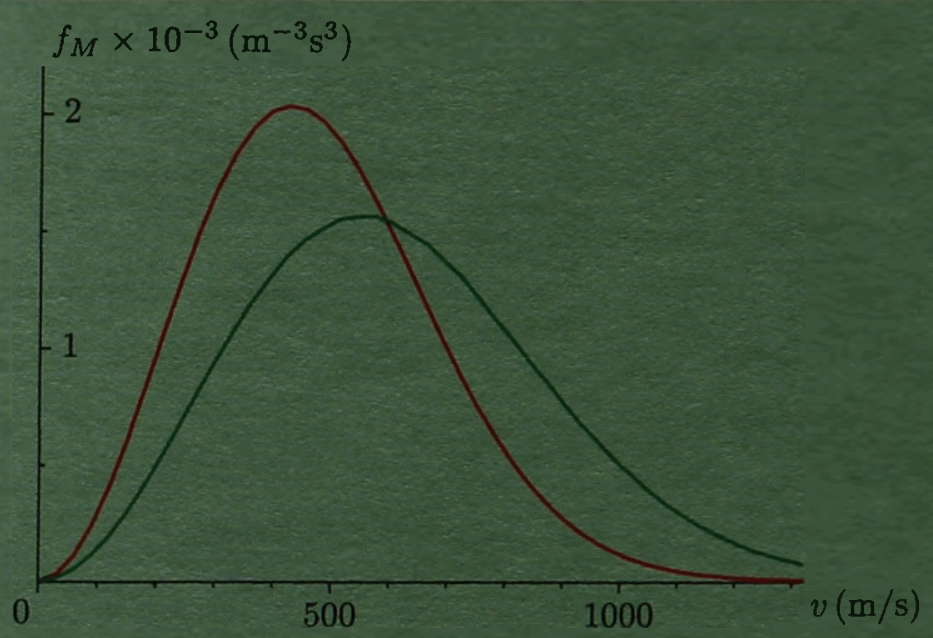
\includegraphics[width=0.4\linewidth]{mai_fig048.png}
   \captionof{figure}{Maxwellovo rozdělení rychlostí molekul dusíku pro teploty \(T_1 = 
                      \SI{300}{\kelvin}\) a \(T_2 = \SI{300}{\kelvin}\).
   \cite[s.~243]{Musilova2009MA1}
   \label{mai:fig048}}
  \par}
  
  Dokážete vyložit, proč jsme zvolili za \(\Delta\Omega\) celý objem slupky? Počítáme totiž 
  pravděpodobnost, že koncový bod vektoru rychlosti molekuly leží, zhruba řečeno, v kterémkoli 
  elementárním kvádříku \(\Delta v_x\Delta v_z\Delta v_z\) obsaženém ve slupce. A ta je součtem 
  pravděpodobností odpovídajících všem kvádříkům vytvářejícím slupku. Jedná se o pravděpodobnosti 
  navzájem neslučitelných jevů (pohybuje-li se molekula v jednom směru, nepohybuje se v jiném). 
  Hustota této pravděpodobnosti se nazývá \textbf{Maxwellovo rozdělení rychlostí}. Na rozdíl od 
  Gaussova rozdělení, popisujícího hustotu pravděpodobnosti pro jednotlivé složky rychlosti, je 
  nesymetrická vlivem faktoru \(v^2\). Obrázek \ref{mai:fig048} ukazuje funkci \(f_M(v)\) pro dvě 
  různé teploty \(T_2 > T_1\). Důležité hodnoty spjaté s tímto rozdělením jsou 
  \textbf{nejpravděpodobnější rychlost} \(v_p\), \textbf{střední rychlost} \(\langle v \rangle\) a 
  \textbf{střední kvadratická rychlost} \(\langle v^2 \rangle\). Platí
  \begin{align*}
    \der{f_M}{v}        &= 0\, \longrightarrow v_P = \sqrt{\dfrac{2kT}{m}},                      \\
    \langle v \rangle   &= \int_{-\infty}^{\infty}vf_M(v)\dd{v} = \sqrt{\dfrac{8kT}{\pi m}},     \\
    \langle v \rangle^2 &= \int_{-\infty}^{\infty}v^2f_M(v)\dd{v} = \dfrac{3kT}{m}.
  \end{align*}
\normalsize
\end{example}
      %---------------------------------------------------------------
  
  \section{Náhoda a zpracování měření}
    \subsection{Součet a součin náhodných veličin}
      Nyní vyřešíme ještě jeden důležitý problém. Víme již, že veličinu \(Y = f(X)\) lze popsat 
      stejnými pravděpodobnostmi jako veličinu \(X\). V řadě případů je však náhodná veličina \(Y\) 
      funkcí několika náhodných veličin \(X_1, X_2, \ldots, X_s\). Každá z nich má nějaké 
      rozdělení. Jaké potom bude rozdělení veličiny \(Y\)? Rozebereme jen dvě základní situace, z 
      nichž je ovšem možné „poskládat“ řadu případů složitějších. Půjde o situace, kdy náhodná 
      veličina bude součtem nebo součinem dvou náhodných veličin, pro jednoduchost značení 
      například \(U\) a \(V\), tedy \(Y = U + V\), \(Z = U \cdot V\). Předpokládejme nejprve, že 
      veličiny \(U\) a \(V\) jsou zcela nezávislé, tj. hodnoty veličiny \(U\) nejsou nijak 
      ovlivněny hodnotami veličiny \(V\) a naopak. Dejme tomu, že \(U\) a \(V\) mají rozdělení
      \begin{equation*}
        \left\lbrace (u_1, p_1), \ldots, (u_k, p_k) \right\rbrace, \qquad
        \left\lbrace (v_1, q_1), \ldots, (v_\ell, v_\ell) \right\rbrace
      \end{equation*}
      Veličiny \(Y = U + V\), resp. \(Z = U \cdot V\) tedy mohou nabývat hodnot \(\lbrace u_i + 
      v_\alpha\rbrace\), resp. \(\lbrace u_i v_\alpha\rbrace\) s pravděpodobnostmi \(p_iq_\alpha\). 
      Jevy \uv{Veličina \(U\) nabude hodnoty \(u_i\)} a \uv{veličina \(V\) nabude hodnoty 
      \(v_\alpha\)} jsou totiž nezávislé. Rozdělení veličin \(Y\) a \(Z\) je 
      \begin{equation*}
        \lbrace (u_i +v_\alpha, p_iq_\alpha)\rbrace,\, \text{resp.}\,
        \lbrace(u_iv_\alpha, p_iq_\alpha)\rbrace,\qquad 1\leq i\leq k,\quad 1\leq\alpha\leq\ell,
      \end{equation*}
      Pro jejich střední hodnoty dostáváme
      \begin{align*}
        \langle y \rangle 
          &= \sum_{i=1}^{k}\sum_{\alpha=1}^{\ell}(u_i + v_\alpha)p_iq_\alpha
           = \sum_{i=1}^{k}u_ip_i\left(\sum_{\alpha=1}^{\ell}q_\alpha\right) + 
             \sum_{\alpha=1}^{\ell}v_\alpha q_\alpha\left(\sum_{i=1}^{k}p_i\right)  \\
          &= \sum_{i=1}^{k}u_ip_i + \sum_{\alpha=1}^{\ell}v_\alpha q_\alpha         \\
        \langle z \rangle 
          &= \sum_{i=1}^{k}\sum_{\alpha=1}^{\ell}(u_i \cdot v_\alpha)p_iq_\alpha
           = \left(\sum_{i=1}^{k}u_ip_i\right)
             \left(\sum_{\alpha=1}^{\ell}v_\alpha q_\alpha\right) 
           = \langle u \rangle \langle v \rangle.
      \end{align*}
      Střední hodnota součtu, resp. součinu náhodných veličin je tedy součtem, resp. součinem jejich
      středních hodnot. Pro součet náhodných veličin platí tento výsledek i v případě, když nebudou
      nezávislé. V tak jednoduchý závěr jsme snad ani nedoufali! Hned uvidíme, jak jej lze využít.
      
      %--Jak číst výsledky studentské ankety aneb není průměr jako průměr----------
      % !TeX spellcheck = cs_CZ
\wikitextrule
\begin{example}\label{mai:exam071}
  \textbf{Jak číst výsledky studentské ankety aneb není průměr jako průměr}\newline\small
  Každý semestr na Masarykově univerzitě se uzavírá vyhodnocením velmi užitečné studentské ankety v 
  Informačním systému MU. Studenti hodnotí na jedenáctihodnotové stupnici (nula až deset bodů) 
  několik položek pro každý studijní předmět (obtížnost, zajímavost, srozumitelnost výkladu, 
  přístup učitele, rozmanitost literatury) a mohou doplnit i slovní komentáře. Na ty se učitelé 
  těší nejvíce, neboť díky anonymitě pisatelů se tak o sobě mohou dovědět leccos zajímavého. 
  Všimneme si však statistického zpracování ankety. U každého předmětu je pro danou položku 
  vypočtena průměrná bodová hodnota odpovědí a vyznačena na téže jedenáctihodnotové stupnici. Pro 
  porovnání je na stupnici vyznačen i takzvaný „fakultní průměr“. Každý přednášející může vidět svá 
  hodnocení a hodnocení svých kolegů, kteří mu vedou cvičení. Děkan má přístupové právo k celé
  statistice, a tak může porovnávat. Jednoho deštivého večera přestalo děkana bavit vyplňování 
  rektorátních formulářů a začal si výsledky ankety prohlížet. Zajímala jej zejména položka 
  „srozumitelnost výkladu“. Řekl si, že všem učitelům, kteří v této položce budou hodnoceni 
  nadprůměrně, zvýší osobní ohodnocení. Soubor předmětů je veliký, a tak děkan klikal a klikal. 
  Zjišťoval, že u veliké většiny předmětů leží průměrné hodnocení srozumitelnosti nad fakultním 
  průměrem. Jeho pocity byly smíšené. Na jedné straně se radoval, jakými jsou jeho podřízení 
  dobrými pedagogy, na druhé straně trnul, kolik to bude stát. Snad aby se raději vrátil 
  k protivným formulářům. Najednou v něm zahlodalo podezření i naděje, že není všechno v pořádku. 
  Jak je možné, že většina hodnocení leží nad průměrem? Kladné a záporné odchylky by se přece měly 
  kompenzovat. Zavolal proto na koberec proděkana pro informační technologie, aby se jej zeptal, co 
  je to „fakultní průměr“. Proděkan odpověděl takto: Máme soubor \(K\) předmětů \(\lbrace 
  X_\alpha\rbrace\), \(\alpha = 1, \ldots, K\). V předmětu \(X_\alpha\) vyplnilo anketu 
  \(N_\alpha\)  studentů, jednotlivé hodnoty odpovědí pro danou položku (srozumitelnost výkladu) 
  byly označeny \(\lbrace x_{\alpha,j}\rbrace\), \(j = 1, \ldots, N_\alpha\). Celkem přirozeně 
  předpokládáme, že váha odpovědi každého studenta je stejná, nezávisle na předmětu. Tato váha je
  rovna převrácené hodnotě celkového počtu studentů, kteří vyplnili anketu, tj. \(w = N^{-1}\), \(N 
  = N_1 + \ldots + N_k\). Fakultní průměr je proto dán vzorcem
  \begin{equation*}
    \langle x \rangle 
      = \sum_{\alpha=1}^{K}\sum_{j=1}^{N_\alpha}wx_{\alpha,j} 
      = \dfrac{1}{N}\sum_{\alpha=1}^{K}\left(\sum_{j=1}^{N_\alpha}x_{\alpha,j}\right)
      = \dfrac{1}{N}\sum_{\alpha=1}^{K}A_\alpha,
  \end{equation*}
  kde jsme označili \(A_\alpha = \sum_{j=1}^{N_\alpha}x_{\alpha,j}\). Děkan chvíli přemýšlel a 
  pravil: To vypadá docela logicky. Neměli bychom však počítat fakultní průměr tak, že vezmeme 
  průměrné hodnoty pro každý předmět a vypočteme jejich aritmetický průměr? Pak bychom dostali
  \begin{equation*}
    \langle \overline{x} \rangle
      = \dfrac{1}{K}\sum_{\alpha=1}^{K}\langle x_{\alpha}\rangle
      = \dfrac{1}{K}\sum_{\alpha=1}^{K}
        \left(\dfrac{1}{N_\alpha}\sum_{j=1}^{N_\alpha}x_{\alpha,j}\right)
      = \dfrac{1}{K}\sum_{\alpha=1}^{K}\dfrac{A_\alpha}{N_\alpha}.
  \end{equation*}
  Tento závěr se akademickým funkcionářům na první pohled nijak zvlášť nelíbil. Bylo totiž jasné, 
  že náhodné veličiny \(X_1, \ldots, X_k\) mají odlišná rozdělení. No jo, řekli si oba, musíme 
  počítat. My už ale počítat nemusíme, neboť jsme takový problém před chvílí vyřešili obecně. 
  Zjistili jsme totiž, že střední hodnota součtu náhodných veličin je rovna součtu středních 
  hodnot, bez ohledu na konkrétní rozdělení každé z veličin. Definujeme-li tedy náhodnou veličinu 
  \(Y\) jako aritmetický průměr veličin \(X_\alpha\), tj.
  \begin{align*}
    Y &= \dfrac{1}{K}\left(X_1 + \ldots + X_K\right),  \\
    \shortintertext{dostaneme}
    \langle y \rangle &= \dfrac{1}{K}\left(\langle x_1 \rangle +\ldots+\langle x_K \rangle\right).
  \end{align*}
  Tento výsledek se shoduje s hodnotou \(\langle \overline{x} \rangle\), kterou pro výpočet 
  „fakultního průměru“ navrhl děkan. Vypočteme-li součet odchylek hodnot \(\langle x_\beta 
  \rangle\) od \(\langle y \rangle\), dostaneme skutečně nulu:
  \begin{equation*}
    \sum_{\beta =1}^{K}\left(\langle x_\beta \rangle - \langle y \rangle\right)
      = \sum_{\beta =1}^{K}\left(\dfrac{A_\beta}{N_\beta} 
      - \dfrac{1}{K}\sum_{\alpha=1}^{K}\langle x_\alpha \rangle\right)
      = 0.
  \end{equation*}
  Zkusme se ještě zamyslet nad tím , jak použití „špatného“ fakultního průměru zkreslilo výsledky a 
  proč. Vypočtěme si rozdíl \(\Delta = \langle \overline{x} \rangle - \langle x \rangle\):
  \begin{equation*}
    \Delta = \langle \overline{x} \rangle - \langle x \rangle 
      = \dfrac{1}{K}\sum_{\alpha=1}^{K}\langle x_\alpha \rangle
      - \dfrac{1}{N}\sum_{\alpha=1}^{K}A_\alpha
      = \dfrac{1}{K}\sum_{\alpha=1}^{K}\langle x_\alpha \rangle
      - \dfrac{1}{N}\sum_{\alpha=1}^{K}N_\alpha\langle x_\alpha \rangle
      = \dfrac{1}{K}\sum_{\alpha=1}^{K}\langle x_\alpha\rangle\left(1 - K\dfrac{N_\alpha}{N}\right).
  \end{equation*}
  Platí přitom
  \begin{equation*}
    \sum_{\alpha=1}^{K}\left(1 - K\dfrac{N_\alpha}{N}\right) = 0.
  \end{equation*}
  Pokud by byl počet studentů, kteří vyplnili anketu, ve všech předmětech stejný, tj. \(N_\alpha = 
  \dfrac{N}{K}\) , byla by odchylka \(\Delta\) podle očekávání nulová. Stejná situace by nastala, 
  kdyby byly shodné všechny průměrné hodnoty \(\langle x_\alpha \rangle\). Je-li odchylka 
  \(\Delta\) kladná, je „nesprávný“ fakultní průměr \(\langle x \rangle\) nižší než \(\langle 
  \overline{x} \rangle\). Proto hodnocení jednotlivých předmětů vypadají příznivěji, právě tak, jak 
  to zjistil děkan. Odchylku \(\Delta\) posouvají do kladných hodnot předměty, které hodnotilo málo 
  studentů, a předměty, které měly vysoké hodnocení. Dobře je to vidět na příkladu dvou předmětů, 
  tj. pro \(K = 2\), kde vychází
  \begin{equation*}
    \Delta = \langle \overline{x} \rangle - \langle x \rangle 
           = \dfrac{N_2 - N_1}{2(N_2+N_1)}\left(\langle\overline{x}\rangle-\langle x\rangle\right).
  \end{equation*}
  
  Pro \(N_1\ll N_2\) a \(\langle x_1 \rangle  \gg \langle x_2 \rangle \) bude rozdíl \(\Delta\) 
  skoro polovina hodnoty \(\langle x_1 \rangle\)! U volitelných specializovaných předmětů, které si 
  vybírají jen poměrně malé počty studentů, kteří navíc mají o předmět opravdový zájem a hodnotí 
  jej proto většinou vyšším počtem bodů, je splněno obojí (malý počet hodnotících a vysoké bodové
  hodnocení). Je vidět, že při nesprávně zvoleném výpočtu srovnávací hodnoty (fakultního průměru) 
  mohou právě předměty, jejichž statistický význam je spíše okrajový, ovlivnit celkové hodnocení.
\normalsize
\end{example}
      %----------------------------------------------------------------------------
      
      Pro střední hodnotu součtu a součinu nezávislých náhodných veličin jsme získali velmi
      jednoduché výsledky:
      
      \adjustbox{minipage=[c]{\textwidth}}{%
        \begin{equation}\label{mai:eq070}
          \langle u + v \rangle = \langle u \rangle + \langle v \rangle\qquad
          \langle uv \rangle    = \langle u \rangle \langle v \rangle.
        \end{equation}
      }
      
      Dokážeme také určit rozptyl veličin \(Y = U + V\) a \(Z = U\cdot V\)? Pro rozptyl každé 
      náhodné veličiny platí obecný vztah (\ref{mai:eq061}). Použijeme jej pro naše konkrétní 
      případy:
      \begin{align*}
        D(U + V) &= \langle (u + v)^2 \rangle - \langle u + v \rangle^2 
                  = \langle u^2 + 2uv + v^2 \rangle - \left(\langle u \rangle^2 +
                    \langle 2uv \rangle + \langle v^2 \rangle\right)                        \\
                 &= \left(\langle u^2\rangle - \langle u \rangle^2\right)
                  + \left(\langle v^2\rangle - \langle v \rangle^2\right) = D(U) + D(V).
      \end{align*}
      Pro rozptyl náhodné veličiny \(Z = U \cdot V\) dostaneme
      \begin{align*}
        D(Z)  &= \langle z^2\rangle - \langle z \rangle^2 
               = \langle u^2\rangle\langle v^2\rangle - \langle u \rangle^2 \langle v \rangle^2  \\
              &= \left[D(U) + \langle u^2\rangle\right]\left[D(V) + \langle v^2\rangle\right]
               - \langle u \rangle^2 \langle v \rangle^2                                         \\
              &= D(U)D(V) + \langle u \rangle^2D(V) + \langle v \rangle^2D(U).
      \end{align*}
      Pak
      \adjustbox{minipage=[c]{\textwidth}}{%
        \begin{equation*}
          \dfrac{D(z)}{ \langle z \rangle^2} = \dfrac{D(U)}{ \langle u \rangle^2} \cdot
            \dfrac{D(V)}{ \langle v \rangle^2} + \dfrac{D(U)}{ \langle u \rangle^2} +
            \dfrac{D(v)}{ \langle v \rangle^2}.
        \end{equation*}
      }
      Při výpočtu jsme využili vztahu (\ref{mai:eq061}) a vztahů (\ref{mai:eq070}) pro střední 
      hodnotu součtu a součinu náhodných veličin. Pokud mají veličiny \(U\) a \(V\) shodný rozptyl 
      \(D(U) = D(V) = D\), pak je \(D(U + V) = 2D\). V případě součtu s veličin \(Y = X_1 + \cdots 
      + X_s\) se shodným rozptylem \(D\) resp. směrodatnou odchylkou \(\sigma\) dostáváme
      \begin{equation*}
        D(Y) = sD  \Rightarrow \sigma(y) = \sqrt{s}\sigma.
      \end{equation*}
      Znovu připomeňme, že všechny vztahy týkající se součtu a součinu náhodných veličin, které
      jsme zatím získali, platí za předpokladu, že výchozí veličiny, které sčítáme nebo násobíme, 
      jsou nezávislé.
      
      Aniž bychom se podrobněji zabývali vlastnostmi rozdělení závislých veličin, definujeme pro
      ně charakteristiky, které tuto závislost popisují. Nechť \(U\) a \(V\) jsou dvě libovolně 
      náhodné veličiny, ne nutně nezávislé. Míru jejich závislosti určují veličiny
      \begin{equation}\label{mai:eq071}
        \sigma_{uv} = \langle (u - \langle u \rangle) (v - \langle v \rangle) \rangle, \qquad
        \varrho_ {uv}=\dfrac{\sigma(u)}{\sqrt{D(U)D(V)}} = \dfrac{\sigma(u)}{\sigma{D(u)\sigma(v)}}
      \end{equation}
      zvané \textbf{kovariance} a \textbf{korelační koeficient} veličin \(U\) a \(V\). Platí 
      \(\varrho(uv) \leq 1\). Pro nezávislé veličiny vychází \(\sigma(uv) = 0\) a \(\varrho(uv) = 
      0\).
      
      %-- Rozptyl při Bernoulliově pokusu-----------------------------
      % !TeX spellcheck = cs_CZ
\begin{mdframed}[style=mdexam]
  \begin{example}\label{mai:exam072}
    \textbf{Rozptyl při Bernoulliově pokusu}\newline
    V příkladu \ref{mai:exam066} jsme se zajímali o střední hodnotu veličiny \(X\) definované jako
    počet zdarů při \(n\) opakováních Bernoulliova pokusu. Řekli jsme si, že střední hodnota této
    veličiny je \(np\) s tím, že důkaz lze provést přímo na základě definičního vztahu pro střední
    hodnotu matematickou indukcí. Výpočet rozptylu z definičního vztahu bychom jistě snadno dokázali
    zahájit, horší by však bylo dovést jej do konce. Stačí se podívat na začátek výpočtu
    \begin{align*}
      D(X) &= \sum_{j=0}^n \left(x_j - \langle x \rangle\right)^2p_j             \\
           &= \sum_{j=0}^n \left(j - np\right)^2\binom{n}{j}p^j(1 - p)^j,
    \end{align*}
    a nepochybujeme o tom, že tuto sumu nedokážeme spočítat snadno. Protože již však umíme zacházet
    se součtem náhodných veličin, můžeme využít účinného triku. Veličinu \(X\) si představíme jako
    součet
    \begin{equation*}
      X = U_1 + U_2 + \cdots + U_n,
    \end{equation*}
    kde každá z veličin \(U_j\) může nabývat dvou hodnot. Jedničky v případě, že při \(j\)-tém
    opakování pokusu nastal zdar, a nuly v případě, že nastal nezdar. Součet všech veličin \(U_j\)
    pro \(j = 1\) až \(j = n\) pak skutečně znamená celkový počet zdarů při \(n\) opakováních
    pokusu. Jestliže si uvědomíme, že pravděpodobnost zdaru při kterémkoli z opakování je \(p\) a
    pravděpodobnost nezdaru \((1 - p)\), ihned vidíme, že rozdělení každé z veličin \(U_j\) má tvar
    \(\lbrace(1, p), (0, 1 - p)\rbrace\). Platí tedy
    \begin{equation*}
      \langle u_j\rangle = 1\cdot p + 0 \cdot (1 - p) = p,
    \end{equation*}
    \begin{align*}
      D = D(U_j) &= \left( 1 - \langle u_j\rangle\right)^2p 
                  + \left( 0 - \langle u_j\rangle\right)^2(1 - p)   \\
                 &= p(1 - p)^2 + p^2(1 - p) = p(1 - p).
    \end{align*}
    Každé dvě veličiny \(U_i\), \(U_j\) jsou nezávislé, neboť jednotlivá opakování pokusu jsou
    nezávislá. Střední hodnota jejich součtu je: tedy \(np\) (a to souhlasí s informací v příkladu
    \ref{mai:exam066}) a pro rozptyl jejich součtu platí
    \begin{equation*}
      D(X) = nD = np(1 - p).
    \end{equation*}
    Celkově tedy dostáváme
    \begin{equation*}
      \langle x \rangle = np, \; \sigma(x) = \sqrt{np(1 - p)}.
    \end{equation*}
  \end{example}
\end{mdframed}
      %---------------------------------------------------------------
      
      %-- Rozptyl aritmetického průměru-------------------------------
      % !TeX spellcheck = cs_CZ
\begin{mdframed}[style=mdexam]
  \begin{example}\label{mai:exam073}
    \textbf{Rozptyl aritmetického průměru}\newline
    Již v úvodu odstavce o náhodných veličinách jsme konstatovali, že opakujeme-li v nezměněných
    podmínkách měření jisté fyzikální veličiny (délka závěsu kyvadla, proud procházející vodičem,
    napětí na vodiči, atd.), budeme díky náhodným vlivům dostávat pokaždé poněkud jiný výsledek.
    Říkáme, že měření je zatíženo náhodnými chybami. Výsledek získaný při každém opakování lze
    interpretovat jako hodnotu náhodné veličiny. Dejme tomu, že jsme provedli uměření fyzikální
    veličiny \(X\) a získali hodnoty \(x_1\) až \(x_n\) . V praktické situaci budou tyto hodnoty
    většinou navzájem různé, nemusí tomu tak však nutně být. Fyzikální veličinu chceme ovšem
    reprezentovat jediným údajem, a tím bude její střední hodnota, tj.
    \textbf{aritmetický průměr}
    \begin{equation*}
      \langle x \rangle = \dfrac{x_1 + x_2 + \cdots + x_n}{n}.
    \end{equation*}
    Rozptyl veličiny \(X\) je dán vztahem
    \begin{align*}
      D &= D(X)                                                             \\
        &= \dfrac{\left(x_1 - \langle x \rangle\right)^2 + 
                  \left(x_2 - \langle x \rangle\right)^2 + \cdots +
                  \left(x_n - \langle x \rangle\right)^2}{n}.
    \end{align*}
    Víme, že směrodatná odchylka \(\sigma( x ) = \sqrt{D(X)}\) určuje, nakolik jsou jednotlivé
    výsledky měření v průměru odchýleny od střední hodnoty, charakterizuje tedy přesnost každého
    opakování měření. Podívejme se na celou úlohu z jiné strany: Představme si, že sledujeme \(n\)
    po dvou nezávislých náhodných veličin \(X_1\) až \(X_n\) se shodnou střední hodnotou \(\langle
    x_j \rangle = \langle x \rangle\) a shodnou směrodatnou odchylkou \(\sigma(x_j) = \sqrt{D},\, 1
    \leq j \leq n\). Aritmetický průměr těchto veličin,
    \begin{equation*}
      \langle \Xi \rangle = \dfrac{X_1 + X_2 + \cdots + X_n}{n}.
    \end{equation*}
    je tedy rovněž náhodnou veličinou. Pro jeho střední hodnotu, rozptyl a směrodatnou odchylku
    platí
    \begin{align*}
      \langle \xi \rangle 
                  &= \dfrac{n\langle x \rangle}{n}, \\
      D(\Xi)      &= \dfrac{1}{n^2}\cdot D(X_1 + \cdots + X_n)=\dfrac{nD^2}{n^2}=\dfrac{D}{n}, \\
      \sigma(\xi) &= \dfrac{\sigma(x)}{\sqrt{n}}.
    \end{align*}
  \end{example}
\end{mdframed}
      %---------------------------------------------------------------
      
      Můžeme tedy říci, že aritmetický průměr všech výsledků měření dané fyzikální veličiny je
      \(\sqrt{n}\)-krát přesnější než jednotlivý výsledek měření. Jakkoli se toto konstatování zdá 
      intuitivně zřejmé, je třeba je používat s opatrností.
      
      Především je třeba mít na mysli, co toto konstatování znamená. Jeho charakter je totiž
      opět jen pravděpodobnostní. Jestliže jsou jednotlivá měření prováděna za stejných podmínek,
      jsou rozdělení veličin \(X_1\) až \(X_n\) funkcemi téhož typu. Tyto veličiny mají také 
      stejnou střední hodnotu \(\langle x \rangle\) a směrodatnou odchylku \(\sigma\). Také 
      pravděpodobnost, že při měření padne hodnota veličiny \(X_j\) do intervalu \((\langle x 
      \rangle - \sigma, \langle x \rangle + \sigma)\), je pro všechna \(j\) prakticky stejná. 
      Označme ji \(P_\sigma\).  Se stejnou pravděpodobností nabude aritmetický průměr \(\Xi\) 
      hodnoty v intervalu určeném svou směrodatnou odchylkou. Ta je však \(\sqrt{n}\)-krát menší. V 
      tomto smyslu jsou hodnoty aritmetického průměru \uv{\(\sqrt{n}\)-krát méně rozptýleny} kolem 
      střední hodnoty \(\langle\xi \rangle\) než hodnoty náhodných veličin \(X_j\) kolem svých 
      středních hodnot \(\langle x \rangle\).
      
      Dalším problémem může být splnění výchozích předpokladů, které vedly ke vztahu pro
      směrodatnou odchylku aritmetického průměru. Ukážeme to na následujícím příkladu.
      
      %-- Jak přesně lze změřit čínského císaře?----------------------
      % !TeX spellcheck = cs_CZ
\wikitextrule
\begin{example}\label{mai:exam075}
  \textbf{Ověření Ohmová zákona}\newline\small

\normalsize
\end{example}
      %---------------------------------------------------------------
      
      %-- Záhada přijímací zkoušky aneb k čemu může posloužit distribuční funkce-----
      % !TeX spellcheck = cs_CZ
\begin{mdframed}[style=mdexam]
  \begin{example}\label{mai:exam075}
    \textbf{Záhada přijímací zkoušky aneb k čemu může posloužit distribuční funkce?}\newline
    Mohlo by se zdát, že distribuční funkce je jen teoretický pojem a že v praktických situacích ji
    těžko využijeme. Podstatné je přece pravděpodobnostní rozdělení náhodné veličiny a distribuční
    funkce je z něj jen jaksi odvozena sčítáním pravděpodobností (u diskrétního rozdělení) nebo
    integrací (u rozdělení spojitého). Přesvědčíme se, že existují velmi realistické případy, kdy
    distribuční funkce přináší věrohodnější informaci o náhodné veličině než samotné rozdělení.
    
    Na Masarykově univerzitě musí každý uchazeč o studium, ať již se hlásí na přírodovědeckou,
    právnickou, lékařskou či jinou fakultu, absolvovat Test studijních předpokladů. Jedná se o
    všeobecný test, zaměřený na zjišťování úrovně všech schopností uchazeče, které jsou potřebné pro
    univerzitní studium, například analytického myšlení, verbálních schopností, numerického myšlení,
    geometrické představivosti, atd. Pro nás však v tu to chvíli není podstatný obsah testu, ale
    způsob zpracování jeho výsledků a vyhodnocení pořadí uchazečů. Test skládá kolem třiceti tisíc
    studentů. Není tedy možné technicky zajistit, aby proběhl v jediné variantě v jednom dni. K
    dispozici je proto osm variant testu, každou variantu řeší tři až čtyři tisíce studentů. Test má
    \num{80} otázek, základním údajem pro zpracování jeho výsledků je počet správných odpovědí
    každého studenta. Pokud bychom označili jako \(i\) počet správných odpovědí (\(i \in\lbrace0, 1,
    2, \ldots, 80\rbrace\)) v kterékoli variantě a \(\mathcal{N}_i\) počet studentů, kteří dosáhli
    právě \(i\) správných odpovědí, dostaneme náhodnou veličinu \(X_i\), kterou bychom mohli nazvat
    „počet správných odpovědí“, pro celou univerzitu. Její rozdělení by mělo tvar
    \begin{equation*}
      \lbrace(i,p_i)\rbrace,\quad\text{kde}\qquad p_i = \dfrac{\mathcal{N}_i}{\mathcal{N}}, \quad
      \mathcal{N} = \sum_{i=0}^{80}\mathcal{N}_i
    \end{equation*}
    A zde je malý „kámen úrazu“. A by bylo možné sestavit opravdu „univerzální pořadí“, musely by
    být všechny varianty testu ekvivalentní z hlediska obtížnosti. To znamená, že kdyby kterýkoli
    student vyplnil za stejných podmínek všechny varianty, dosáhl by v každé z nich stejného počtu
    správných odpovědí s pravděpodobností velmi blízkou jedné. Skutečnost je však principiálně
    taková, že u sebelépe promyšleného a sestaveného testu se jednotlivé varianty budou mírně, v
    rámci statistických, a tedy již neodstranitelných, odchylek lišit. Tato odlišnost se nepozná
    předem, ale až po zpracování výsledků všech variant. Použít pro stanovení pořadí uchazečů
    rozdělení náhodné veličiny \(X\) \emph{= počet správných odpovědí je tedy nespravedlivé}.
    Student, který řešil variantu „statisticky obtížnější“, by v pořadí skončil s horším umístěním,
    než student, který je stejně schopný, avšak měl to štěstí, že na něj připadla varianta
    „statisticky méně obtížná“. Skutečně, kdybychom sestavili grafy rozdělení náhodných veličin
    \(X^{(\alpha)}\) \emph{= počet správných odpovědí v \(\alpha\)-té variantě},
    \begin{equation*}
      \lbrace(i,p_i^{(\alpha)})\rbrace,\quad\text{kde}\; 
      p_i^{(\alpha)} = \dfrac{\mathcal{N}_i^{(\alpha)}}{\mathcal{N}^{(\alpha)}}, \quad
      \mathcal{N}^{(\alpha)} = \sum_{i=0}^{80}\mathcal{N}_i^{(\alpha)}
    \end{equation*}
    zjistili bychom, že se mírně liší. (V předchozím zápisu značí \(\mathcal{N}_i^{(\alpha)}\) počet
    studentů, kteří odpověděli správně na \(i\) otázek \(\alpha\)-té varianty
    \(\mathcal{N}^{(\alpha)}\) je počet všech studentů, kteří tuto variantu řešili.) Střední hodnoty
    i mediány náhodných veličin se i při vynikající shodě obtížnosti všech variant mohou lišit v
    rozmezí jedné až dvou správných odpovědí. A s ohledem na skutečnost, že každou variantu řeší
    obrovský počet studentů, až čtyři tisíce, je zřejmé, že tento rozdíl může poněkud „zamíchat
    “pořadím, zejména v blízkosti mediánu, kde se týká třeba i tří stovek studentů v každé variantě.
    Situaci dokládá obrázek \ref{mai:fig049}. Jak tedy zařídit, abychom dostali spravedlivé pořadí?
    Jediný rozumný způsob, jak minimalizovat vliv statistických odchylek obtížnosti jednotlivých
    variant, je nehodnotit studenty podle absolutního počtu správných odpovědí, ale nějak je
    porovnat mezi sebou. Budeme při tom předpokládat, že rozložení schopností studentů je ve všech
    osmi skupinách, které řeší osm daných variant, stejné. Řeknete si - zase nějaké další
    předpoklady. To je jako z bláta do louže. Předpoklad o stejném rozložení schopností studentů v
    tak velkých skupinách, jako jsou ty naše, je však mnohem realističtější než předpoklad o
    dokonalé shodě obtížnosti variant testu. Budeme se jej proto držet. Každému studentovi
    přisoudíme číslo, které informuje o tom, kolik řešitelů dané varianty bylo horších nebo stejně
    dobrých jako on, tj. mělo nižší nebo stejný počet správných odpovědí. Z matematického hlediska
    to znamená přejít v každé variantě od rozdělení k distribuční funkci. Věnujme se nyní tomuto
    přepočtu podrobněji jak pro diskrétní rozdělení náhodné veličiny \(X^{(\alpha)}\), které
    odpovídá skutečné situaci, tak pro zajímavost i pro rozdělení spojité. V dalším budeme vždy
    zpracovávat výsledky jedné varianty, upustíme proto od vyznačování indexu \(\alpha\).

    {\centering
    \captionsetup{type=figure}
    \luafigure[0.8]{mai_fig049.png}
    \captionof{figure}{Rozdělení pro dvě varianty testu,
    \cite[s.~252]{Musilova2009MA1}
    \label{mai:fig049}}
    \par}
    
    \textbf{Diskrétní rozdělení}
      \begin{itemize}
        \item \emph{Zadání:} Skupina \(N\) studentů řeší jednu variantu testu. Test má \(Q\) otázek.
              Za každou správnou odpověď je přidělen jeden výchozí bod. Získáváme rozdělení
              \begin{gather*}
                \left\lbrace\left(i, \dfrac{N_i}{N} \right)\right\rbrace, \;
                i\in\lbrace0, 1, 2, \ldots, Q\rbrace, \;
                \sum_{i=0}^{Q}N_i = N 
              \end{gather*}
              kde \(i\) je počet výchozích bodů a \(N_i\) počet studentů, kteří získali \(i\) bodů.
              Distribuční funkce tohoto rozdělení
              \begin{gather*}
                F(x) = \dfrac{1}{N}\sum_{i=0}^{j}N_i\;\text{ pro }\;
                j\leq x < j+1, \; x\in\left[0,\infty\right)
              \end{gather*}
              Pro uchazeče, který získal \(j\) bodů, mají význam následující hodnoty:
              \begin{itemize}
                \item \(F(x)    x \in \left[j, j+1\right)\): poměrný počet uchazečů, kteří získali
                      počet výchozích bodů nižší nebo shodný s daným uchazečem,
                \item \(NF(x)   x \in \left[j, j+1\right)\): absolutní počet uchazečů, kteří získali
                      počet výchozích bodů nižší nebo shodný s daným uchazečem,
                \item \(100F(x) x \in \left[j, j+1\right)\): absolutní počet uchazečů, kteří získali
                      počet výchozích bodů nižší nebo shodný s daným uchazečem,
              \end{itemize}
        \item Hodnoty distribuční funkce můžeme získat z následující tabulky:
        
              {\centering
                \resizebox{0.8\textwidth}{!}{%
                \begin{tabular}{c|c}
                          interval \(x\)     &  \(NF(x)\)         \\ \hline
                  \(\left[0,1\right)\)       &  \(N_0\)           \\ 
                  \(\left[1,2\right)\)       &  \(N_0 + N_1\)     \\ 
                  \(\cdots\)                 &  \(\cdots\)        \\
                  \(\left[j,j+1\right)\)     &  \(N_0 + N_1 + \cdots + N_j\) \\ 
                  \(\cdots\)                 &  \(\cdots\) \\
                  \(\left[Q-1,Q\right)\)     &  \(N_0 + N_1 + \cdots + N_{Q-1}\) \\ 
                  \(\left[Q,\infty\right)\)  &  \(N_0 + N_1 + \cdots + N_{Q} = N\) 
                \end{tabular}}
              \par}
        \item Přepočet hodnocení uchazečů tak, aby nová stupnice byla opět v rozsahu mezi nulou a
              \(Q\) a aby nové hodnocení bylo opět celočíselné, je následující:
              \begin{equation*}
                y =QF(x), \quad 0\leq F(x) \leq 1, \Rightarrow y \in[0,Q].
              \end{equation*}
              Uchazeči se ziskem \(i\) výchozích bodů náleží hodnota \(y = QF(x)\) právě když i\(
              \in \left[i, i + 1\right)\), tj. \(y_i = Q F(i)\). Tato hodnota není obecně
              celočíselná. Zaokrouhlení se provede ve prospěch uchazeče, tedy vždy nahoru. Výsledný
              převodní vzorec je
              \begin{equation*}
                \begin{multlined}
                  \text{výchozí body } i \longrightarrow\text{ nové body }  \\ 
                  \shoveleft[1cm]Y_i: Y_i = [y_i] + 1 = [QF(i)] + 1,
                \end{multlined}
              \end{equation*} 
              kde \([a]\) značí celočíselnou část čísla \(a\), tedy například \([\num{23.05}] =
              [\num{23.48}] = [23,89] = 23\)
        \item Zaveďme novou náhodnou veličinu \(Z\) s rozdělením \(\left\lbrace(z_\alpha,
              M_\alpha)\right\rbrace\): Označme \(z_1, z_2, \ldots, z_\alpha, ...,\) \(z_S\)
              navzájem různé hodnoty ze souboru \(\lbrace Y_i\rbrace, i = 0, 1, 2, \ldots, Q\)
              řazené vzestupně. Její rozdělení udává kterákoli z následujících tabulek:

              {\centering
                \resizebox{0.9\textwidth}{!}{%
                \begin{tabular}{c|c}
                          hodnota                       &  četnost         \\
                          \hline
                  \(z_1 = Y_0 = Y_1 = \cdots Y_{i_1}\)  & \(M_1 = N_0 + N_1 + \cdots + N_{i_1}\)  \\ 
                  \(Z_2 = Y_{i_1+1} = \cdots Y_{i_2}\)  & \(M_2 = N_{i_1+1} + \cdots + N_{i_2}\)  \\ 
                  \(\cdots\)                            & \(\cdots\)                              \\
                  \(Z_S = Y_{i_{S-1}+1}=\cdots Y_{i_S}\)& \(M_S = N_{i_{S_1}+1}+\cdots+N_{i_S}\)   
                \end{tabular}}
              \par}

              {\centering
                \resizebox{0.9\textwidth}{!}{%
                \begin{tabular}{c|c}
                          hodnota                        &  četnost         \\
                          \hline
                  \(z_1 = Y_0 = Y_1 = \cdots Y_{i_1}\)   &  \(M_1 = NF(i_1)\)              \\
                  
                  \(Z_2 = Y_{i_1+1} = \cdots Y_{i_2}\)   &  \(M_2 = N[F(i_2) - F(i_1)]\)  \\ 
                  \(\cdots\)                             &  \(\cdots\)                     \\
                  \(Z_S = Y_{i_{S-1}+1}=\cdots Y_{i_S}\) & \(M_S = N[F(i_S) - F(i_{S-1})]\)   
                \end{tabular}}
              \par}
              kde \(i_1 < i_2 < \ldots < i_{S-1} < i_S, i_S = Q\) (Vzhledem k zaokrouhlování nahoru
              není žádná bodová hodnota \(Y_i\) nulová.) I když skutečné rozdělení při zpracování
              výsledků testů je diskrétní, ukažme si, jak by vypadal analogický postup u rozdělení
              spojitého, kde je početní zpracování názornější.
      \end{itemize}
    
    \textbf{Spojité rozdělení}
      \begin{itemize}
        \item \emph{Zadání:} Je dáno rozdělení četností \(n(x) \leq 0,\, x \in [0, Q]\).
        \item Normovací podmínka a distribuční funkce jsou
              \begin{equation*}
                \int_{0}^{Q}n(x)\dd{x} = N, \quad 
                F(x) = \dfrac{1}{n}\int_{0}^{x}n(\xi)\dd{\xi},                
              \end{equation*}
              kde \(0 \leq F(x) \leq 1.\)
        \item Označme \(z = QF(x)\), tedy \(z \in [0, Q]\), novou náhodnou veličinu. (Uvědomme si,
              že \(z\) je rostoucí funkcí proměnné \(x\)). Označme její rozdělení \(\nu(z)\). Její
              distribuční funkce je
              \begin{align*}
                \Phi(z) &= \int_{0}^{z}\nu(\zeta)\dd{\zeta} 
                         = \int_{0}^{x(z)}\dfrac{n(\xi)}{N}\dd{\xi}          \\
                        &= F\left(F^{-1}(z/Q)\right) 
                        = \dfrac{z}{Q}, \quad
                \nu(z) = \dfrac{1}{Q}.
              \end{align*}
        \item Rozdělení je konstantní s mediánem i střední hodnotou \(Q/2\). Takové rozdělení se
              nazývá rovnoměrné.
      \end{itemize}
  \end{example}
\end{mdframed}
      %------------------------------------------------------------------------------
      
    \subsection{Který výsledek je ten pravý?}
      První věc, kterou budete dělat ve fyzikálním praktiku, bude zjišťování průměrné hustoty 
      materiálu, z něhož je vyroben kovový váleček. Budete váleček vážit, abyste určili jeho 
      hmotnost,a měřit jeho výšku a průměr, abyste mohli vypočítat jeho objem. Hustotu stanovíte 
      jako podíl hmotnosti a objemu. Jedná se stále o jeden a týž váleček, jehož průměrná hustota 
      má za daných podmínek (stálá teplota, váleček se nedeformuje, apod.) stále stejnou „správnou“ 
      hodnotu, kterou však neznáme. (Nezná ji ani učitel v praktiku, i když se tak tváří.) Změří-li 
      hustotu válečku všichni studenti ve skupině, každý jen jednou, získá se řada různých hodnot. 
      Která z nich je ta správná? Není vyloučeno, a je to dokonce velmi pravděpodobné, že žádná. A 
      mohli bychom pomocí nich správnou hodnotu určit nebo se k ní alespoň přiblížit? Možné by to 
      bylo, pokud bychom zaručili, že všechny výsledky získané jednotlivými studenty jsou „stejně 
      hodnotné“. Znamenalo by to, že bychom museli vyloučit hrubé a systematické chyby, které by 
      vznikly třeba tak, že by někteří studenti vážili na vadných vahách, někteří by měli špatné 
      měřítko, popřípadě by odečítali údaj „zboku“, takže by byl zkreslený, nebo by se dokonce 
      zmýlili při odečítání údaje. Museli bychom také zaručit, že náhodné vlivy, které ovlivňují 
      měření, zatěžují je náhodnými chybami a v principu je nelze odstranit, byly při všech 
      měřeních stejné. U různých studentů si tím však nemůžeme být jisti (vzpomeňte si na měření 
      čínského císaře), proto budeme raději postupovat tak, že jeden pečlivý student provede větší 
      počet měření třeba výšky válečku, která je pro určení hustoty potřebná. Dejme tomu, že bude 
      měřit milimetrovým měřítkem a bude odhadovat s přesností na půl milimetru. Jeho údaje tedy 
      mohou mít tvar \SI{33.0}{\mm}, \SI{34.5}{\mm}, atd. Získá takto za stejných podmínek třeba 
      dvacet nebo i padesát hodnot, ale co teď s nimi? Jak určit hodnotu, která se bude nejvíce 
      blížit správné hodnotě výšky válečku? (Dalo by se jistě diskutovat i o tom, co je to správná 
      hodnota. Pro tuto chvíli však předpokládejme, že taková hodnota skutečně existuje, neboť 
      váleček je opravdu válcem, je vysoustružen pečlivě, přesněji, než jsme schopni jej měřit, při 
      měření se nemění teplota, váleček není dáván do lisu a deformován, ani upravován tak, že by 
      se měnila jeho hmotnost.) Předpokládejme, že správná hodnota výšky válečku je \(x\) a že 
      student naměřil hodnoty \(\lbrace x_1, X_2, \ldots, x_n\rbrace\), mezi nimiž mohou být 
      pochopitelně i některé hodnoty stejné. Odchylky jeho měření od správné hodnoty jsou
      \begin{equation*}
        \lbrace \varepsilon_1, \varepsilon_2, \ldots, \varepsilon_n\rbrace, \qquad
        \varepsilon_i = x_i - x, \qquad i = 1, 2, \ldots, n.
      \end{equation*}
      I kdybychom správnou hodnotu \(x\) znali, nedokázali bychom předpovědět, nakolik se od ní při
      jednotlivém měření odchýlíme. Můžeme, se však zajímat o to, jaká je pravděpodobnost, že
      hodnota, o kterou bude měření od správné hodnoty odkloněno, bude ležet v určitém intervalu.
      Odchylky \(\varepsilon_i\) lze totiž interpretovat jako hodnoty náhodné veličiny. Abychom 
      mohli požadované pravděpodobnosti určit, potřebujeme znát rozdělení této veličiny. Označme ji 
      \(\varepsilon\) a odpovídající hustotu pravděpodobnosti \(\mathcal{w}(\varepsilon)\). Toto 
      rozdělení je za určitých podmínek \textbf{rozdělením normálním}, splňuje tedy vztah 
      (\ref{mai:eq069}). Zkusme se o tom přesvědčit. Zvolme podmínky měření tak, aby byly ve hře 
      jen náhodné chyby způsobené \(m\) nezávislými vlivy. Každý z nich hodnotu měření
      odchýlí od \(x\) o stejně velkou hodnotu \(\alpha\), kladnou nebo zápornou, s 
      pravděpodobností \num{0.5}. Schéma této úvahy je na obrázku \ref{mai:fig050}. Výsledná 
      odchylka naměřené hodnoty \(x_i\) od hodnoty správné s jistotou leží v intervalu \((-m\alpha, 
      m\alpha)\) a může nabývat pouze hodnot celých násobků \(\alpha\). Při uplatnění jednotlivého 
      „chybového“ vlivu vzniká, jak jsme již řekli, kladná nebo záporná odchylka o velikosti 
      \(\alpha\). Vznik odchylky \(+\alpha\) nazveme zdarem, vznik odchylky \(-\alpha\) nezdarem.
      
      \begin{figure}[ht!] %\ref{mai:fig050}
        \centering
        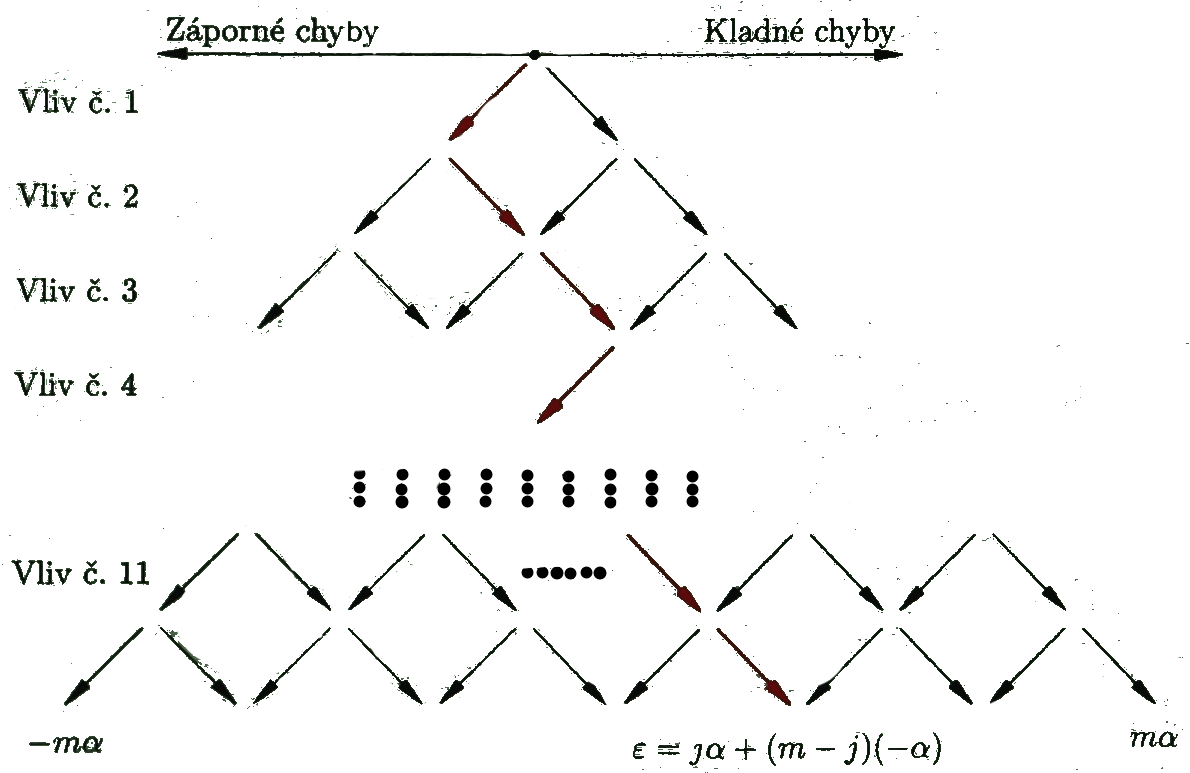
\includegraphics[width=0.6\linewidth]{mai_fig050.png}
        \caption{Vznik kladných a záporných odchylek při měření s \(m\) vlivy. 
        \cite[s.~255]{Musilova2009MA1}}
        \label{mai:fig050}
      \end{figure}
      
      Mohlo by tomu být i naopak, slova „zdar“ a „nezdar“ zde nemají svůj obvyklý význam, jde
      pouze o to, že díky nim můžeme hned uvidět souvislost s Bernoulliovým pokusem a tedy
      i s Bernoulliovým rozdělením. Při \(j\) kladných a \(m — j\) záporných odchylkách je měření od
      správné hodnoty odkloněno o
      \begin{equation*}
        j\alpha + (m - j)(-\alpha) = (2j - m)\alpha
      \end{equation*}
      s pravděpodobností
      \begin{equation*}
        p_j = \begin{pmatrix}m j\end{pmatrix}p^j(1 - p)^{m - j} = 2^{-m}.
      \end{equation*}
      Střední hodnota náhodné veličiny \(\varepsilon\) je nulová. Skutečně, v příkladu 
      \ref{mai:exam066} jsme zjistili, že střední hodnota veličiny \(Y\) nabývající hodnot \(y_j = 
      j\) s Bernoulliovým rozdělením je \(\langle y \rangle = mp\), střední hodnota veličiny \((2j 
      — m)\) a pak musí být \((2mp — m)\alpha\). Pro \(p = \num{0.5}\) je tato hodnota nulová.
      Pro velká \(m\) lze Bernoulliovo rozdělení nahradit rozdělením normálním (obr. 3.8), a proto 
      má náhodná veličina \(\varepsilon\) hustotu pravděpodobnosti tvaru (\ref{mai:eq069}), tj.
      \begin{equation*}
        \mathcal{w}(\varepsilon) = 
        \dfrac{1}{\sigma\sqrt{2\pi}}\exp\left(\dfrac{-\varepsilon^2}{2\sigma^2}\right).   
      \end{equation*}
      \begin{figure}[ht!] %\ref{mai:fig051}
        \centering
        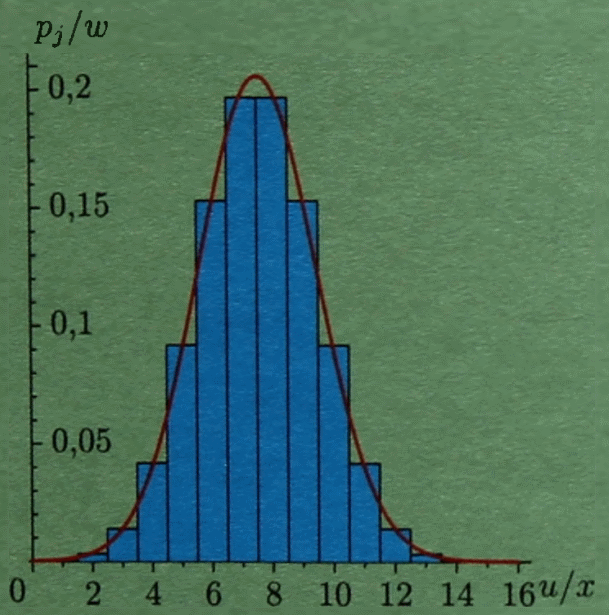
\includegraphics[width=0.4\linewidth]{mai_fig051.png}
        \caption{Normální rozdělení jako limitní případ Bernoulliova 
        \cite[s.~256]{Musilova2009MA1}}
        \label{mai:fig051}
      \end{figure}
      
      Vraťme se nyní k otázce zpracování naměřených hodnot \(\lbrace x_1, \ldots, x_n\rbrace\) 
      výšky válečku. Jejich odchylky od správné hodnoty jsou \(x_1 - x\) až \(x_n - x\). Na místě 
      neznámé správné hodnoty \(x\) si nyní představme nějakou proměnnou, označme ji 
      \(\varepsilon\). Budeme se snažit určit její hodnotu \(\varepsilon_0\) tak, aby 
      pravděpodobnost, že odchylky jednotlivých měřených hodnot od \(\varepsilon_0\) padnou 
      současně do intervalů
      \begin{equation*}
        \left(\varepsilon_1 - \dfrac{\dd{\varepsilon_1}}{2}, 
              \varepsilon_1 + \dfrac{\dd{\varepsilon_1}}{2}
        \right),
        \left(\varepsilon_2 - \dfrac{\dd{\varepsilon_2}}{2}, 
              \varepsilon_2 + \dfrac{\dd{\varepsilon_2}}{2}
        \right), \cdots,
        \left(\varepsilon_n - \dfrac{\dd{\varepsilon_n}}{2}, 
              \varepsilon_n + \dfrac{\dd{\varepsilon_n}}{2}
        \right),
      \end{equation*}
      byla maximální. Pro tuto pravděpodobnost v závislosti na \(\xi\) platí
      \begin{align}
        \dd{W} &= \dd{\mathcal{w}(\varepsilon_1)}\cdots\dd{\mathcal{w}(\varepsilon_n)}  \nonumber\\
               &= \dfrac{1}{\sigma\sqrt{2\pi}}
                  \exp\left(-\dfrac{(x_1 - \xi)^2 + \cdots + (x_n - \xi)^2}{2\sigma^2}
                      \right)\dd{\varepsilon_1}\cdots\dd{\varepsilon_n}.      \label{mai:eq072}
      \end{align}
      (Víte proč je ve vztahu (\ref{mai:eq072}) součin pravděpodobností?) Tato pravděpodobnost bude 
      maximální, bude-li hodnota exponentu minimální. Z podmínky
      \begin{equation*}
        (x_1 - \xi)^2 + \cdots + (x_n - \xi)^2 = \text{min}
      \end{equation*}
      dostáváme derivací podle \(\xi\) požadavek
      \begin{equation*}
        2(x_1 - \xi) + \cdots + 2(x_n - \xi) = 0 \Rightarrow \xi_0 = 
        \dfrac{1}{n}\sum_{i=1}^{n}x_j = \langle x \rangle.
      \end{equation*}
      Vidíme, že veličina, která charakterizuje míru odchýlení naměřených hodnot od \(\xi\), je 
      minimální, zvolíme-li za \(\xi\) aritmetický průměr naměřených hodnot. Pozor, zjištěný 
      výsledek znamená právě jen konstatovanou skutečnost: Při dosazení aritmetického průměru za 
      proměnnou \(\xi\) bude pravděpodobnost, že odchylky jednotlivých měření od \(\xi\) budou 
      ležet v uvažovaných intervalech, maximální. Neznamená to, že správnou hodnotou veličiny \(X\) 
      je aritmetický průměr měření \(x_1, X_2, \ldots, x_n\). Správnou hodnotu ze souboru měření 
      prostě nezjistíme, avšak aritmetický průměr je jí blízký s vysokou pravděpodobností. Jaká je 
      tato „blízkost“ a její pravděpodobnost konkrétně? Hned uvidíme. Správnou hodnotu výšky 
      válečku \(x\) sice neznáme, ale víme, že náhodná veličina \(\varepsilon\), jejíž hodnoty jsou 
      odchylkami výsledků měření od této (neznámé) správné hodnoty, se řídí normálním rozdělením s 
      nulovou střední hodnotou. Potřebujeme stanovit další důležitý parametr tohoto rozdělení, 
      směrodatnou odchylku \(\sigma\). Tu lze vyjádřit velmi jednoduše. Je totiž střední hodnotou 
      náhodné veličiny \(\varepsilon^2\), tedy aritmetickým průměrem čtverců odchylek 
      \(\varepsilon_i\): 
      \begin{equation*}
        \sigma^2 = D(\varepsilon) = \dfrac{1}{n}\sum_{i=1}^{n}\varepsilon_i^2.
      \end{equation*}
      Ať je však tento vzorec jakkoli jednoduchý, k čemu může sloužit, nedokážeme-li jej vyčíslit?
      Když přece neznáme správnou hodnotu \(x\), nemáme k dispozici ani hodnoty \(\varepsilon_i\). 
      Ani tato kaše však není tak horká, jak se zdá: Odchylku výsledku \(i\)-tého měření od 
      aritmetického průměru označme \(\delta_i = x_i - \langle x \rangle\), přičemž jsme již dříve 
      označili jako \(\varepsilon_i= x_i - x\) odchylku výsledku \(i\)-tého měření pd správné 
      hodnoty. Platí
      \begin{equation*}
        \sum_{i=1}^{n}\varepsilon_i = \sum_{i=1}^{n}(x_i - x) \Rightarrow 
        \sum_{i=1}^{n}x_i = \sum_{i=1}^{n}\varepsilon_i + nx, 
      \end{equation*}
      odkud 
      \begin{equation*}
        \langle x \rangle = x + \dfrac{1}{n}\sum_{i=1}^{n}\varepsilon_i.
      \end{equation*}
      Pak dostaneme
      \begin{equation*}
        \delta_i = (x_i - x) - \dfrac{1}{n}\sum_{i=1}^{n}\varepsilon_i 
                 = \varepsilon_i - \dfrac{1}{n}\sum_{j=1}^{n}\varepsilon_j.
      \end{equation*}
      Součet čtverců odchylek \(\delta_i\) je
      \begin{align*}
        \sum_{i=1}^{n}\delta_i^2 
          &= \sum_{i=1}^{n}\left(\varepsilon_i - 
             \dfrac{1}{n}\sum_{j=1}^{n}\varepsilon_j\right)^2 = \sum_{i=1}^{n}\varepsilon_i^2 - 
             \dfrac{2}{n}\sum_{i=1}^{n}\sum_{j=1}^{n}\varepsilon_i\varepsilon_j + 
             \dfrac{1}{n^2}\sum_{i=1}^{n}\left(\sum_{j=1}^{n}\varepsilon_j\right)^2     \\
          &= \sum_{i=1}^{n}\varepsilon_i^2 - 
             \dfrac{1}{n}\left(\sum_{j=1}^{n}\varepsilon_j\right)^2                     
             \doteq \left(1 - \dfrac{1}{n}\right)\sum_{i=1}^{n}\varepsilon_i^2.
      \end{align*}
      Při poslední úpravě jsme pro získání výsledného přibližného vyjádření součtu čtverců odchylek
      \(\delta_i\) použili následující úvahy:
      \begin{equation*}
        \left(\sum_{j=1}^{n}\varepsilon_j\right)^2 = \sum_{i=1}^{n}\varepsilon_i^2 + 
        2\sum_{i=1}^{n}\sum_{j>1}\varepsilon_i\varepsilon_j \doteq \sum_{i=1}^{n}\varepsilon_i^2,
      \end{equation*}
      neboť při rovnocenném zastoupení kladných a záporných odchylek je druhý sčítanec, obsahující
      součiny \(\varepsilon_i\varepsilon_j\), zanedbatelný proti prvnímu. Nakonec tedy dostáváme
      \begin{equation*}
        \sum_{i=1}^{n}\delta_i^2 \doteq \dfrac{n-1}{n}\sum_{i=1}^{n}\varepsilon_i^2 = (n-1)\sigma^2.
      \end{equation*}
      Protože odchylky \(\delta_i\) již z daného souboru měření určit můžeme (jsou to odchylky 
      jednotlivých měření od jejich aritmetického průměru), získali jsme alespoň přibližný vztah 
      pro směrodatnou odchylku rozdělení veličiny \(\varepsilon\), 
      \begin{equation}\label{mai:eq074}
        \sigma = \left(\dfrac{1}{n-1}\sum_{i=1}^{n}\delta_i^2\right)^{\dfrac{1}{2}}.
      \end{equation}
      Jaký význam má tato hodnota pro náš soubor měření? Vymezuje interval
      \begin{equation*}
        (x - \sigma, x + \sigma),
      \end{equation*}
      symetrický kolem (stále neznámé) správné hodnoty výšky válečku \(x\), do kterého padne 
      výsledek měření této výšky s pravděpodobností \SI{68.3}{\percent} (příklad 
      \ref{mai:exam069}). Neznámá správná hodnota je tedy naopak s toutéž pravděpodobností vzdálena 
      od výsledku jednotlivého měření o méně než \(\sigma\). A to už je docela slušná informace o 
      tom, kde správná hodnota může ležet. Polohu \(x\) však můžeme „omezit“ ještě lépe. Směrodatná 
      odchylka \(\overline{\sigma}\) rozdělení, které přísluší aritmetickému průměru, je
      totiž ještě \(\sqrt{n}\)-krát menší než \(\sigma\), tj. \(\overline{\sigma}= 
      \sigma/\sqrt{n}\). Správná hodnota \(x\) (navždy neznámá) je tedy od aritmetického průměru 
      výsledků měření \(\langle x \rangle\) vzdálena s pravděpodobností \SI{68.3}{\percent} o méně 
      než \(\overline{\sigma}\). Použijeme-li krajní chybu \(\overline{\kappa} = 
      3\overline{\sigma}\) (příklad \ref{mai:exam069}), můžeme říci, že správná hodnota \(x\) je od
      aritmetického průměru souboru měření \(\langle x \rangle\) vzdálena o méně než 
      \(\overline{\kappa}\) s pravděpodobností \SI{99.7}{\percent}. Více se o správné hodnotě výšky 
      válečku říci nedá. Ale i tak jsme ji lokalizovali docela úspěšně. Následující příklad 
      ukazuje vyhodnocení konkrétního souboru měření.

      %-- Měříme výšku válečku----------------------------------------
      % !TeX spellcheck = cs_CZ
\begin{mdframed}[style=mdexam]
  \begin{example}\label{mai:exam077}
    \textbf{Měříme výšku válečku}\newline
    Student měřil za stejných podmínek výšku válečku dvacetkrát. Při měření byly vyloučeny
    systematické chyby. Měřil tentokrát přesněji - posuvným měřítkem neboli „šuplérou“. Mohl tedy
    odhadovat desetiny milimetru. Získal tyto hodnoty \(x_1\) až \(X_{20}\) v milimetrech (levá část
    tabulky):
    
    {\centering
      \resizebox{\textwidth}{!}{%
      \begin{tabular}{c|ccccc|ccccc}
        \hline
        měření & \multicolumn{5}{l}{\(x_i\) [mm]} & \multicolumn{5}{l}{\(\delta_i\) [mm]} \\ \hline
        1.  až 5.  & \num{35.5} & \num{35.4} & \num{34.9} & \num{35.7} &
                  \num{36.0} & \num{0.2}  & \num{0.1}  & \num{-0.4} & \num{0.4}
                  & \num{0.7}     \\
        6.  až 10. & \num{35.8} & \num{35.2} & \num{35.2} & \num{34.8} &
                  \num{35.0} & \num{0.5}  & \num{-0.1} & \num{-0.1} & \num{-0.5}
                  & \num{-0.3}    \\
        11. až 15. & \num{35.5} & \num{34.8} & \num{35.1} & \num{35.3} &
                  \num{34.9} & \num{0.2}  & \num{-0.5} & \num{-0.2} & \num{0.0}
                  & \num{-0.4}    \\
        16. až 20. & \num{35.8} & \num{35.4} & \num{35.8} & \num{34.8} &
                  \num{35.1} & \num{0.5}  & \num{0.1}  & \num{0.5}  & \num{-0.5}
                  & \num{-0.2}    \\ \hline
      \end{tabular}}
    \par}
    \vspace{\baselineskip}
    Aritmetický průměr těchto hodnot je \(\langle x\rangle = \qty{35.30}{\mm}\). Uvádíme jej zatím s
    přesností o jedno desetinné místo „lepší“ , než jsou jednotlivá měření, neboť ještě nevíme, jak
    dopadnou výpočty chyb. V pravé části tabulky jsou hodnoty \(\delta_i\), tj. odchylky
    jednotlivých měření od aritmetického průměru. Snadno se přesvědčíme, že jejich součet je nulový,
    přesně, jak má být. Směrodatná odchylka vychází \(\sigma \doteq \qty{0.381}{\mm}\) pro jednotlivé
    měření, pro aritmetický průměr pak \(\overline{\sigma} \doteq \qty{0.085}{\mm}\). Na rozdíl od
    hodnot měření se výsledné chyby měření zaokrouhlují vždy nahoru, a to na jedno platné místo.
    (Zaokrouhlujeme nahoru proto, abychom zajistili, že správná hodnota veličiny leží v intervalu
    určeném chybou nejméně s pravděpodobností, která této chybě odpovídá. Po zaokrouhlení tedy máme
    \(\sigma \doteq \qty{0.4}{\mm}\) a \(\overline{\sigma} = \qty{0.09}{\mm}\). Změřenou výšku válečku
    pak zapisujeme takto:
    \begin{equation*}
      \text{výška válečku } = (\langle x \rangle\pm \overline{\sigma}) = \qty{35.30 \pm 0.09}{\mm}.
    \end{equation*}
    Z předchozích úvah víme, jak je nutno takový zápis interpretovat:
    \begin{itemize}
      \item Správná hodnota výšky válečku leží v intervalu \SIrange[range-units =
            brackets]{35.21}{35.39}{\mm} a pravděpodobností nejméně \qty{68.3}{\percent}.
    \end{itemize}
    Při použití krajní chyby, tj. \(\overline{\kappa} \doteq \qty{0.27}{\mm} \doteq \qty{0.3}{\mm}\),
    konstatujeme, že
    \begin{itemize}
      \item Správná hodnota výšky válečku leží v intervalu \SIrange[range-units =
            brackets]{35.0}{35.6}{\mm} s pravděpodobnosti nejméně \qty{99.7}{\percent}.
    \end{itemize}
    Pozn.: Při zcela korektním přístupu ke zpracování laboratorních měření je třeba uvážit, že
    intervaly se stejným pravděpodobnostním obsahem \qty{68.3}{\percent}, resp. \qty{99.7}{\percent}
    jsou ve skutečnosti širší. Správně by totiž měly být stanoveny na základě nekonečného počtu
    měření
  \end{example}
\end{mdframed}
      %---------------------------------------------------------------
      Na závěr odstavce si všimneme ještě jedné důležité otázky. Formulujeme ji pro případ určení
      hustoty válečku. Změřili jsme výšku válečku \(x\) a jeho poloměr \(r\), vážením jsme určili 
      také jeho hmotnost \(m\). Získali jsme tak intervaly
      \begin{equation*}
        \left(\langle x \rangle - \overline{\sigma}(x), 
              \langle x \rangle + \overline{\sigma}(x)\right), \qquad
        \left(\langle r \rangle - \overline{\sigma}(r), 
              \langle r \rangle + \overline{\sigma}(r)\right), \qquad
        \left(\langle m \rangle - \overline{\sigma}(m), 
              \langle m \rangle + \overline{\sigma}(m)\right).
      \end{equation*}
      
      Směrodatná odchylka v případě každé z veličin \(x\), \(r\) a \(m\) určuje velikost intervalu 
      se středem daným aritmetickým průměrem všech měření této veličiny, v němž leží správná 
      hodnota s pravděpodobností \SI{68.3}{\percent}. Průměrná hustota válečku je dána vztahem
      \begin{equation*}
        \varrho = \dfrac{m}{V} = \dfrac{m}{\pi r^2x},
      \end{equation*}
      je tedy funkcí tří proměnných \(x\), \(r\), \(m\). Jak stanovíme interval, v němž leží 
      správná hodnota hustoty s pravděpodobností rovněž \SI{68.3}{\percent}? Hustotu totiž neměříme 
      přímo, ale vypočítáváme z přímo měřených veličin. Abychom mohli na tuto otázku odpovědět 
      matematicky korektně, potřebujeme základní znalosti o funkcích více proměnných. Závěr tohoto 
      odstavce lze tedy do důsledku pochopit po přečtení kapitoly o funkcích více proměnných. Proto 
      jej v tuto chvíli klidně přeskočte.
      
      Předpokládejme, že veličina \(z\) je pro jednoduchost pouze funkcí dvou nezávislých náhodných
      veličin \(x\) a \(y\), \(z = f(x,y)\). Jsou-li chyby \(\varepsilon_i(x)\), resp. 
      \(\varepsilon_i(y)\), kterých jsme se dopustili při \(i\)-tém měření veličiny \(x\), resp. 
      \(y\) velmi malé, můžeme pro vyjádření malé změny veličiny \(z\) způsobené chybami veličin 
      \(x\) a \(y\) použít úplného diferenciálu
      \begin{equation*}
        \dd{z} = \dd{f(x,y)} = \left(\pder{f(x,y)}{x}\right)\dd{x} + 
                               \left(\pder{f(x,y)}{y}\right)\dd{y}
      \end{equation*}
      Pro chybu veličiny \(z\) pak platí
      \begin{equation*}
        \varepsilon_i(z) = \left(\pder{f}{x}\right)\varepsilon_i(x) + 
                           \left(\pder{f}{y}\right)\varepsilon_i(y) \Rightarrow
      \end{equation*}
      \begin{equation*}
        \Rightarrow \sum_{i=1}^{n}\varepsilon_i^2(z) 
        =  \sum_{i=1}^{n}\left(\pder{f}{x}\right)^2\varepsilon_i^2(x) 
        +  \sum_{i=1}^{n}\left(\pder{f}{y}\right)^2\varepsilon_i^2(y)
        + 2\sum_{i=1}^{n}\left(\pder{f}{x}\right)^2\left(\pder{f}{y}\right)^2\varepsilon_i(x)
          \varepsilon_i(y).
      \end{equation*}
      Vzhledem k rovnocennému zastoupení kladných a záporných odchylek je součet obsahující
      součiny \(\varepsilon_i(x)\varepsilon_i(y)\) zanedbatelný proti zbytku výrazu. Pak
      \begin{equation*}
        \sum_{i=1}^{n}\varepsilon_i^2(z) \doteq \left(\pder{f}{x}\right)^2
        \sum_{i=1}^{n}\varepsilon_i^2(x) + 
                      \left(\pder{f}{y}\right)^2\sum_{i=1}^{n}\varepsilon_i^2(y) 
        = \left(\pder{f}{x}\right)^2 n\sigma^2(x) + \left(\pder{f}{y}\right)^2n\sigma^2(y).
      \end{equation*}
      Odtud, vzhledem k platnosti vztahu
      \begin{equation*}
        \sum_{i=1}^{n}\varepsilon_i^2 = n\sigma^2(z),
      \end{equation*}
      dostáváme
      \begin{equation}\label{mai:eq075}
        \sigma^2(z) = \left(\pder{f}{x}\right)^2\sigma^2(x)
                    + \left(\pder{f}{y}\right)^2\sigma^2(y).
      \end{equation}
      Parciální derivace funkce \(f(x, y)\) podle \(x\), resp. \(y\) je třeba vyčíslit dosazením 
      \(x = \langle x\rangle\) a \(y = \langle y \rangle\). Zobecnění tohoto vzorce na případ, kdy 
      hledaná veličina je funkcí více proměnných, je jednoduché.
      
    \subsection{Lineární závislost a metoda nejmenších čtverců}
      Tento poslední odstavec se zabývá zpracováním měření veličin, které jsou vázány lineárním
      vztahem (už zase ta linearita). Situaci si opět snadno představíme na jednoduchém příkladu
      Víme, že pro elektrické vodiče platí za jistých okolností \emph{Ohmův zákon}. Podle něj je 
      proud \(I\) protékající vodičem, třeba drátem, přímo úměrný napětí \(U\) mezi konci vodiče. 
      Konstanta úměrnosti ve vztahu
      \begin{equation*}
        U = R\cdot I
      \end{equation*}
      představuje \emph{elektrický odpor vodiče} \(R\). Změříme-li napětí a proud, můžeme určit 
      odpor vodiče, pokud Ohmův zákon opravdu platí. Mohli bychom tedy postupovat například tak, že 
      bychom při několika různých hodnotách napětí \(\lbrace U_1, U_2, \ldots, U_n \rbrace\) 
      (napětí bychom mohli například postupně zvyšovat) změřili proud protékající vodičem, tj. 
      \(\lbrace I_1, I_2, \ldots, I_n \rbrace\), a určili odpovídající hodnoty odporu \(R_1 = 
      U_1/I_1\), \(R_2 = U_2/I_2\), \(\ldots\), \(R_n = U_n/I_n\)  Protože by měřené hodnoty napětí 
      i proudu byly ovlivněny náhodnými vlivy a byly tak zatíženy chybami, byly by získané hodnoty 
      odporu obecně různé, i když blízké. Zpracovali bychom je podobně jako soubor \(\langle x_1, 
      x_2, \ldots, x_n \rangle\) při měření výšky válečku. Co když ale Ohmův zákon neplatí? Máme-li 
      k dispozici změřený soubor odpovídajících si hodnot napětí a proudu, můžeme Ohmův zákon pro 
      daný případ dokonce ověřit. Nebudeme však z jednotlivých údajů \(U_i\) a \(I_i\) počítat 
      hodnoty \(R_i\) a pak je průměrovat, ale zpracujeme celý soubor měření „najednou“. Představme 
      si dvojice \([U_i, I_i]\) jako body grafu. Kdyby měření napětí ani proudu nebyla zatížena 
      chybami a kdyby přesně platil Ohmův zákon, ležely by body grafu přesně na přímce. Odpor 
      vodiče bychom pak, s uvážením jednotek na osách, určili jako její směrnici (resp. v našem 
      případě, kdy na vodorovnou osu nanášíme napětí a na svislou osu proud, je směrnicí převrácená 
      hodnota odporu). Pro každou dvojici odpovídajících si hodnot napětí a proudu by mělo platit
      \begin{equation*}
        U_1 = R\cdot I_1, U_2 = R\cdot I_2, \ldots, U_n = R\cdot I_n.
      \end{equation*}
      Předchozí zápis můžeme chápat jako nehomogenní soustavu \(n\) lineárních rovnic pro jedinou
      neznámou \(R\). Rozšířená matice této soustavy je
      \begin{equation*}
        \overline{B} = (A|B) = 
          \left(
            \begin{array}{c|c}
              I_1    & U_1     \\
              I_2    & U_2     \\
              \cdots & \cdots  \\
              \cdots & \cdots  \\
              I_n    & U_n
            \end{array}
          \right).
      \end{equation*}
      Matice soustavy \(A\) má hodnost \(h(A) = 1\), matice \(\overline{B} = (A|B)\) však bude mít 
      vlivem chyb měření hodnost \(h(\overline{B}) = 2\). Soustava tedy obecně nemá řešení. Je 
      „přeučena“, neboť máme více nezávislých rovnic a jen jednu neznámou. Přímku, která by 
      procházela všemi body grafu, nenajdeme. Položíme si proto splnitelný úkol: Budeme hledat 
      přímku, která by se co „nejlépe přimykala“ k souboru bodů grafu. Tento požadavek je třeba 
      matematicky formulovat, jinak bude k nepotřebě. Označme hledanou hodnotu odporu \(R\). Pokud 
      by hodnoty \(\lbrace I_1, I_2, \ldots, I_n \rbrace\) byly bezchybné, odpovídaly by jim 
      hodnoty napětí \(\lbrace R_1\cdot I_1, R_2\cdot I_2, \ldots, R_n\cdot I_n \rbrace\). Odchylky 
      skutečně naměřených napětí \(\lbrace U_1, U_2, \ldots, U_n \rbrace\) od těchto „teoretických“ 
      jsou
      \begin{equation*}
        \lbrace U_1 - R_1\cdot I_1, U_2 - R_2\cdot I_2, \ldots, U_n - R_n\cdot I_n \rbrace.
      \end{equation*}
      Součet jejich čtverců je funkcí veličiny \(R\), kterou na chvíli považujme za proměnnou:
      \begin{equation*}
        D(R) = \sum_{i = 1}^{n}(U_i - R_i\cdot I_i)^2.
      \end{equation*}
      Řekneme, že se přímka o rovnici \(U = R\cdot I\) nejlépe přimyká k souboru bodů \(\lbrace[ 
      U_i, I_i]\rbrace\) právě tehdy, je-li \(R\) zvoleno tak, aby hodnota \(D(R)\) byla co 
      nejmenší. Nutnou podmínkou pro minimum funkce \(D(R)\) je nulovost její derivace,
      \begin{equation*}
        \der{D(R)}{R} = -2\sum_{i = 1}^{n}(U_i - R_i\cdot I_i)I_i = 0,
      \end{equation*}
      odkud
      \adjustbox{minipage=[c]{\textwidth}}{%
        \begin{equation}\label{mai:eq073}
          R=  \dfrac{\sum_{i = 1}^{n}U_i\cdot I_i}{\sum_{i = 1}^{n}I_i^2}.
        \end{equation}
      }
      Předchozím vztahem je určena hodnota odporu. Jejím dosazením do vzorce pro \(D(R)\) zjistíme
      odpovídající odchylku
      \adjustbox{minipage=[c]{\textwidth}}{%
        \begin{equation*}
          \sigma(R) = \sqrt{\dfrac{D(R)}{n-1}}.
        \end{equation*}
      }
      Velikost \(\sigma(R)\) dává informaci o tom, jak „dobře“ vyhovuje testovaný soubor měření 
      zvolenému fyzikálnímu modelu, v tomto případě lineární závislosti.

      %-- Ověření Ohmová zákona---------------------------------------
      % !TeX spellcheck = cs_CZ
% \wikitextrule
\begin{mathexam}{Ověření Ohmová zákona}{exam076}
  Naměřili jsme následující hodnoty napětí na vodiči a jim odpovídající hodnoty proudu:
  
  \begin{center}
    \resizebox{1\textwidth}{!}{%
    \begin{tabular}{ccc|ccc}
      \hline
      měření & napětí [V] & proud [A]  & měření & napětí [V] & proud [A]    \\
      \hline
      1.     & \num{2.45} & \num{0.70} & 7.     & \num{7.42} & \num{2.17}   \\
      2.     & \num{4.33} & \num{1.22} & 8.     & \num{7.87} & \num{2.21}   \\
      3.     & \num{5.39} & \num{1.54} & 9.     & \num{8.14} & \num{2.34}   \\
      4.     & \num{5.76} & \num{1.66} & 10.    & \num{8.67} & \num{2.51}   \\
      5.     & \num{6.62} & \num{1.89} & 11.    & \num{9.12} & \num{2.53}   \\
      6.     & \num{7.05} & \num{2.00} & 12.    & \num{9.85} & \num{2.76}   \\
      \hline
    \end{tabular}}
  \end{center}

  {\centering
  \captionsetup{type=figure}
  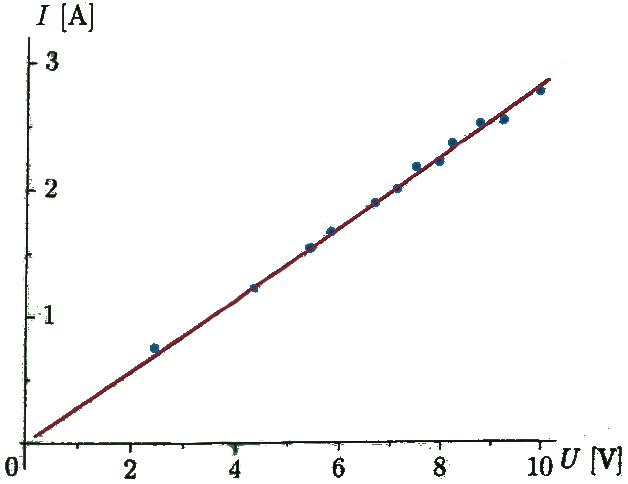
\includegraphics[width=0.8\linewidth]{mai_fig052.png}
  \captionof{figure}{Ověření Ohmová zákona lineární regresí.
  \cite[s.~263]{Musilova2009MA1}
  \label{mai:fig052}}
  \par}
  Pro odpor vychází \(R\doteq\SI{3.52}{\ohm}\). Součet čtverců odchylek přímky se směrnicí \(i/R
  = (1/\num{3.52})\Omega^{-1}\) od souboru bodů grafu je
  \begin{equation*}
    D(R) = \sum_{i=1}^{n}(U_i - R\cdot I_i)^2 \doteq\num{0.01},
  \end{equation*}
  \(\sigma(R) = \sqrt{D(R)/(n-1)}\doteq\sqrt{(\num{0.11}/11)}\doteq\num{0.03}\).  Graf přímky \(U
  = R\cdot I = \num{3.52}\cdot I\) proložené body je na obrázku \ref{mai:fig052}.
\end{mathexam}
      %---------------------------------------------------------------
      
      Popsaný způsob nalezení hodnoty elektrického odporu vodiče se nazývá\textbf{ metodou 
      nejmenších čtverců} (minimalizuje součet čtverců odchylek prokládané závislosti od souboru 
      naměřených bodů), v případě použití lineárního modelu, jako tomu bylo u Ohmová zákona, pak 
      jde o \textbf{lineární regresi}
      
      Obdobně se postupuje, je-li některá z měřených veličin lineární funkcí veličin jiných s 
      neznámými koeficienty lineární kombinace. Nechť
      \begin{equation*}
        Z = f(X_1, X_2, \ldots, X_K) = A_1X_1 + A_2X_2 + \cdots + A_KX_K.
      \end{equation*}
      Předpokládejme, že veličiny \(X_1, X_2, \ldots, X_K\) a \(Z\) měříme \(n\)-krát a naměříme 
      hodnoty
      \begin{equation*}
        X_j = \lbrace x_{j1}, \ldots x_{jn} \rbrace, \qquad 1 \leq j \leq K, \qquad 
        Z = \lbrace z_{1}, \ldots z_{n} \rbrace
      \end{equation*}
      Součet čtverců odchylek teoretické závislosti od naměřených bodů je
      \begin{equation*}
        D(Z) = \sum_{i=1}^{n}\left(z_i - \sum_{j=1}^{K}A_jx_{ji}\right)^2.
      \end{equation*}
      Nutnou podmínkou pro minimum tohoto výrazu jakožto funkce proměnných \(A_x, A_2, \ldots, A_K\)
      je platnost souboru rovnic
      \begin{equation*}
        \pder{D(Z)}{A_p} = 0 \Rightarrow 
        \sum_{i=1}^{n}2\left(z_i - \sum_{j=1}^{K}A_jx_{ji}\right)\cdot x_{pi} = 0
      \end{equation*}
      pro \(1 \leq i \leq n, 1 \leq j \leq K\). Tyto podmínky představují nehomogenní soustavu 
      \(K\) rovnic pro \(K\) neznámých \(( A_1, A_2, \ldots, A_K)\). Rozšířená matice soustavy je
      \begin{equation*}
        \overline{B} = (A|B) = 
          \left(
            \begin{array}{cccc|c}
              \sum_{i=1}^{n}x_{1i}x_{1i} & \sum_{i=1}^{n}x_{1i}x_{2i} & \cdots & 
              \sum_{i=1}^{n}x_{1i}x_{Ki} & \sum_{i=1}^{n}z_{i}x_{1i}                    \\
              \sum_{i=1}^{n}x_{1i}x_{1i} & \sum_{i=1}^{n}x_{2i}x_{2i} & \cdots & 
              \sum_{i=1}^{n}x_{2i}x_{Ki} & \sum_{i=1}^{n}z_{i}x_{2i}                    \\
                        \cdots           & \cdots & \cdots & \cdots   & \cdots          \\
              \sum_{i=1}^{n}x_{Ki}x_{1i} & \sum_{i=1}^{n}x_{Ki}x_{2i} & \cdots & 
              \sum_{i=1}^{n}x_{Ki}x_{Ki} & \sum_{i=1}^{n}z_{i}x_{Ki}                    \\
            \end{array}
          \right),
      \end{equation*}
      \begin{equation*}
        \sigma(z) = \sqrt{\dfrac{D(z)}{n - K}}.
      \end{equation*}
      V dalších kapitolách věnovaných lineární algebře se k tomuto problému znovu vrátíme a 
      ukážeme, že jej lze elegantně řešit také jako úlohu algebraickou, konkrétně úlohu o 
      ortogonální projekci vektorů na podprostory.
%} %tikzset
%---------------------------------------------------------------------------------------------------
\printbibliography[heading=subbibliography]
\addcontentsline{toc}{section}{Seznam literatury}